%Plantilla realizada por Felipe Garzon, basado en la platilla de WORD creada
%por el ing. Oscar Gelvez para el documento entregable en proyecto de grado II


\documentclass[12pt, letterpaper]{report}
% Definición de la línea gruesa idéntica a Thesis.cls


% --- PAQUETES ---
\usepackage[utf8]{inputenc}
\usepackage[spanish, es-tabla]{babel}
\usepackage{csquotes}
\usepackage[top=3cm, left=3cm, bottom=2cm, right=2cm]{geometry}

% ======== FUENTE: Times New Roman ========
\usepackage{mathptmx}
\usepackage[T1]{fontenc}
\usepackage[utf8]{inputenc}
\usepackage{tikz} 
 \usetikzlibrary{positioning, shapes.geometric, arrows.meta, shadows}
\usepackage{xcolor}
\usepackage{graphicx}
\graphicspath{{imagenes/}}
\usepackage{setspace}
\onehalfspacing 
\usepackage{titlesec}
\usepackage{tikz}
\usetikzlibrary{calc}
\usepackage{anyfontsize}
\usepackage{fancyhdr}
\usepackage{float}
\usepackage{listings}
\usepackage{caption}
\usepackage{booktabs}
\usepackage{tabularx}
\usepackage{caption}
\usepackage{multirow}
\usepackage{amsmath}
\usepackage{longtable}
\usepackage{float}
\usepackage{hyperref}
\hypersetup{
    colorlinks=true,
    linkcolor=black,
    citecolor=blue,    
    urlcolor=blue
}
\usepackage[backend=biber,style=ieee,sorting=none]{biblatex}
\addbibresource{Bibliography.bib}


% Colores USTA
\definecolor{ustaAzul}{RGB}{0,39,77}
\definecolor{ustaAmarillo}{RGB}{255,205,0}

% ============ INFORMACIÓN DEL PROYECTO (Editar aquí) ============
\newcommand{\proyectoTitulo}{DESARROLLO DE UNA APLICACIÓN WEB PARA LA GESTIÓN DE COMANDAS EN RESTAURANTES PYME CON ENCRIPTACIÓN Y AUTENTICACIÓN DE BAJO COSTO}%(RELACIÓN CON EL OBJETIVO GENERAL)
\newcommand{\estudianteUno}{LUIS FELIPE GARZÓN CAMACHO}
\newcommand{\estudianteDos}{NOMBRE DE ESTUDIANTE 2}
\newcommand{\proyectoModalidad}{Modalidad de Proyecto de Grado\\(Proyecto de Investigación)}
\newcommand{\grupoInvestigacion}{GRUPO DE INVESTIGACIÓN MEM} %MEM, GED
\newcommand{\lineaInvestigacion}{Modelado-Electrónica-Monitoreo}

% Directores y asesores
\newcommand{\director}{JAIME VITOLA OYAGA}
\newcommand{\directorTitulo}{Ph.D.} %(ACRÓNIMO CON MÁXIMO NIVEL DE FORMACIÓN)
\newcommand{\codirector}{JOHN MONZAIDE ALVAREZ CELY}
\newcommand{\codirectorTitulo}{MSc.} %(ACRÓNIMO CON MÁXIMO NIVEL DE FORMACIÓN)
\newcommand{\asesor}{JESÚS RENATO DE LA ROSA MARTÍNEZ}
\newcommand{\asesorTitulo}{Ing.} %(ACRÓNIMO CON MÁXIMO NIVEL DE FORMACIÓN)

% ======== FECHAS COMPLETAMENTE AUTOMÁTICAS ========
% Nombres de meses en español
\newcommand{\nombremes}[1]{%
  \ifcase#1\or enero\or febrero\or marzo\or abril\or mayo\or junio\or%
  julio\or agosto\or septiembre\or octubre\or noviembre\or diciembre\fi%
}

% Comandos de fecha automática (toma la fecha del sistema)
\newcommand{\proyectoAnio}{\the\year}
\newcommand{\proyectoMes}{\the\month}
\newcommand{\proyectoDia}{\the\day}
\newcommand{\proyectoMesTexto}{\nombremes{\month}}
\newcommand{\proyectoFecha}{\proyectoDia-\proyectoMes-\proyectoAnio}
\newcommand{\proyectoFechaCompleta}{\proyectoMesTexto{} de \proyectoAnio}

% ============ NOMBRES CORRECTOS ============
\addto\captionsspanish{
    \renewcommand{\contentsname}{CONTENIDO}
    \renewcommand{\listfigurename}{LISTA DE FIGURAS}
    \renewcommand{\listtablename}{LISTA DE TABLAS}
    \renewcommand{\lstlistlistingname}{LISTA DE CÓDIGOS}
}

% ============ CONFIGURACIÓN DE TÍTULOS ============
\newcommand{\bhrule}{{\color{black!50}\rule{\textwidth}{0.05pt}}}
% Formato de capítulos
\titleformat{\chapter}[hang]
  {\normalfont\Large\bfseries\centering}
  {\thechapter.}{10pt}{\MakeUppercase}
\titlespacing*{\chapter}{0pt}{-30pt}{20pt}

% Formato de secciones
\titleformat{\section}
  {\normalfont\large\bfseries}
  {\thesection.}{10pt}{}

\titleformat{\subsection}
  {\normalfont\normalsize\bfseries}
  {\thesubsection.}{10pt}{}

% ============ CONFIGURACIÓN DE CÓDIGO ============
\lstset{
    basicstyle=\ttfamily\small,
    breaklines=true,
    frame=single,
    numbers=left,
    numberstyle=\tiny,
    captionpos=b,
    showstringspaces=false
}

% Configuración de páginas
\pagestyle{fancy}
\fancyhf{}
\fancyhead[R]{\thepage}
\renewcommand{\headrulewidth}{0pt}

\begin{document}

% ==================== PRELIMINARES ====================
\pagenumbering{gobble}

%No editar amenos que el titulo no encaje bien

\begin{titlepage}
\begin{tikzpicture}[remember picture, overlay]
    % Fondo blanco 
    \fill[white] (current page.north west) rectangle ([xshift=9.5cm]current page.south west);
    
    % Franja amarilla vertical
    \fill[ustaAmarillo] ([xshift=13cm]current page.north west) rectangle ([xshift=13.28cm]current page.south west);
    
    % Fondo azul 
    \fill[ustaAzul] ([xshift=13.28cm]current page.north west) rectangle (current page.south east);
    
    % Año en la esquina superior derecha  
    \node[text=white, font=\fontsize{48}{58}\selectfont] at ([xshift=-4.56cm, yshift=-3cm]current page.north east) {\proyectoAnio};

    
    % --- BARRA NEGRA Y TÍTULO ---
    
    % 1. Barra negra más alta (de -7cm a -13cm para dar espacio)
    \fill[black] ([yshift=-7.5cm]current page.north west) rectangle ([xshift=19.5cm, yshift=-12.5cm]current page.north west);
    
    % 2. Título ajustado
    \node[
    text=white, 
    font=\fontsize{20}{24}\selectfont\bfseries, % Añadí negrita (\bfseries) para que se vea mejor
    anchor=center,       % Anclado al centro
    text width=18cm,     % ESTO ES CLAVE: Fuerza al texto a romperse en líneas
    align=center         % Centra el texto dentro del bloque
    ] at ([xshift=9.75cm, yshift=-10cm]current page.north west) % Coordenada: Mitad de ancho (19.5/2) y Mitad de altura (entre -7 y -13)
    {DESARROLLO DE UNA APLICACIÓN WEB PARA LA GESTIÓN DE COMANDAS EN RESTAURANTES PYME CON ENCRIPTACIÓN Y AUTENTICACIÓN DE BAJO COSTO};
    
    % Imagen  
     \node[anchor=west] at ([xshift=8.39cm, yshift=-4cm]current page.west) {
        % Ajusta el ancho (width) para que quepa en la zona blanca (< 8cm)
        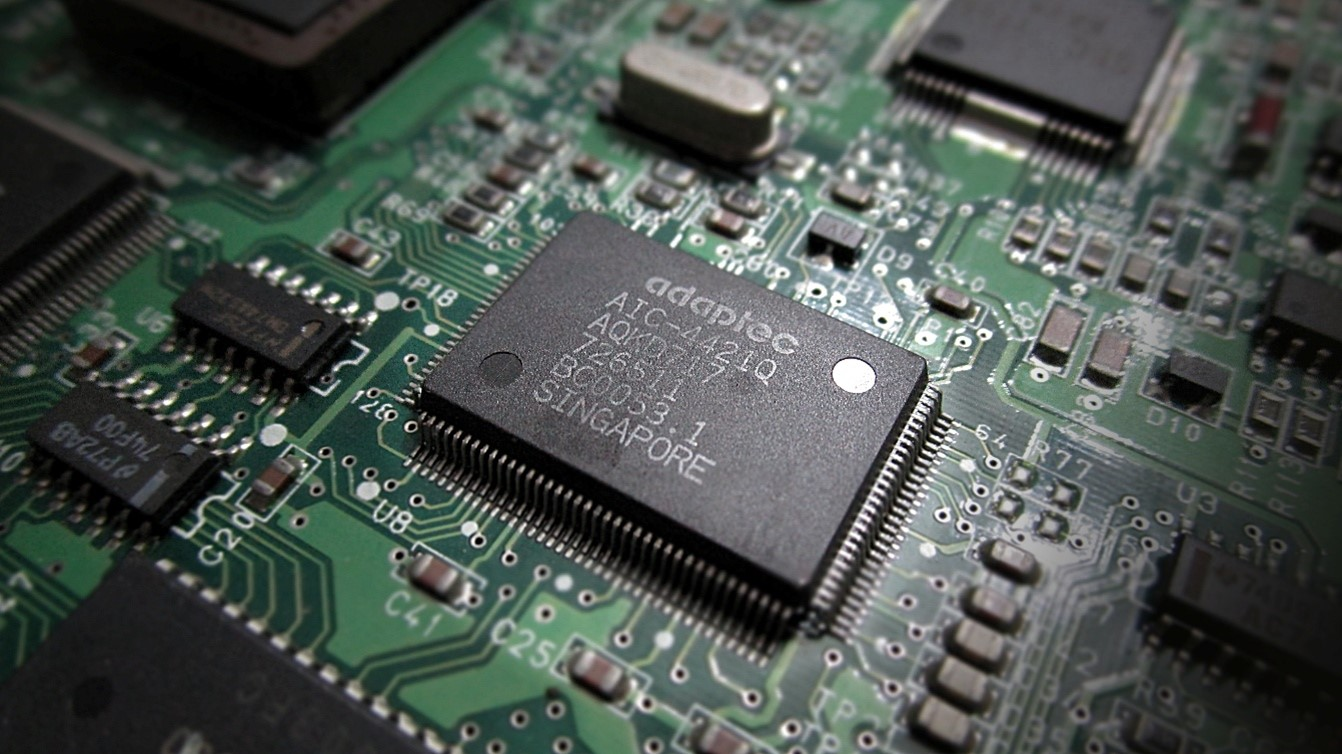
\includegraphics[width=13cm]{imagenes/pcb.jpg} 
    };
    
    % fecha
    \node[text=white, font=\fontsize{11}{13}\selectfont\normalfont, align=right, anchor=south east] 
        at ([xshift=-0.5cm, yshift=2.5cm]current page.south east) {
        \estudianteUno \\        
        Universidad Santo Tomás\\[0.3cm]
        \proyectoFechaCompleta
    };    
   
\end{tikzpicture}
\end{titlepage}

\newpage
\thispagestyle{empty}

\begin{center}   
    
    % Título 
    {\fontsize{11}{13}\selectfont\bfseries \proyectoTitulo\par} 
   
    
    \vspace{1.5cm}
    
    % Nombres estudiantes 
   {\fontsize{11}{13}\selectfont\bfseries \estudianteUno\par}
   %{\fontsize{11}{13}\selectfont\bfseries \estudianteDos\par}
    
    \vspace{1.5cm}
    
   % Modalidad - Arial 11.5
    {\fontsize{11.5}{14}\selectfont\bfseries \proyectoModalidad\par}
    
    % Logo USTA 
    \vspace*{1cm}
    
\includegraphics[width=0.6\textwidth]{logo_usta.png}
    
    \vspace{2.5cm}        
    
    % Grupo e investigación 
    {\fontsize{11.5}{14}\selectfont\bfseries \grupoInvestigacion\par}    
    {\fontsize{11.5}{14}\selectfont\bfseries \lineaInvestigacion\par}
    
    \vspace{1.5cm}    
    
    {\fontsize{11}{13}\selectfont\bfseries UNIVERSIDAD SANTO TOMÁS\par}
    {\fontsize{11}{13}\selectfont\bfseries FACULTAD DE INGENIERÍA ELECTRÓNICA\par}
    {\fontsize{11}{13}\selectfont\bfseries PROGRAMA DE INGENIERÍA ELECTRÓNICA\par}
    \vspace{1cm}
    {\fontsize{11}{13}\selectfont\bfseries Bogotá D.C.\par}
    {\fontsize{11}{13}\selectfont\bfseries \proyectoAnio\par}
     \vspace{1cm}
\end{center}
%%%%%%%%%%%%%%%%%%%%%%%%%%%%%%%%%%%%%%%%%%%%%%%%%%%%%%%%%
\newpage
\begin{center}    
    
   % Título 
    {\fontsize{11}{13}\selectfont\bfseries \proyectoTitulo\par}    
    \vspace{2cm}
    
   % Nombres estudiantes 
   {\fontsize{11}{13}\selectfont\bfseries \estudianteUno\par}
   \vspace{0.5cm}
   % {\fontsize{11}{13}\selectfont\bfseries \estudianteDos\par}
    
    \vspace{2cm}
    
    % Requisito - 
    {\fontsize{11.5}{14}\selectfont\bfseries Proyecto de grado presentado como requisito para optar al título de:\par}
    \vspace{0.3cm}
    {\fontsize{11.5}{14}\selectfont\bfseries Ingeniero Electrónico\par}
    
    \vspace{4.5cm}
    
    % Director 
    {\fontsize{11}{13}\selectfont\bfseries DIRECTOR DEL PROYECTO\par}
    \vspace{0.2cm}
    {\fontsize{11}{13}\selectfont \director{} (\directorTitulo)\par}
    
    \vspace{1.5cm}
    
    % Codirector 
    {\fontsize{11}{13}\selectfont\bfseries CODIRECTOR DEL PROYECTO\par}
    \vspace{0.2cm}
    {\fontsize{11}{13}\selectfont \codirector{} (\codirectorTitulo)\par}
    
    \vspace{1.5cm}
    
    % Asesor 
    %{\fontsize{11}{13}\selectfont\bfseries ASESOR DEL PROYECTO\par}
   %\vspace{0.2cm}
    %{\fontsize{11}{13}\selectfont \asesor{} (\asesorTitulo)\par}
    
    \vfill
    
    % Universidad 
    {\fontsize{11}{13}\selectfont\bfseries UNIVERSIDAD SANTO TOMÁS\par}
    {\fontsize{11}{13}\selectfont\bfseries FACULTAD DE INGENIERÍA ELECTRÓNICA\par}
    {\fontsize{11}{13}\selectfont\bfseries PROGRAMA DE INGENIERÍA ELECTRÓNICA\par}
    \vspace{0.2cm}
    {\fontsize{11}{13}\selectfont\bfseries Bogotá D.C.\par}
    {\fontsize{11}{13}\selectfont\bfseries \proyectoAnio\par}

    \vspace{1cm}  
\end{center}


%%%%%%%%%%%%%%%%%%%%%%%%%%%%%%%%%%%%%%%%%%%%%%%%%%%%%%%%%%%%%%%%%%%%%%%%%%%%
\newpage
\clearpage
\thispagestyle{empty}

\begin{center}
	{\bfseries\MakeUppercase{AUTORIDADES ACADÉMICAS}}
\end{center}

\vspace{1.5cm} 

\begin{flushright}
	\textbf{Fray Álvaro José Arango Restrepo, O.P.}\\
	Rector General
	
	\vspace{1cm}
	
	\textbf{Fray Hender Alveiro Rodríguez Pérez, O.P.}\\
	Vicerrector Administrativo y Financiero General
	
	\vspace{1cm}
	
	\textbf{Fray Adrián Mauricio García Peñaranda, O.P.}\\
	Vicerrector Académico General
	
	\vspace{1cm}
	
	\textbf{Dr. Anthony Numa Marín}\\
	Secretario General
	
	\vspace{1cm}
	
	\textbf{Fray Javier Antonio Hincapié Ardila, O.P.}\\
	Decano de División de Ingenierías
	
	\vspace{1cm}
	
	\textbf{Ing. Luz Patricia Rocha Caicedo}\\
	Secretaria de División de Ingenierías
	
	\vspace{1cm}
	
	\textbf{Ing. Leonardo Fabio Yepes Arbeláez}\\
	Decano Facultad de Ingeniería Electrónica
\end{flushright}

\vfill

\clearpage
\newpage
\thispagestyle{empty}
\begin{flushright}
    \noindent
    {\fontsize{14}{17}\selectfont \textbf{Nota de aceptación:}}
    
    \vspace{0.5cm}
    
    \noindent\makebox[0.7\textwidth]{\hrulefill}\\[0.2cm]
    \noindent\makebox[0.7\textwidth]{\hrulefill}\\[0.2cm]
    \noindent\makebox[0.7\textwidth]{\hrulefill}\\[0.2cm]
    \noindent\makebox[0.7\textwidth]{\hrulefill}\\[0.2cm]
    \noindent\makebox[0.7\textwidth]{\hrulefill}\\[0.2cm]
    \noindent\makebox[0.7\textwidth]{\hrulefill}\\[0.2cm]
    \noindent\makebox[0.7\textwidth]{\hrulefill}\\[0.2cm]
    \noindent\makebox[0.7\textwidth]{\hrulefill}\\[0.2cm]    
    
    \vspace{1.5cm}
    
    \noindent\makebox[0.7\textwidth]{\hrulefill}\\
    Firma del Director
    
    \vspace{1cm}
    
    \noindent\makebox[0.7\textwidth]{\hrulefill}\\
    Firma del Co-Director
    
    \vspace{1cm}
    
    \noindent\makebox[0.7\textwidth]{\hrulefill}\\
    Firma del Jurado 1
    
    \vspace{1cm}
    
    \noindent\makebox[0.7\textwidth]{\hrulefill}\\
    Firma del Jurado 2
    
    \vfill
\end{flushright}
\noindent
Bogotá D.C\\
Colombia\\
\proyectoFechaCompleta
 \vspace{1cm}

\newpage
\thispagestyle{empty}

\begin{center}
    {\fontsize{14}{17}\selectfont \textbf{ADVERTENCIA}}
\end{center}

\vspace{1cm}

\noindent
La Universidad Santo Tomás no se hace responsable de las opiniones y conceptos expresados en el trabajo de grado, solo velará por qué no se publique nada contrario al dogma ni a la moral católica y porque el trabajo no tenga ataques personales y únicamente se vea el anhelo de buscar la verdad científica.

\newpage
\begin{center}
	{\large\bfseries DEDICATORIA}
\end{center}

\vspace{2cm}

\begin{flushright}
	\textit{
		A mi madre, el pilar fundamental de mi existencia y el motor inagotable que me impulsa a despertar cada día con el firme deseo de alcanzar mis sueños. Cada paso que he dado en este largo camino universitario lleva impreso tu esfuerzo, tu amor infinito y tu fe inquebrantable en mí. Este logro es tan tuyo como mío, porque sin tus sabios consejos, tus sacrificios silenciosos y tu abrazo cálido en los momentos de mayor duda, nada de esto habría sido posible. Gracias por darme la vida y las alas para volar hasta aquí.
	}
	
	\vspace{1cm}
	
	\textit{
		A Angie Marcela Díaz, por ser mi luz, mi refugio y mi paz; eres como ese amanecer que llega otra vez para disipar mis dudas. Por brindarme tu amor y tu apoyo incondicional en absolutamente cada aspecto de mi vida. Gracias por tomar mi mano en los días de mayor estrés durante el desarrollo de este proyecto, por celebrar mis pequeñas victorias cotidianas, por escucharme con infinita paciencia y por creer en mí incluso cuando yo mismo dudaba. Tu presencia ha hecho que este arduo camino de la ingeniería sea mucho más hermoso y llevadero. Esta meta alcanzada también lleva tu nombre.
	}
	
	\vspace{1cm}
	
	\textit{
		A mi hermano Antonio Camacho y su esposo Edilberto Pérez, quienes fueron el impulso inicial que necesitaba para dar el primer y más importante paso hacia la universidad. Su confianza en mí llegó incluso antes que la mía propia, y sin ese apoyo generoso y decisivo, este sueño tal vez nunca habría encontrado su punto de partida. Gracias por animarme a creer que este camino también era posible para mí.
	}
\end{flushright}

\newpage
\thispagestyle{empty}

\begin{center}
	{\large\bfseries AGRADECIMIENTOS}
\end{center}

\vspace{1cm}

\noindent
El desarrollo de este proyecto no habría sido posible sin el apoyo incondicional de personas excepcionales que creyeron en este proceso.

Agradezco profundamente al ingeniero Jaime Vitola Oyaga, director de este proyecto, por su respaldo institucional, por confiar en esta propuesta tecnológica y por defender con firmeza este trabajo frente a la comunidad académica.

Al ingeniero John Monzaide Álvarez Cely, codirector de esta investigación, le expreso mi más sincera gratitud por su paciencia, su orientación detallada y por guiarme paso a paso en cada fase técnica y metodológica.

Un agradecimiento sumamente especial al ingeniero Jesús Renato De La Rosa Martínez, asesor del proyecto. Gracias por todo el conocimiento técnico compartido de manera desinteresada y por ser una guía invaluable a lo largo del desarrollo de este sistema. Por encima de todo, valoro enormemente su sincera amistad y su constante acompañamiento personal y profesional.

Al ingeniero Carlos Javier Mojica Casallas, docente de la facultad, quiero expresarle un profundo agradecimiento por su disposición constante, sus valiosos consejos y toda la ayuda brindada a lo largo de mi formación académica; sus enseñanzas fueron piezas clave en mi recorrido como estudiante.

Un reconocimiento muy especial y profundo a la docente Elizabeth Mayorga, quien con su dedicación me transmitió el verdadero amor por las matemáticas y fue la brújula principal que me encaminó hacia la ingeniería. Sin aquellas primeras experiencias de aprendizaje tan excepcionales e inspiradoras de su mano, recorrer este camino y alcanzar esta meta simplemente no habría sido posible. De igual forma, extiendo mi sincera gratitud a la profesora Dora Téllez por sus invaluables enseñanzas, y a los docentes Ericilia Pedraza y Eddy Alexander Galviz por su apoyo incondicional y calidad humana, tanto dentro como fuera de las aulas durante mi etapa escolar.


Finalmente, extiendo mi entera gratitud al señor Frank Muller y a todo el equipo de trabajo del restaurante Gastro Uno 58 Bar. Su gran generosidad al abrir las puertas de su establecimiento y permitir la activa participación de sus empleados durante la prueba piloto fue una pieza fundamental para materializar este proyecto y llevarlo a la realidad operativa. Gracias por su absoluta confianza.
\vspace{1cm}


\newpage
{\bfseries Conflicto de Intereses}


\vspace{1cm}

\noindent
Los autores declaran no tener ningún conflicto de intereses. Los patrocinadores no participaron en el diseño del estudio, la recopilación, el análisis ni la interpretación de los datos publicados, la redacción del documento.

\newpage
\chapter*{RESUMEN}
\addcontentsline{toc}{chapter}{Resumen}

La gestión manual de comandas en restaurantes de pequeña y mediana empresa (PYME) en 
Colombia genera pérdidas operativas, riesgos sanitarios y vulnerabilidades de seguridad 
informática que comprometen su viabilidad. Este trabajo presenta el diseño, implementación 
y evaluación de \textbf{QuickTable}, una aplicación web de bajo costo para la gestión 
integral de comandas en restaurantes PYME, que incorpora encriptación de base de datos y 
autenticación de doble factor (2FA) mediante hardware NFC local, operando íntegramente 
sobre una red de intranet sin dependencia de conectividad externa. El sistema fue 
desarrollado con .NET~8 (Razor Pages), Entity Framework~6, Microsoft SQL Server y 
AdminLTE como plantilla de interfaz, mientras que el módulo de seguridad física fue 
implementado sobre una Raspberry Pi~3 con lector RFID-RC522 a 13,56\,MHz (ISO/IEC~14443), 
controlado por un cliente Python con interfaz gráfica Tkinter. La validación se realizó 
mediante pruebas de concurrencia automatizadas, pruebas unitarias con MSTest, análisis de 
vulnerabilidades con OWASP ZAP 2.17.0, evaluación de rendimiento con Lighthouse y una 
implementación piloto en entorno real. Los resultados demuestran tasas de éxito 
transaccional superiores al 98\,\% bajo carga concurrente, tiempos de respuesta inferiores 
a 2 segundos, aprobación del conjunto completo de pruebas unitarias y un perfil de riesgo 
bajo según OWASP ZAP, confirmando la viabilidad técnica y económica de la solución como 
alternativa accesible a los sistemas POS comerciales disponibles en el mercado colombiano.

\bigskip
\noindent\textbf{Palabras clave:} gestión de comandas, aplicación web, PYME, encriptación, 
autenticación de doble factor, NFC, intranet, seguridad informática.


\chapter*{ABSTRACT}
\addcontentsline{toc}{chapter}{Abstract}

Manual order management in small and medium-sized restaurant enterprises (SMEs) in Colombia 
generates operational losses, sanitary risks, and information security vulnerabilities that 
threaten business viability. This paper presents the design, implementation, and evaluation 
of \textbf{QuickTable}, a low-cost web application for comprehensive order management in 
restaurant SMEs, incorporating database encryption and local NFC hardware-based two-factor 
authentication (2FA), operating entirely over an intranet without external internet 
dependency. The system was developed using .NET~8 (Razor Pages), Entity Framework~6, 
Microsoft SQL Server, and the AdminLTE interface template, while the physical security 
module was implemented on a Raspberry Pi~3 with an RFID-RC522 reader at 13.56\,MHz 
(ISO/IEC~14443), controlled by a Python client with a Tkinter graphical interface. 
Validation was conducted through automated concurrency testing, MSTest unit testing, 
OWASP ZAP 2.17.0 vulnerability analysis, Lighthouse performance evaluation, and a pilot 
deployment in a real operating environment. Results demonstrate transactional success rates 
above 98\,\% under concurrent load, response times below 2 seconds, full passage of the 
unit test suite, and a low-risk security profile per OWASP ZAP, confirming the technical 
and economic feasibility of the solution as an accessible alternative to commercial POS 
systems available in the Colombian market.

\bigskip
\noindent\textbf{Keywords:} order management, web application, SME, encryption, 
two-factor authentication, NFC, intranet, information security.




\newpage
\thispagestyle{empty}

\begin{center}
	{\large\bfseries GLOSARIO}
\end{center}

\vspace{1cm}

\noindent
\textbf{AES (\textit{Advanced Encryption Standard}):} Algoritmo de cifrado simétrico por bloques adoptado como estándar por el NIST, utilizado en este proyecto para cifrar los identificadores únicos (UID) de las tarjetas NFC asociadas a los administradores del sistema.

\noindent
\textbf{AJAX (\textit{Asynchronous JavaScript and XML}):} Técnica de desarrollo web que permite actualizar partes de una página de forma asíncrona sin necesidad de recargar el DOM completo, empleada en los módulos de Cocina y Caja para reflejar cambios de estado en tiempo real.

\noindent
\textbf{Autenticación:} Proceso de verificación de la identidad de un usuario, proceso o dispositivo, normalmente como requisito previo para conceder acceso a los recursos de un sistema.

\noindent
\textbf{Backend:} Capa de acceso a datos y lógica de negocio de una aplicación que no es visible para el usuario final, encargada del procesamiento y almacenamiento de la información.

\noindent
\textbf{BCrypt:} Función de hashing criptográfico adaptativa diseñada para el almacenamiento seguro de contraseñas. En este proyecto se aplica con factor de trabajo 12 para proteger las credenciales de acceso de los empleados almacenadas en la base de datos.

\noindent
\textbf{Bootstrap:} Framework CSS de código abierto que provee un sistema de grillas y componentes visuales responsivos. Se utiliza como base estructural del panel AdminLTE para garantizar la adaptabilidad de las vistas en dispositivos de distintas resoluciones.

\noindent
\textbf{Comanda:} Documento o registro donde se anotan las peticiones de los clientes en un establecimiento de hostelería para su transmisión a cocina y posterior facturación.

\noindent
\textbf{CRUD (\textit{Create, Read, Update, Delete}):} Conjunto de las cuatro operaciones básicas de persistencia de datos en una base de datos relacional: creación, lectura, actualización y eliminación de registros.

\noindent
\textbf{Encriptación:} Técnica de seguridad que consiste en transformar la información mediante algoritmos para asegurar su confidencialidad y evitar el acceso no autorizado.

\noindent
\textbf{Fómites:} Objetos o superficies inanimadas que pueden ser portadoras de agentes infecciosos y actuar como vehículos de transmisión de microorganismos.

\noindent
\textbf{Frontend:} Interfaz de usuario de una aplicación con la que el operador interactúa directamente para realizar tareas de gestión o visualización.

\noindent
\textbf{GPIO (\textit{General Purpose Input/Output}):} Conjunto de pines de propósito general presentes en plataformas de computación embebida como la Raspberry Pi, utilizados para establecer la comunicación física con periféricos externos mediante protocolos como SPI.

\noindent
\textbf{Hashing:} Proceso de transformar un dato de longitud arbitraria en una cadena de longitud fija mediante una función matemática unidireccional. A diferencia del cifrado, no es reversible, lo que lo hace idóneo para el almacenamiento seguro de contraseñas.

\noindent
\textbf{Inocuidad Alimentaria:} Garantía de que los alimentos no causarán daño al consumidor cuando se preparen o consuman de acuerdo con el uso al que se destinan.

\noindent
\textbf{Intranet:} Red de comunicaciones privada y confinada a la infraestructura física de una organización, que opera con los mismos protocolos que internet pero sin exposición a conectividad externa. En este proyecto, es el medio exclusivo de operación del sistema QuickTable.

\noindent
\textbf{LINQ (\textit{Language Integrated Query}):} Componente del ecosistema Microsoft .NET que permite expresar consultas sobre fuentes de datos (colecciones en memoria, bases de datos relacionales) usando sintaxis nativa de C\#, eliminando la escritura directa de sentencias SQL y mitigando por diseño vulnerabilidades de inyección.

\noindent
\textbf{ORM (\textit{Object-Relational Mapping}):} Técnica de programación que permite interactuar con una base de datos relacional mediante objetos del lenguaje de programación anfitrión, abstrayendo las operaciones de acceso a datos. En este proyecto se emplea Entity Framework 6 como ORM.

\noindent
\textbf{PYME:} Acrónimo de Pequeña y Mediana Empresa, empresas que cuentan con un número reducido de trabajadores y un volumen de facturación moderado.

\noindent
\textbf{Razor Pages:} Modelo de programación web incluido en el ecosistema .NET que estructura la aplicación orientada a páginas, acoplando la lógica del controlador y la vista en un mismo archivo \texttt{.cshtml} y su \textit{PageModel} asociado, simplificando el desarrollo frente al patrón MVC tradicional.

\noindent
\textbf{SPI (\textit{Serial Peripheral Interface}):} Protocolo de comunicación síncrona de bus serie utilizado para conectar la Raspberry Pi con el módulo lector RFID-RC522, mediante los pines físicos MOSI, MISO, SCK, SDA y RST.

\noindent
\textbf{UID (\textit{Unique Identifier}):} Identificador único grabado en fábrica en cada tarjeta o etiqueta NFC/RFID, empleado en este proyecto como credencial física de autenticación del administrador del sistema.

\noindent
\textbf{XSS (\textit{Cross-Site Scripting}):} Tipo de vulnerabilidad de seguridad web en la que un atacante inyecta código malicioso en páginas vistas por otros usuarios. Su mitigación se evalúa mediante el análisis de cabeceras de Política de Seguridad de Contenido (CSP) con OWASP ZAP.


\newpage
\thispagestyle{empty}

\begin{center}
	{\large\bfseries ABREVIATURAS}
\end{center}

\vspace{1cm}

\begin{description}
	\item[2FA] \textit{Two-Factor Authentication} (Autenticación de Dos Factores).
	\item[ACODRES] Asociación Colombiana de la Industria Gastronómica.
	\item[ACID] Atomicidad, Consistencia, Aislamiento y Durabilidad (propiedades transaccionales de bases de datos relacionales).
	\item[AES] \textit{Advanced Encryption Standard} (Estándar de Cifrado Avanzado).
	\item[AJAX] \textit{Asynchronous JavaScript and XML} (JavaScript y XML Asíncronos).
	\item[ANDI] Asociación Nacional de Empresarios de Colombia.
	\item[API] \textit{Application Programming Interface} (Interfaz de Programación de Aplicaciones).
	\item[BDD] \textit{Behavior-Driven Development} (Desarrollo Guiado por Comportamiento).
	\item[CSP] \textit{Content Security Policy} (Política de Seguridad de Contenido).
	\item[CRUD] \textit{Create, Read, Update, Delete} (Crear, Leer, Actualizar, Eliminar).
	\item[DANE] Departamento Administrativo Nacional de Estadística.
	\item[GPIO] \textit{General Purpose Input/Output} (Entrada/Salida de Propósito General).
	\item[JSON] \textit{JavaScript Object Notation} (Notación de Objetos JavaScript).
	\item[LINQ] \textit{Language Integrated Query} (Consulta Integrada al Lenguaje).
	\item[MVC] Modelo-Vista-Controlador (Patrón de arquitectura de software).
	\item[NFC] \textit{Near Field Communication} (Comunicación de Campo Cercano).
	\item[ORM] \textit{Object-Relational Mapping} (Mapeo Objeto-Relacional).
	\item[PIB] Producto Interno Bruto.
	\item[POS] \textit{Point of Sale} (Punto de Venta).
	\item[RFID] \textit{Radio Frequency Identification} (Identificación por Radiofrecuencia).
	\item[SPI] \textit{Serial Peripheral Interface} (Interfaz Periférica Serie).
	\item[TI] Tecnología de la Información (rol operativo del sistema con privilegios de gestión de seguridad).
	\item[TIC] Tecnologías de la Información y las Comunicaciones.
	\item[UID] \textit{Unique Identifier} (Identificador Único).
	\item[UML] \textit{Unified Modeling Language} (Lenguaje Unificado de Modelado).
	\item[XSS] \textit{Cross-Site Scripting} (Secuencias de Comandos entre Sitios).
	\item[ZAP] \textit{Zed Attack Proxy} (herramienta de análisis dinámico de seguridad de OWASP).
\end{description}
% ==================== ÍNDICES Y LISTAS ====================
\pagenumbering{roman}
\setcounter{page}{1}

% CONTENIDO
\tableofcontents
\newpage

\listoffigures
\addcontentsline{toc}{chapter}{Lista de Figuras}
\newpage


\listoftables
\addcontentsline{toc}{chapter}{Lista de Tablas}
\newpage



% ==================== LISTA DE CÓDIGOS (OPCIONAL) ====================
% Se agrega automáticamente. Cada código con caption=... aparecerá aquí.
% Para insertar código:
%   \begin{lstlisting}[language=Python, caption={Descripción}, label={lst:etiqueta}]
%   def funcion():
%       print("Hola")
%   \end{lstlisting}
% Descomenta si usas código en tu proyecto:
%
% \lstlistoflistings
% \addcontentsline{toc}{chapter}{Lista de Códigos}
% \newpage

% ==================== CONTENIDO PRINCIPAL ====================
\pagenumbering{arabic}
\setcounter{page}{1}

\chapter{INTRODUCCIÓN}

La industria gastronómica colombiana enfrenta una contradicción estructural: a pesar de 
constituir uno de los sectores productivos más dinámicos del país, con aproximadamente 
167.000 establecimientos registrados~\cite{acodres_estadisticas_2021} y un aporte del 
3,9\% al Producto Interno Bruto nacional equivalente a 56,7 billones de pesos en 
2022~\cite{andi_pib_2024}, la gran mayoría de sus operaciones cotidianas de gestión de 
pedidos se sostienen sobre un procedimiento manual: el mesero anota la orden del cliente 
en papel y la entrega físicamente a la cocina. Este método, históricamente aceptado por 
su bajo costo operativo inmediato, genera tres categorías de problemas que comprometen la 
viabilidad de los establecimientos de pequeña y mediana escala: ineficiencia operativa, 
riesgo sanitario e inseguridad de la información, todos susceptibles de ser mitigados 
mediante la adopción de tecnología digital adecuada a las condiciones reales del sector.

La dimensión operativa del problema está respaldada por evidencia cuantitativa concreta. 
Los sistemas basados en papel presentan tasas de error en pedidos de hasta el 8\%, frente al 2\% registrado en sistemas digitales, siendo la causa principal la mala 
interpretación de la caligrafía y el uso de abreviaturas en entornos de trabajo 
acelerado~\cite{Daniel2024, LSRetail2025}. La Asociación Nacional de Restaurantes de 
los Estados Unidos estima que este tipo de fallos puede traducirse en pérdidas equivalentes 
al 4\% de las ventas totales del establecimiento~\cite{Khan2023}, dado que 
aproximadamente el 60\% de los errores resultan en reemplazos gratuitos que el negocio 
debe asumir~\cite{Checkmate2025}. Esta presión económica adquiere una dimensión crítica 
en el contexto colombiano, donde la Asociación Colombiana de la Industria Gastronómica 
(ACODRES) estima que cuatro de cada diez restaurantes cierran durante sus primeros seis 
meses de operación~\cite{acodres_estadisticas_2021}. La imposibilidad de actualizar 
órdenes en tiempo real limita además la personalización del servicio y compromete la 
fidelización del cliente~\cite{Ser2024Estrategia}. A pesar de que las mejoras tecnológicas 
son conocidas, la implementación de sistemas digitales comerciales requiere una inversión 
inicial elevada en hardware, software y capacitación, sumada a costos de mantenimiento 
continuos que resultan poco accesibles para establecimientos con recursos 
limitados~\cite{marcelo2024desafios}.

La dimensión sanitaria, menos visible pero igualmente documentada, está asociada al papel 
como vehículo de transmisión de microorganismos. Stephens et al.~\cite{Stephens2019} 
demostraron en una revisión sistemática que los fómites constituyen un mecanismo de 
transmisión relevante para numerosos agentes infecciosos, y que las características físicas 
del soporte determinan directamente la tasa de supervivencia microbiana. Kirchner 
et al.~\cite{Kirchner2021} confirmaron que las superficies atípicas en entornos de 
servicio de alimentos, es decir, aquellas que quedan fuera de los protocolos de limpieza 
convencionales, actúan como vectores activos de contaminación cruzada. La comanda de papel 
recorre un circuito de múltiples manos (mesero, cocinero y cajero) sin protocolos de 
desinfección intermedios, y Hübner et al.~\cite{Huebner2011} demostraron experimentalmente 
que bacterias como \textit{Pseudomonas aeruginosa} y \textit{Enterococcus hirae} 
sobreviven en papel estándar durante al menos siete días y son recuperables mediante el 
ciclo de contacto mano--papel--mano. En el contexto colombiano, un análisis microbiológico 
en restaurantes formales e informales de Cali confirmó contaminación cruzada con altos 
porcentajes de bacterias mesófilas aerobias en superficies de contacto con 
alimentos~\cite{caro-hernandez_analisis_2020}, situación que contraviene directamente la 
Resolución 2674 de 2013 del Ministerio de Salud y Protección Social, que exige minimizar 
cualquier foco de contaminación que ponga en riesgo la inocuidad 
alimentaria~\cite{minsalud_resolucion2674_2013}.

La tercera dimensión del problema radica en la seguridad de la información. Las soluciones 
comerciales de gestión de comandas disponibles en el mercado colombiano (entre ellas 
GastroPOS~\cite{gastropos}, Loggro~\cite{loggro_planes}, Vendty~\cite{vendty} y 
Toteat~\cite{toteat_planes}) operan mayoritariamente bajo esquemas de suscripción mensual 
en la nube, sin contemplar de forma explícita mecanismos robustos de encriptación ni 
garantías sobre la custodia soberana de los datos del establecimiento. Esta estructura 
genera desconfianza en el operador, pues el control de información sensible (historiales 
de ventas, inventarios y preferencias de clientes) queda en manos de terceros. Para las 
PYME gastronómicas, que según la Encuesta de Micronegocios del DANE (EMICRON, primer 
trimestre de 2024) enfrentan limitaciones estructurales de inversión 
tecnológica~\cite{DANE2024}, esta barrera económica e informática consolida la resistencia 
a la digitalización y deja al sector en una situación de vulnerabilidad operativa y 
sanitaria sostenida.

Investigadores y desarrolladores de distintas latitudes han abordado problemas 
parcialmente similares al planteado en este trabajo. En el ámbito académico colombiano, 
Corredor Siratá~\cite{Documento2022} propuso un sistema POS web para la gestión de 
pedidos, evidenciando la necesidad de digitalización en el sector pero sin incorporar 
mecanismos de seguridad multicapa ni operación en entorno local. Desde España, Curieses 
Fernández~\cite{Curieses2023} y Bernat Elorza~\cite{Bernat2023} desarrollaron sistemas 
de gestión de comandas mediante aplicaciones web y dispositivos móviles, priorizando la 
usabilidad pero sin abordar la restricción de conectividad ni la protección de datos 
sensibles. En Latinoamérica, Escobar Vallejos~\cite{Escobar2023} y Allain 
Manrique~\cite{Allain2020} construyeron prototipos funcionales para establecimientos 
específicos, mientras que De Argila Lorente~\cite{deArgila2024} analizó la evolución 
de la gestión de comandas en tiempo real como parte de la transformación digital de la 
restauración española. En el plano técnico y operativo, Katagri y 
Balavalad~\cite{Katagri2025} documentaron reducciones del 40\% en tiempos de 
procesamiento de órdenes mediante automatización digital, y Sultana et 
al.~\cite{Sultana2024} propusieron un modelo basado en IoT para mejorar las operaciones 
de servicio de alimentos en países en desarrollo. Hummel y Murphy~\cite{EmilyHummel} 
demostraron mediante la técnica de planos de servicio que la estandarización de los 
canales de comunicación interna mejora directamente la eficiencia operativa, y De Vries 
et al.~\cite{DEVRIES201859} confirmaron que los sistemas digitales de pedido y pago 
impactan la retención de clientes y la frecuencia de visitas. Liyanage 
et al.~\cite{Liyanage2018} abrieron el precedente técnico de integración de tecnología 
NFC bajo el estándar ISO/IEC~14443 en sistemas de gestión de restaurantes. Sin embargo, 
ninguno de estos antecedentes aborda de forma integrada la restricción económica del 
hardware, la operación sin conectividad a internet, la encriptación de datos y la 
autenticación física como unidad funcional orientada específicamente al segmento PYME 
colombiano.

La pregunta que orienta esta investigación es: \textit{¿cómo desarrollar una aplicación 
	web de bajo costo para la gestión de comandas en restaurantes que garantice la seguridad 
	y confidencialidad de la información mediante encriptación y llaves físicas de acceso?} 
El objeto de estudio es el diseño, implementación y evaluación de \textbf{QuickTable}, 
un sistema web de gestión integral de comandas que digitaliza el ciclo operativo completo 
del restaurante (toma de pedidos, gestión en cocina y facturación en caja), incorporando 
encriptación de base de datos y autenticación de doble factor (2FA) basada en hardware 
NFC, operable sobre infraestructura de bajo costo en red de intranet local sin dependencia 
de conectividad externa. La hipótesis central del proyecto, planteada en el anteproyecto, 
sostiene que es posible construir una solución tecnológica accesible, segura y funcional 
para el sector gastronómico colombiano sin recurrir a servicios en la nube ni a hardware 
especializado de alto costo, siempre que se combinen adecuadamente tecnologías de software 
maduras con componentes electrónicos de bajo costo orientados a la seguridad por hardware.

El desarrollo de este proyecto se justifica por el impacto que genera en múltiples planos. 
En el plano operativo y económico, los restaurantes PYME que adopten la solución reducirán 
errores de pedido, acortarán tiempos de procesamiento de órdenes y obtendrán trazabilidad 
histórica de sus ventas con un costo de implementación sustancialmente inferior al de las 
alternativas comerciales existentes; los beneficiarios directos son los propietarios y 
administradores de establecimientos gastronómicos de pequeña y mediana escala, así como su 
personal operativo. En el plano sanitario, la eliminación del papel como medio de 
comunicación interna rompe activamente la cadena de transmisión de microorganismos entre 
áreas, constituyendo una medida preventiva que protege tanto al personal del 
establecimiento como a los clientes~\cite{minsalud_resolucion2674_2013}. En el plano 
informático, el modelo de despliegue local garantiza que el restaurante mantenga la 
custodia absoluta de su información financiera y operativa, y la encriptación de la base de 
datos junto con el módulo de autenticación física elevan el nivel de protección a un 
estándar que las soluciones comerciales del mercado colombiano no contemplan de forma 
integrada. Adicionalmente, el proyecto realiza un aporte metodológico al demostrar que los 
principios de la Ingeniería Electrónica (comunicaciones inalámbricas, sistemas embebidos y 
arquitecturas de seguridad) son aplicables a la solución de problemas reales del sector 
productivo nacional, diferenciando esta propuesta de los desarrollos puramente 
informáticos previos.

Para resolver el problema planteado se adoptó un enfoque de ingeniería orientado a la 
construcción e implementación real del sistema siguiendo una metodología en cascada. La 
aplicación web fue desarrollada sobre el framework .NET~8 con el modelo de páginas Razor 
Pages y Entity Framework~6~\cite{ef6_docs} como capa de acceso a datos sobre un motor 
Microsoft SQL Server, con una interfaz de usuario estructurada sobre la plantilla 
AdminLTE~\cite{BALSAM2025112186}. El módulo de seguridad por hardware se implementó 
mediante una Raspberry Pi~3 equipada con un lector RFID-RC522 operando a 13,56\,MHz 
conforme al estándar ISO/IEC~14443~\cite{Liyanage2018}, gestionada por un cliente Python 
con interfaz gráfica desarrollada en Tkinter. La validación del sistema se realizó mediante 
pruebas unitarias con MSTest, análisis de vulnerabilidades con OWASP~ZAP~2.17.0, pruebas 
automatizadas de concurrencia y una implementación piloto en entorno real sobre 
infraestructura deliberadamente limitada, con el fin de verificar la viabilidad del sistema 
en las condiciones reales del segmento objetivo.
\chapter{CONTEXTUALIZACIÓN}

\section{Planteamiento del problema}

En el contexto de la industria gastronómica colombiana, los sistemas de gestión de comandas\footnote{Según la RAE, «comanda» (del latín \textit{commanda}) se refiere a un \textit{«documento en que se encarga la ejecución de algo»}, específicamente en el contexto restaurantero sería \textit{«la nota donde se apuntan los pedidos de los clientes»} \cite{rae2024}.} siguen siendo predominantemente basados en procedimientos manuales, donde el personal de meseros transmite las órdenes de los clientes mediante notas escritas a mano que son físicamente entregadas al área de cocina. Aunque este método ha sido históricamente aceptado, su naturaleza primitiva genera desafíos operativos significativos. Entre los principales inconvenientes destacan los retrasos en la ejecución de platos debido a malentendidos en la lectura de las anotaciones, la pérdida accidental de comandas durante el traslado y errores en la facturación derivados de omisiones o doble registro de los ítems.

% --- Párrafo de contexto colombiano ---
Este escenario cobra especial relevancia al considerar la magnitud del sector en el país. En Colombia, existen aproximadamente 167,000 establecimientos gastronómicos registrados \cite{acodres_estadisticas_2021}, donde las Pequeñas y Medianas Empresas (PYME) constituyen la gran mayoría. Según cifras de la Asociación Nacional de Empresarios de Colombia (ANDI), el sector de alojamiento y servicios de comida representa el 3.9\% del Producto Interno Bruto (PIB) nacional, con un aporte de 56.7 billones de pesos en 2022 \cite{andi_pib_2024}. La Cámara del Sector Gastronómico de la ANDI, por sí sola, agrupa a más de 2,038 restaurantes que generan más de 34,822 empleos directos \cite{andi_gastronomia_2023}, lo que subraya la importancia de optimizar sus procesos operativos para garantizar su sostenibilidad y crecimiento.

Estas deficiencias operativas se traducen en cifras concretas. Estudios comparativos indican que los sistemas tradicionales basados en papel presentan una tasa de error en los pedidos de hasta un 8\%, en contraste con el 2\% de los sistemas digitales \cite{Daniel2024}. La causa principal de estas discrepancias se atribuye a errores humanos, como la mala interpretación de la caligrafía o el uso de abreviaturas, que son comunes en entornos de ritmo rápido \cite{LSRetail2025}. Según la Asociación Nacional de Restaurantes de Estados Unidos, este tipo de fallos puede generar pérdidas que ascienden a aproximadamente el 4\% de las ventas totales de un restaurante \cite{Khan2023}. El impacto económico es considerable, ya que se estima que el 60\% de los errores resultan en reemplazos gratuitos que el establecimiento debe asumir \cite{Checkmate2025}.

A pesar de las mejoras tecnológicas disponibles, el persistente uso de comandas físicas se atribuye en parte a la barrera económica que representan los sistemas digitales, cuya implementación requiere una inversión inicial elevada en hardware, software y capacitación, sumada a costos de mantenimiento continuos. Esta situación afecta particularmente a pequeños y medianos establecimientos, para los cuales la digitalización puede resultar poco accesible en comparación con métodos tradicionales de bajo costo operativo \cite{marcelo2024desafios}.

% --- Párrafo sobre vulnerabilidad de PYMES ---
Esta barrera es particularmente crítica en un sector con una alta tasa de mortalidad empresarial. Según la Asociación Colombiana de la Industria Gastronómica (ACODRES), se estima que cuatro de cada diez restaurantes en el país cierran durante sus primeros seis meses de operación, una estadística que resalta una vulnerabilidad estructural donde la ineficiencia operativa puede comprometer la viabilidad del negocio \cite{acodres_estadisticas_2021}. La presión por reducir costos fijos y variables lleva a que muchas PYME gastronómicas posterguen inversiones en tecnología, sin considerar que las pérdidas derivadas de errores manuales pueden superar con creces el costo de una digitalización planificada.

Estas deficiencias no solo impactan la eficiencia operativa de los procesos, sino que también inciden negativamente en la experiencia del cliente, al aumentar los tiempos de espera para la recepción de sus órdenes. La capacidad de realizar modificaciones o correcciones en los pedidos de forma rápida y precisa se ve restringida, lo que puede traducirse en pérdidas económicas tanto a corto como a largo plazo. Consecuentemente, esta problemática afecta la fidelización de los clientes y evidencia fallas en el sistema de gestión de comandas, comprometiendo la competitividad y sostenibilidad de los establecimientos. Asimismo, los incrementos en los tiempos de espera repercuten en la satisfacción del cliente y pueden derivar en notorias pérdidas financieras para el negocio.

Paralelamente a los desafíos operativos, el uso persistente de comandas físicas introduce un riesgo sanitario documentado que trasciende el ámbito de la eficiencia y compromete directamente la inocuidad alimentaria. Stephens et al. (2019) revisaron de manera sistemática la literatura científica sobre los fómites en el entorno construido, concluyendo que constituyen un mecanismo de transmisión relevante para numerosos microorganismos, en paralelo al contacto directo y a la transmisión aérea, y que las características del material del soporte físico inciden directamente sobre la supervivencia microbiana y la tasa de transferencia hacia y desde los humanos \cite{Stephens2019}. En el entorno de un restaurante, la comanda de papel recorre un circuito de múltiples manos: mesero, cajero y cocinero, sin que ninguno de estos puntos de transferencia contemple protocolos de desinfección intermedios, convirtiéndola en un eslabón activo dentro de la cadena de contaminación. Kirchner et al. (2021) demostraron precisamente que las superficies atípicas en entornos de servicio de alimentos, es decir, aquellas que habitualmente quedan fuera de los protocolos de limpieza convencionales, actúan como vectores activos de contaminación cruzada, y que la ausencia de rutinas de higiene específicas para este tipo de objetos perpetúa la transferencia de microorganismos entre el personal y las áreas de preparación de alimentos \cite{Kirchner2021}.

El riesgo particular que representa el papel como vehículo de transmisión ha sido comprobado experimentalmente. Hübner et al. (2011) inocularon papel de oficina estándar con cuatro cepas bacterianas de referencia \textit{Escherichia coli}, \textit{Staphylococcus aureus}, \textit{Pseudomonas aeruginosa} y \textit{Enterococcus hirae} y evaluaron su supervivencia durante siete días bajo condiciones ambientales normales. Los resultados demostraron que todos los microorganismos sobrevivieron en la superficie por un mínimo de 72 horas; de hecho, cepas como \textit{P. aeruginosa} y \textit{E. hirae} mantuvieron niveles de contaminación tan altos que, incluso al séptimo día de prueba, el material nunca alcanzó los umbrales mínimos para considerarse desinfectado. Para evaluar el riesgo de transmisión cruzada, la investigación reprodujo el ciclo de contacto mano--papel--mano, logrando recuperar bacterias viables en la segunda mano en la totalidad de los ensayos independientes, lo que confirma que el papel actúa como un intermediario altamente efectivo para la transferencia de patógenos. Además, los autores destacaron que la naturaleza porosa de este material presenta una resistencia inherente a los agentes químicos líquidos tradicionales. A diferencia de superficies no porosas como el acero inoxidable o el plástico, el papel se convierte en un reservorio persistente que no puede ser neutralizado mediante los métodos de higiene de uso habitual en cocinas \cite{Huebner2011}.

Esta vulnerabilidad adquiere una dimensión adicional cuando se considera la diversidad de agentes patógenos susceptibles de transmitirse a través de objetos de manipulación frecuente. Stephens et al. (2019) señalan que las nuevas herramientas de análisis molecular han evidenciado que los fómites también pueden vehiculizar comunidades microbianas completas y bacterias con resistencia a antibióticos, cuya transferencia indirecta en entornos no clínicos representa un riesgo emergente de especial relevancia en salud pública \cite{Stephens2019}. La relevancia de este riesgo se confirma en el contexto colombiano: un análisis microbiológico en restaurantes formales e informales y puestos de comida en Cali evidenció contaminación cruzada con altos porcentajes de bacterias mesófilas aerobias en superficies de contacto con alimentos, identificando géneros de la familia Enterobacteriaceae incluso en establecimientos de categoría formal \cite{caro-hernandez_analisis_2020}. Esta situación contraviene directamente la Resolución 2674 de 2013 del Ministerio de Salud y Protección Social, que exige a los establecimientos minimizar cualquier foco de contaminación que ponga en riesgo la inocuidad de los alimentos \cite{minsalud_resolucion2674_2013}.


%Paralelamente a estos desafíos operativos, emerge una preocupación crítica de carácter sanitario. El uso continuo de medios manuales, como lápiz y papel, para la comunicación entre áreas expone a riesgos de contaminación cruzada. En entornos donde el manejo frecuente de papeles por múltiples actores ocurre sin garantías de higienización intermedia, se facilita la transmisión de agentes patógenos \cite{Kirchner2021}. Esta situación, que ha cobrado especial relevancia en el contexto postpandemia, obliga tanto a consumidores como a reguladores a revaluar los estándares de seguridad e higiene en la cadena alimentaria. La carencia de un sistema digitalizado no solo limita la optimización de procesos, sino que también constituye una vulnerabilidad en términos de salud pública, comprometiendo la reputación del establecimiento y su cumplimiento con las normativas vigentes.


%La relevancia de este riesgo se confirma con estudios realizados en el contexto colombiano. Un análisis microbiológico en restaurantes formales e informales y puestos de comida en Cali, Colombia, evidenció "contaminación cruzada, con altos porcentajes en bacterias mesófilas aerobias" en superficies de contacto con alimentos \cite{caro-hernandez_analisis_2020}. Aunque la mayoría de los recuentos de coliformes totales se encontraron dentro del límite permisible, la identificación bacteriana demostró la presencia de varios géneros de la familia Enterobacteriaceae. Esta situación contraviene directamente las directrices establecidas en la Resolución 2674 de 2013 del Ministerio de Salud y Protección Social, que regula las buenas prácticas de manufactura y exige a los establecimientos minimizar cualquier foco de contaminación que ponga en riesgo la inocuidad de los alimentos \cite{minsalud_resolucion2674_2013}.


Adicionalmente a los desafíos operativos y sanitarios, el uso de sistemas manuales restringe la capacidad para gestionar cambios dinámicos en los pedidos y llevar un registro estructurado de la información generada. La imposibilidad de actualizar órdenes en tiempo real (sea para ajustar cantidades, modificar ítems del menú, incorporar preparaciones específicas o considerar alergias) propicia errores y confusiones que prolongan los tiempos de atención, repercutiendo negativamente en la satisfacción del cliente \cite{Ser2024Estrategia}. Igualmente, la falta de un registro sistematizado de los alimentos consumidos impide un análisis adecuado de tendencias de demanda, lo cual afecta la optimización de inventarios y la reducción de desperdicios, elementos esenciales para la sostenibilidad económica y ambiental de los establecimientos.

Por otro lado, es preciso destacar que uno de los limitantes más significativos que enfrentan algunos restaurantes al considerar la implementación de software de control de comandas radica en la incertidumbre respecto a la privacidad y seguridad de sus datos. Las soluciones comerciales predominantes dependen, en gran medida, del alojamiento de sus servidores en infraestructuras gestionadas por la misma empresa proveedora del servicio. Este modelo de servicio no contempla, de forma explícita, medidas robustas de encriptación ni garantías sobre el manejo seguro de la información sensible del restaurante. La carencia de certificaciones o protocolos de seguridad específicos genera desconfianza en el operador, ya que el control y la protección de datos vitales como historiales de ventas, inventarios y preferencias de los clientes, queda en manos de terceros. Esta situación representa no solo un riesgo de vulneración de información, sino que además limita la adopción de tecnologías digitales por parte de pequeños y medianos establecimientos, que perciben en este aspecto una barrera adicional frente a la modernización de sus procesos.

En el contexto de la digitalización, esta pregunta problemática invita a analizar de manera precisa cómo el uso de sistemas manuales puede limitar la eficiencia de los procesos operativos, comprometer la seguridad sanitaria y exponer la información sensible en restaurantes de pequeña y mediana escala. Se busca establecer una relación directa entre las deficiencias inherentes a los métodos tradicionales y los inconvenientes que estos generan, para así orientar el desarrollo de una solución tecnológica accesible y efectiva.



\section{Pregunta problema}

¿Cómo desarrollar una aplicación web de bajo costo para la gestión de comandas en restaurantes que garantice la seguridad y confidencialidad de la información mediante encriptación y llaves físicas de acceso?

\section{Objetivos}

\subsection{Objetivo General}
Desarrollar una aplicación web de creación y gestión de comandas para restaurantes que garantice la seguridad y confidencialidad de la información mediante mecanismos de encriptación y el uso de llaves físicas para el acceso administrativo, manteniendo un bajo costo de implementación y alta disponibilidad.

\subsection{Objetivos Específicos}
\begin{itemize}
	\item Diseñar la arquitectura general del sistema, estableciendo los requerimientos funcionales y no funcionales, así como los lineamientos de seguridad y escalabilidad.
	
	\item Implementar la solución tecnológica mediante la codificación y configuración de sus módulos principales, integrando el sistema de autenticación de doble factor basado en NFC con \textit{Raspberry Pi} y módulo \textit{RFID-RC522}.
	
	\item Evaluar el desempeño funcional y la seguridad del sistema mediante pruebas de laboratorio que midan tiempos de respuesta, tasas de éxito en operaciones de comandas, tiempo de autenticación NFC, y efectividad de los mecanismos de encriptación y control de acceso, verificando el cumplimiento de los requerimientos establecidos.
	
	\item Generar la documentación técnica y de usuario del sistema, comprendiendo manual técnico de instalación y configuración, y manual de usuario por roles, facilitando la transferencia de conocimiento y sostenibilidad del proyecto.
\end{itemize}



\section{Justificación}

La persistencia de métodos manuales en la gestión de comandas representa una oportunidad técnica para optimizar la comunicación interna y la experiencia del cliente mediante digitalización. Este proyecto desarrolla una solución web de bajo costo que transforma el proceso de gestión de pedidos en restaurantes PYME, haciéndolo accesible para establecimientos que enfrentan limitaciones económicas. Al eliminar la barrera de inversión inicial elevada característica de sistemas comerciales, la propuesta ofrece escalabilidad y rentabilidad sin comprometer funcionalidad, convirtiéndose en una alternativa viable para negocios de distintos tamaños que buscan modernizar sus operaciones con mínimo impacto financiero.

El contexto colombiano presenta una oportunidad significativa para esta solución. Según el DANE, la Encuesta de Micronegocios (EMICRON) del primer trimestre de 2024 evidencia la persistencia de micronegocios como motor económico del país \cite{DANE2024}, sector que enfrenta limitaciones estructurales de inversión tecnológica. Los beneficios técnicos y operativos del sistema se estructuran en seis ejes fundamentales:

\begin{itemize}
	\item \textbf{Estandarización del Flujo de Información:}   
	El sistema establece un canal digital unificado que conecta sala, cocina y caja mediante registros estructurados, eliminando la variabilidad inherente a las notas manuscritas. Investigaciones recientes demuestran que los sistemas tradicionales de pedidos son labor-intensivos, resultando en altas tasas de inexactitud en órdenes \cite{Sultana2024}, mientras que sistemas automatizados minimizan estos errores al asegurar colocación precisa y exacta de pedidos \cite{Sultana2024}. Al agilizar la comunicación entre clientes y personal de cocina, el sistema reduce errores, minimiza tiempos de procesamiento de órdenes y mejora la eficiencia del flujo de trabajo \cite{Katagri2025}.
	
	En el estudio de caso \textit{Using Service Blueprinting to Analyze Restaurant Service Efficiency} de Emily Hummel y Kevin S. Murphy\cite{EmilyHummel}, se demuestra que la eficiencia operativa mejora cuando la información se comunica de manera efectiva y estandarizada. El sistema propuesto logra precisamente esto al reemplazar la comunicación verbal y escrita, que es propensa a errores, por un registro digital único y consistente.
	
	
	\item \textbf{Trazabilidad Operativa en Tiempo Real:} 
	Más allá de la simple transmisión de pedidos, el sistema implementa capacidades de monitoreo temporal que registran cada modificación con marca de tiempo, identifica al responsable de cada operación y calcula métricas de servicio desde la toma del pedido hasta su entrega. Estudios académicos confirman que la automatización de la gestión de pedidos reduce el tiempo de procesamiento en aproximadamente 40\%, mientras que la eliminación de inexactitudes debidas a errores manuales mejora significativamente la satisfacción del cliente basada en retroalimentación de usabilidad \cite{Katagri2025}.
	
	Según De Vries, Roy y De Koste en el artículo \textit{Worth the wait? How restaurant waiting time influences customer behavior and revenue} \cite{DEVRIES201859}, la capacidad de los sistemas digitales para agilizar procesos de pedido y pago impacta directamente en la retención de clientes, la frecuencia de visitas y la duración de estancias \cite{DEVRIES201859}. El control temporal preciso que ofrece esta solución convierte estos beneficios en métricas medibles y gestionables.
	
	\item \textbf{Mitigación de Riesgos Sanitarios:} 
	La eliminación del papel como medio de transmisión de información entre áreas reduce vectores potenciales de contaminación cruzada. Si bien la literatura sobre contaminación específica en comandas es limitada, estudios sobre menús físicos demuestran que superficies manipuladas repetidamente sin protocolos de higienización sistemática presentan cargas microbiológicas significativas. 
	
	Investigaciones han evidenciado que los menús en papel, al ser manipulados repetidamente por clientes y personal, presentan altos niveles de contaminación \cite{alsallaiy2015}, y que la evaluación visual resulta insuficiente para garantizar limpieza \cite{choi2025}. Dado que las comandas manuscritas atraviesan un flujo similar de manipulación múltiple, la digitalización representa una medida preventiva al eliminar completamente este contacto físico entre áreas operativas.
	
	\item \textbf{Arquitectura de Seguridad Multicapa:} 
	La protección de información del establecimiento se implementa mediante dos mecanismos complementarios: encriptación de base de datos y autenticación física para acceso administrativo. La encriptación resguarda datos sensibles frente a accesos no autorizados incluso en caso de compromiso del servidor, mientras que la llave física desarrollada específicamente para este proyecto establece una barrera de acceso tangible que complementa controles digitales. Esta combinación de seguridad lógica y física genera un nivel de protección integral adaptado a las crecientes amenazas en entornos digitales, factor determinante para la confianza y adopción tecnológica en contextos donde la información operativa y financiera requiere máxima confidencialidad.
	
	\item \textbf{Integración Interdisciplinaria Hardware-Software:} 
	El proyecto constituye una aplicación integral de Ingeniería Electrónica al desarrollar un sistema embebido de autenticación mediante tecnología NFC acoplado a la aplicación web. La implementación de esta llave física de autenticación requiere conocimientos específicos de sistemas embebidos, protocolos de comunicación inalámbrica de corto alcance a frecuencia de 13.56 MHz conforme al estándar ISO/IEC 14443 \cite{Liyanage2018}, y arquitecturas de seguridad multicapa que combinan componentes electrónicos con algoritmos criptográficos. 
	
	Esta convergencia entre hardware especializado y desarrollo de software representa el núcleo de la formación en Ingeniería Electrónica, donde la comprensión de principios electromagnéticos, comunicaciones digitales y sistemas de control se aplican para resolver problemas reales de automatización y seguridad. El diseño del dispositivo NFC como mecanismo de autenticación física complementa controles lógicos implementados en software, demostrando la transversalidad característica de proyectos electrónicos modernos que trascienden el desarrollo puramente informático al integrar sensores, actuadores y sistemas de comunicación de bajo nivel con capas de aplicación de alto nivel \cite{Liyanage2018}.
	
	\item \textbf{Inteligencia Operativa Basada en Datos:} 
	El sistema transforma registros transaccionales en capacidades analíticas mediante el seguimiento sistemático de ingresos, gastos y patrones de consumo. Esta funcionalidad permite identificar tendencias de demanda, optimizar niveles de inventario y sincronizar tiempos de abastecimiento con necesidades reales, reduciendo desperdicio de alimentos con impacto económico y ambiental directo. Adicionalmente, el registro automático de horarios de entrada y salida del personal facilita la gestión de asistencia con datos precisos y confiables.
	
	Basado en la conclusión de Nabeel Salih Ali, Hasanein D. Rjeib, et al., en \textit{Automated attendance management systems: systematic literature review}, los sistemas de gestión de asistencia \textit{"proporcionan datos precisos y confiables, mejoran la eficiencia, facilitan el cumplimiento normativo y ofrecen datos útiles para la toma de decisiones"} \cite{Automatedattendance}, complementando las capacidades de gestión de comandas con control integral de recursos humanos.
\end{itemize}

La arquitectura técnica del sistema prioriza la optimización de recursos, permitiendo su operación en equipos con especificaciones computacionales básicas tanto para servidor como para base de datos. Esta característica elimina la necesidad de inversión en hardware especializado o servicios costosos de hosting en la nube, reduciendo significativamente barreras económicas para pequeños y medianos negocios. Al implementarse como aplicación web, el sistema garantiza compatibilidad universal con dispositivos heterogéneos \cite{BALSAM2025112186}, desde smartphones para toma de pedidos hasta computadoras para supervisión administrativa, independientemente del sistema operativo. La integración mediante red de intranet local elimina dependencias de conectividad externa a internet, suprimiendo gastos operativos recurrentes y reduciendo tanto el presupuesto de implementación inicial como los costos mensuales de operación \cite{akyildiz2006survey}.

En conjunto, estas características posicionan la solución como una herramienta de transformación integral para restaurantes que combina eficiencia operativa, adaptabilidad tecnológica y sostenibilidad económica. La convergencia de capacidades de gestión de pedidos, control de personal, análisis de datos operativos y seguridad multicapa diferencia esta propuesta de sistemas comerciales fragmentados que abordan aspectos aislados. Los indicadores cuantificables de impacto documentados en literatura académica incluyen reducción aproximada del 40\% en tiempo de procesamiento de órdenes y eliminación de inexactitudes por errores manauales \cite{Katagri2025}, métricas que justifican la inversión para el sector PYME colombiano. La incorporación de mecanismos de seguridad tanto sanitarios como informáticos provee garantías sobre confidencialidad y manejo seguro de información, factor decisivo para facilitar adopción tecnológica en un sector tradicionalmente resistente al cambio. El componente de ingeniería electrónica representado por el sistema embebido NFC conforme a estándares ISO/IEC 14443 \cite{Liyanage2018} demuestra la aplicación interdisciplinaria de conocimientos en comunicaciones inalámbricas, sistemas digitales y arquitecturas de seguridad, diferenciando este proyecto de desarrollos puramente informáticos. Estas ventajas consolidan la propuesta como una solución innovadora que impulsa la transformación digital en el sector gastronómico, contribuyendo al crecimiento económico y la sostenibilidad de establecimientos PYME.





\chapter{MARCO REFERENCIAL}

\section{Marco Conceptual}

Este capítulo establece los fundamentos técnicos y los estándares normativos que rigen la arquitectura y la ingeniería de la solución de software propuesta. A continuación, se detallan los principios de diseño, los modelos de estructuración de información y los marcos regulatorios internacionales que garantizan la viabilidad, escalabilidad y seguridad del sistema.

\subsection{Normativas IEEE Aplicables}
El desarrollo del sistema se rige por estándares internacionales de ingeniería de software para garantizar la calidad, mantenibilidad y escalabilidad del producto final:
\begin{itemize}
	\item \textbf{ISO/IEC/IEEE 29148 (Ingeniería de Sistemas y Software - Requisitos):} Establece los lineamientos rigurosos para la especificación de requerimientos de software (ERS), garantizando que las necesidades operativas se traduzcan en características técnicas medibles \cite{BALSAM2025112186}.
	\item \textbf{ISO/IEC/IEEE 23026:2023 (Ingeniería y Gestión de Sitios Web):} Define los requisitos de ingeniería, diseño, pruebas y mantenimiento para aplicaciones web en entornos de intranet, asegurando estándares de usabilidad, accesibilidad y seguridad de la información \cite{IEEE23026}.
	\item \textbf{IEEE 1016 (Estándar para el Diseño de Software):} Proporciona un marco metodológico para documentar la arquitectura del sistema, la estructuración de la base de datos relacional y las interfaces entre los componentes \cite{IEEE1016}.
\end{itemize}

\subsection{Aplicación Web y Arquitectura Intranet}
Una aplicación web es un sistema informático alojado en un servidor que procesa la lógica de negocio y entrega interfaces gráficas dinámicas al cliente a través de un navegador, independientemente de su sistema operativo. En este proyecto, la aplicación opera bajo una arquitectura de intranet local \cite{akyildiz2006survey}; esto significa que el servidor web y la red de acceso están confinados a la infraestructura física del restaurante, eliminando la dependencia a la conectividad externa a internet y reduciendo drásticamente la latencia de las peticiones.

\subsection{Patrón Arquitectónico Modelo-Vista-Controlador (MVC)}
El patrón MVC es un modelo de diseño de software que separa los datos de una aplicación, la interfaz de usuario y la lógica de control en tres componentes distintos. Esta separación de responsabilidades facilita el mantenimiento y el escalamiento del sistema:
\begin{itemize}
	\item \textbf{Modelo:} Representa la estructura de los datos y las reglas de negocio (entidades, validaciones y acceso a la persistencia).
	\item \textbf{Vista:} Corresponde a la interfaz gráfica generada dinámicamente que interactúa con el usuario final (mesero, cocinero o cajero).
	\item \textbf{Controlador:} Componente lógico que recibe las peticiones del cliente (HTTP), interactúa con el Modelo para obtener o mutar datos, y selecciona la Vista adecuada para retornar la respuesta.
\end{itemize}

\subsection{Almacenamiento de Datos}
El almacenamiento de datos en la ingeniería del proyecto comprende la persistencia estructurada y segura de la información transaccional. Para garantizar la integridad referencial y el cumplimiento estricto de las propiedades ACID (Atomicidad, Consistencia, Aislamiento y Durabilidad), se emplean bases de datos relacionales. En este entorno, los datos de inventario, ventas y sesiones de usuarios se almacenan en tablas interconectadas mediante llaves foráneas, lo que soporta altos volúmenes de transacciones concurrentes sin corrupción de datos y permite la implementación de mecanismos de encriptación en reposo.

\subsection{Procesamiento de Datos}
El procesamiento de datos en el contexto de esta aplicación web abarca la captura, transformación, validación y distribución de la información en tiempo real. Este flujo de datos va desde la intercepción de una petición (ej. la confirmación de una orden), hasta la ejecución de la lógica del servidor que calcula los subtotales de la transacción y realiza un \textit{push} de notificación a la interfaz de cocina. El diseño de algoritmos de procesamiento eficientes es vital para minimizar cuellos de botella en horas pico de operación.

\subsection{Ventajas de la Automatización de Procesos}
La automatización de procesos mediante sistemas de información centralizados elimina la intervención manual repetitiva. A nivel ingenieril y operativo, sus ventajas directas incluyen:
\begin{itemize}
	\item \textbf{Trazabilidad Continua:} Generación de un registro inmutable (logs) de cada acción ejecutada en el sistema, permitiendo auditar qué usuario creó, modificó o facturó una orden.
	\item \textbf{Reducción de Latencia Transaccional:} Comunicación instantánea y en tiempo real entre los nodos de la red local, eliminando los tiempos muertos de desplazamiento físico \cite{DEVRIES201859}.
	\item \textbf{Consistencia de la Información:} Mitigación de errores inducidos por fallos de memoria humana, caligrafía ilegible o errores de cálculo aritmético en la caja.
	\item \textbf{Inteligencia de Negocio:} Capacidad de procesar los grandes volúmenes de datos almacenados para extraer métricas precisas (platos más vendidos, horas pico, tiempos de preparación) de manera automática.
\end{itemize}

%%%%%%%%%%%%%%%%%%%%%%%%%%%%%%%%%%%%%%%%%%%%%%%%

\section{Marco Teórico}

\subsection{Fundamentos}
El proceso de transformación digital en las empresas del sector gastronómico representa un desafío sistémico que trasciende la simple adopción de equipos informáticos; exige una reingeniería profunda de los flujos de comunicación y la operatividad del negocio. Históricamente, la modernización de estos establecimientos ha enfrentado fuertes barreras de entrada debido a los altos costos de infraestructura, el pago de licencias corporativas y los contratos de mantenimiento forzosos \cite{marcelo2024desafios}. Los fundamentos teóricos de esta investigación se centran en el diseño de un paradigma de despliegue local (\textit{On-Premise}) de arquitectura ligera, en contraposición directa a los modelos de software como servicio (\textit{SaaS}) alojados en la nube. Este enfoque sustenta la viabilidad de un ecosistema digital robusto que otorga a los establecimientos plena propiedad sobre sus datos y garantiza una operación ininterrumpida, libre de la dependencia a redes de telecomunicaciones externas.


\subsection{Antecedentes Comerciales en Colombia y Análisis de Costos}

Para dimensionar la pertinencia de la solución propuesta, es indispensable
analizar el estado actual del mercado de software de Punto de Venta (POS)
orientado a restaurantes en Colombia. El ecosistema comercial está compuesto
principalmente por plataformas bajo esquemas de suscripción mensual o anual,
con estructuras de precios escalonadas según número de cajas, usuarios y
mesas habilitadas. La Tabla~\ref{tab:pos_colombia} presenta un resumen de
los planes base verificados a marzo de 2026.

\begin{itemize}
	
\item \textbf{GastroPOS (desde \$29.900 COP/mes):}
Desarrollada por la empresa colombiana del mismo nombre, GastroPOS
estructura su oferta en dos categorías de planes \cite{gastropos}:

\begin{itemize}
	\item \textbf{Planes sin Facturación Electrónica:}
	\begin{itemize}
		\item \textbf{Restobar POS (\$29.900 COP/mes):} Plan de entrada
		orientado a restaurantes y bares, sin módulo de facturación
		electrónica DIAN.
		\item \textbf{Tienda POS (\$39.900 COP/mes):} Variante orientada
		a comercios de venta al detal, igualmente sin facturación
		electrónica incluida.
	\end{itemize}
	\item \textbf{Planes con Facturación Electrónica DIAN:}
	\begin{itemize}
		\item \textbf{Plan Básico (\$41.900 COP/mes):} Hasta 200 facturas
		electrónicas mensuales.
		\item \textbf{Plan Plus (\$84.900 COP/mes):} Hasta 500 facturas
		electrónicas mensuales.
		\item \textbf{Plan Premium (\$149.900 COP/mes):} Hasta 1.000
		facturas electrónicas mensuales.
	\end{itemize}
\end{itemize}

Los planes con facturación electrónica establecen un límite mensual de
documentos; cuando el volumen del establecimiento supera el techo del
plan contratado, se requiere migrar al nivel inmediatamente superior
\cite{gastropos}.
	
	\item \textbf{Loggro Restobar (\$120.990 / \$175.990 / \$219.990
		COP/mes):}
	Plataforma en la nube con tres niveles de plan comercializados
	directamente en su sitio:
	
	\begin{itemize}
		\item \textbf{Plan Básico (\$120.990/mes):} Habilita 1 caja,
		3 usuarios, 15 mesas y 30 facturas electrónicas incluidas. Incluye
		POS online ilimitado, inventario con recetas ilimitado, 1 zona de
		comandas, toma de pedidos desde el móvil, menú digital con código
		QR y gestión de gastos.
		\item \textbf{Plan Estándar (\$175.990/mes):} Amplía la operación
		a 2 cajas, 6 usuarios, 30 mesas y 3 zonas de comandas, manteniendo
		las demás características del plan base.
		\item \textbf{Plan Premium (\$219.990/mes):} Soporta hasta 5
		cajas, usuarios ilimitados, 200 mesas y zonas de comandas
		ilimitadas.
	\end{itemize}
	
	Los tres planes incluyen las primeras 30 facturas electrónicas
	mensuales; a partir de ese volumen, la facturación electrónica
	ilimitada se contrata como complemento desde \$45.990 COP/mes según
	el nivel de facturación del establecimiento. Otros
	complementos disponibles son: caja adicional (\$43.990/mes), zona de
	comanda adicional (\$18.990/mes), usuario adicional (\$18.990/mes),
	mesa adicional (\$8.990/mes) y nómina electrónica (desde
	\$18.990/mes) \cite{loggro_planes}.
	
	\item \textbf{Vendty (desde \$100.000 COP/mes en pago mensual):}
	Con más de diez años en el mercado colombiano, Vendty estructura su
	oferta en tres planes:
	
	\begin{itemize}
		\item \textbf{Plan Emprendedor (\$100.000/mes o \$1.000.000/año):}
		2 usuarios, 1 caja, 20 mesas, productos ilimitados, facturas POS
		ilimitadas y hasta 1.000 facturas electrónicas mensuales.
		\item \textbf{Plan Profesional (\$150.000/mes o \$1.500.000/año):}
		5 usuarios, 2 cajas, 35 mesas y tienda virtual integrada.
		\item \textbf{Plan Empresarial (\$200.000/mes o \$2.000.000/año):}
		10 usuarios, 5 cajas, 50 mesas, tienda virtual avanzada, acceso
		a API e integración con versión de escritorio.
	\end{itemize}
	
	Todos los planes incluyen capacitación, actualizaciones y soporte, y
	son compatibles con hardware genérico: tablet Android, PC, Mac,
	impresoras de tiquete, lectores de código de barras y cajones de dinero. Vendty también comercializa una versión de escritorio con
	estructura de precios diferente: el plan anual desde \$85.000 COP/mes
	(pago único anual de \$1.020.000), orientada a operaciones sin
	dependencia de navegador \cite{vendty_escritorio}. El sitio oficial
	indica adicionalmente que para establecimientos tipo restaurante puede
	aplicar un valor diferenciado al de comercios retail \cite{vendty}.
	
	\item \textbf{Toteat (desde \$139.900 COP/mes + 0,7\% sobre venta neta):}
	Plataforma de origen chileno con operación activa en Colombia, Toteat
	aplica un modelo de precios compuesto por una tarifa base mensual más
	un porcentaje variable calculado sobre la venta neta mensual del
	establecimiento, más impuestos. Sus planes son:
	
	\begin{itemize}
		\item \textbf{Plan Básico (\$139.900 COP/mes + 0,7\% sobre venta
			neta):} Incluye POS en la nube, usuarios y mesas ilimitados,
		impresión de comandas, integración con hasta 3 aplicaciones de
		\textit{delivery}, boleta y factura electrónica ilimitada, menú QR
		digital, modo \textit{offline}, integración con medios de pago
		digitales y reportes estratégicos \cite{toteat_planes}.
		\item \textbf{Plan Corporativo (\$459.900 COP/mes + 0,35\% sobre
			venta neta):} Reduce el porcentaje variable a la mitad e incorpora
		funcionalidades para operaciones multi-sede, acceso a APIs de
		inventario, compras y ventas, módulo de reservas y un gestor de
		cuenta dedicado \cite{toteat_corp}.
	\end{itemize}
	
	La plataforma registra una calificación de 4,5/5 en Capterra Colombia
	al cierre de 2025, con soporte personalizado 24/7 incluido en todos sus
	planes \cite{capterra_toteat}.
	
	\item \textbf{Poster POS (precio en USD, variable según tasa de
		cambio):}
	Plataforma de origen ucraniano disponible en Colombia, Poster estructura
	sus planes en tres niveles (Mini, Business y Pro), diferenciados por la
	cantidad máxima de platillos y artículos registrables: 100, 300 y 1.500
	respectivamente para el módulo restaurante.
	Los precios se publican en dólares estadounidenses en su sitio oficial,
	por lo que el costo mensual en pesos colombianos está sujeto a la
	variación de la tasa de cambio \cite{comparasoftware_poster}. La
	integración con la DIAN para facturación electrónica en Colombia se
	gestiona mediante una aplicación complementaria de terceros
	denominada ``Facturación Electrónica Colombia'', disponible en el
	directorio de integraciones de Poster \cite{poster_dian}.
	
\end{itemize}

\begin{table}[h!]
	\centering
	\caption{Comparativa técnica y comercial de software POS para restaurantes en Colombia (Marzo 2026)}
	\label{tab:pos_colombia}
	\small
	% Definimos columnas: l (Software), X (Plan), r (Costo), c (Cajas), c (Usuarios), l (FE DIAN)
	\begin{tabularx}{\textwidth}{l X r c c l}
		\toprule
		\textbf{Software} & \textbf{Plan} & \textbf{Costo (COP/mes)} & \textbf{Cajas} & \textbf{Usu.} & \textbf{FE DIAN} \\
		\midrule
		\multirow{2}{*}{GastroPOS} 
		& Restobar & \$29.900 & NA & NA & Complemento \\
		& Básico con FE & \$41.900 & NA & NA & Incluida (200) \\
		\midrule
		\multirow{3}{*}{Vendty} 
		& Emprendedor & \$100.000 & 1 & 2 & Incluida (1.000) \\
		& Profesional & \$150.000 & 2 & 5 & Incluida (1.000) \\
		& Empresarial & \$200.000 & 5 & 10 & Incluida (1.000) \\
		\midrule
		\multirow{3}{*}{Loggro} 
		& Básico & \$120.990 & 1 & 3 & Parcial (30) \\
		& Estándar & \$175.990 & 2 & 6 & Parcial (30) \\
		& Premium & \$219.990 & 5 & Ilimit. & Parcial (30) \\
		\midrule
		\multirow{2}{*}{Toteat} 
		& Básico & \$139.900 + 0,7\%\textsuperscript{*} & NA & Ilimit. & Incluida \\
		& Corporativo & \$459.900 + 0,35\%\textsuperscript{*} & NA & Ilimit. & Incluida \\
		\midrule
		Poster & Mini / Biz / Pro & Variable (USD) & NA & NA & Terceros \\
		\bottomrule
	\end{tabularx}
	\begin{flushleft}
		\footnotesize
		\textbf{FE}: Facturación Electrónica (documentos/mes). \textbf{NA}: No especificado por el proveedor. \textbf{Ilimit.}: Ilimitados. \\
		\textsuperscript{*} Porcentaje calculado sobre la venta neta mensual. \\
		\textbf{Fuentes}: \cite{gastropos}, \cite{vendty}, \cite{loggro_planes}, \cite{toteat_planes}, \cite{comparasoftware_poster}.
	\end{flushleft}
\end{table}


\subsection{Tecnologías Implementadas y su Relación Costo-Beneficio}
El desarrollo técnico del sistema se estructuró a partir de una selección rigurosa de herramientas que garantizan un rendimiento de nivel empresarial y altos estándares de seguridad, minimizando a su vez los costos de licenciamiento de software.

\subsubsection{Framework .NET 8 (Razor Pages)}
El núcleo de la aplicación se fundamenta en .NET 8, un entorno de ejecución de alto rendimiento. La elección del modelo de desarrollo \textit{Razor Pages} permite procesar y acoplar la interfaz de usuario junto con la lógica de negocio directamente en el lado del servidor de forma cohesiva. Esta arquitectura acelera los tiempos de desarrollo y facilita el despliegue del software en equipos con recursos de hardware limitados, evitando la sobrecarga inherente a arquitecturas fragmentadas.

\subsubsection{Entity Framework 6 y SQL Server}
Para la persistencia de datos se emplea \textbf{Entity Framework 6} (EF6),
un Mapeador Objeto-Relacional (ORM) de Microsoft que abstrae las operaciones
de acceso a datos mediante un modelo de entidades en C\#, eliminando la
escritura directa de sentencias SQL para las operaciones estándar
\cite{ef6_docs}. Como motor de base de datos se utiliza \textbf{SQL Server},
disponible en las ediciones Express y Developer sin costo de licenciamiento
para desarrollo y despliegue en entornos de producción no comerciales de
pequeña escala \cite{sqlserver_editions}. La combinación de EF6 con SQL
Server es compatible de forma nativa con .NET 8 mediante el paquete
\texttt{EntityFramework} 6.5.x disponible en NuGet \cite{ef6_nuget}.

\subsubsection{Diseño Frontend y Estructuración de Interfaz}
La capa de presentación del sistema se implementó utilizando como base estructural el panel de control de código abierto \textit{AdminLTE}, el cual opera sobre el framework CSS Bootstrap. El uso de este recurso proporcionó un sistema de grillas predefinido y componentes visuales estándar (como tablas, formularios y modales) que aseguran la responsividad de la aplicación en diferentes tamaños de pantalla (computadoras, tabletas y teléfonos móviles). 

A partir de esta base técnica, el código del \textit{frontend} fue depurado y adaptado para construir interfaces segregadas según el sistema de control de acceso basado en roles. De este modo, se desarrollaron vistas independientes que exponen únicamente las funcionalidades permitidas para cada perfil de usuario: un módulo simplificado para la toma de comandas por parte de los meseros, un panel de gestión de colas de preparación para la cocina, y una interfaz administrativa orientada a la gestión de inventarios y facturación.

\subsubsection{Módulo de Seguridad Físico}
En soluciones comerciales de alta gama, la implementación de controles de acceso de doble factor o autenticación por hardware supone la adquisición de periféricos costosos. Para democratizar este nivel de protección, el proyecto integra una \textbf{Raspberry Pi} que actúa como unidad de procesamiento para un módulo lector \textbf{RFID-RC522}. Este conjunto gestiona la lectura de etiquetas físicas NFC, habilitando la creación de llaves de acceso encriptadas indispensables para ingresar a la administración del sistema.

%%%%%%%%%%%%%%%%%%%%%%%%%%%%%%%%%%%%%%%%%%%%%%%%%%%%%%%%

\section{Marco Legal}
El despliegue de soluciones tecnológicas en el sector comercial colombiano debe enmarcarse dentro de la legislación vigente respecto al tratamiento de la información, el uso de medios electrónicos y la infraestructura tecnológica. Al tratarse de un sistema \textit{On-Premise} (alojado localmente en las instalaciones del restaurante), aplican consideraciones jurídicas específicas.

\subsection{Regulación sobre Protección de Datos Personales}
En Colombia, la Ley 1581 de 2012 y sus decretos reglamentarios establecen el Régimen General de Protección de Datos Personales (Habeas Data) \cite{ley1581}. Esta normativa obliga a las entidades que recolectan, almacenan o procesan información personal a implementar políticas estrictas de privacidad y solicitar autorización expresa a los titulares. 

En el contexto de la presente investigación, la arquitectura del sistema ha sido diseñada bajo el principio de \textit{minimización de datos}. La aplicación gestiona exclusivamente información de carácter transaccional y operativo como lo son comandas, flujo de caja y roles de empleados internos; sin requerir, capturar ni almacenar datos personales sensibles de los clientes comensales (como nombres, documentos de identidad, teléfonos o correos electrónicos). En consecuencia, el sistema mitiga el riesgo jurídico asociado al manejo de datos de terceros y exime al establecimiento de obligaciones complejas frente a la Superintendencia de Industria y Comercio (SIC) en materia de bases de datos de clientes.

\subsection{Normativas TIC sobre Almacenamiento y Medios Electrónicos}
La legislación colombiana, a través de la Ley 527 de 1999, reconoce la validez jurídica y la fuerza probatoria de los mensajes de datos y registros electrónicos, equiparándolos a los documentos físicos \cite{ley527}. Esto otorga pleno respaldo legal a las comandas y auditorías generadas digitalmente por el sistema. 

Respecto al almacenamiento de la información, el sistema adopta un modelo local en lugar de la tercerización en la nube. Mantener la base de datos de forma local a través de SQL Server centraliza la custodia de los activos de información bajo el control absoluto del restaurante. Esto facilita la implementación de políticas de almacenamiento estructurado (información de acceso inmediato para la operación diaria, e información en copias de seguridad encriptadas) sin exponer los registros financieros a vulnerabilidades inherentes a servidores públicos de internet.

\subsection{Legislación sobre Delitos Informáticos}
La Ley 1273 de 2009 modificó el Código Penal colombiano para crear un nuevo
bien jurídico tutelado denominado ``de la protección de la información y de
los datos'', e introdujo tipos penales específicos para conductas que afecten
sistemas informáticos. Entre los artículos de mayor relevancia
para el presente proyecto se encuentran:

\begin{itemize}
	\item \textbf{Artículo 269A -- Acceso abusivo a un sistema informático:}
	Tipifica el acceso no autorizado, total o parcial, a un sistema
	informático protegido o no con medida de seguridad, con penas de 48 a
	96 meses de prisión y multas de 100 a 1.000 salarios mínimos legales
	mensuales vigentes.
	\item \textbf{Artículo 269C -- Interceptación de datos informáticos:}
	Penaliza la interceptación de datos en su origen, destino o en el
	interior de un sistema informático sin autorización judicial previa.
	\item \textbf{Artículo 269F -- Violación de datos personales:}
	Sanciona la obtención, compilación, sustracción, venta o envío de datos
	personales contenidos en ficheros, archivos o bases de datos sin
	consentimiento del titular.
\end{itemize}

El mecanismo de autenticación de doble factor implementado en el sistema,
basado en tarjetas NFC con identificadores encriptados, opera como una
medida de seguridad en los términos del Artículo 269A, dado que condiciona
el acceso administrativo a la posesión física de un elemento hardware y al
conocimiento de credenciales. Adicionalmente, el cifrado de la base de datos
restringe la legibilidad de los registros almacenados ante cualquier acceso
no autorizado al servidor, en concordancia con el espíritu protector del
Artículo 269F \cite{ley1273}.

%%%%%%%%%%%%%%%%%%%%%%%%%%%%%%%%%%%%%%%%%%%

\section{Marco Ambiental}
La transición de procesos análogos a digitales conlleva implicaciones directas sobre el medio ambiente. El análisis de estas implicaciones requiere evaluar tanto los beneficios derivados de la desmaterialización de los procesos, como el impacto energético de la infraestructura tecnológica requerida.

\subsection{Legislación y Estrategias de Cero Papel}
El Estado colombiano ha promovido activamente la reducción del consumo de recursos físicos en entornos administrativos y comerciales. Directrices como el Decreto Ley 2106 de 2019 impulsan la iniciativa \textit{Cero Papel}, orientada a sustituir flujos de trabajo físicos por medios electrónicos para lograr una gestión más eficiente y sostenible \cite{dec2106}. 

La digitalización del ciclo de comandas mediante el sistema propuesto elimina la dependencia del papel convencional utilizado en las comandas manuscritas de los restaurantes. Esta supresión de insumos de un solo uso no solo disminuye los costos operativos fijos del establecimiento, sino que reduce directamente la generación de residuos sólidos, alineando la operación del negocio con las políticas nacionales de sostenibilidad y economía circular \cite{UNSDS}.

\subsection{Impacto Energético de la Infraestructura de Servidores}
A nivel global, la proliferación de la computación en la nube ha generado preocupación medioambiental. Las granjas de servidores (\textit{Data Centers}) requeridas para soportar los modelos comerciales de \textit{Software as a Service (SaaS)} consumen cantidades masivas de energía eléctrica y agua dulce para el enfriamiento de sus procesadores. Regulaciones internacionales recientes exigen monitorear métricas críticas como la Eficiencia en el Uso de la Energía (PUE) y el Carbono (CUE), evidenciando el alto impacto ecológico del almacenamiento en la nube a gran escala.

En contraposición, la solución tecnológica abordada en este proyecto minimiza significativamente la huella de carbono asociada al hardware. El sistema evita la dependencia de macro-servidores externos, ejecutando toda la lógica de negocio y base de datos sobre la infraestructura computacional de bajo consumo existente en el local (computadores convencionales) y microcontroladores de arquitectura ARM (como la \textit{Raspberry Pi} empleada para el módulo de seguridad). Estos dispositivos operan con voltajes reducidos, lo que garantiza un consumo eléctrico mínimo y nulo requerimiento de refrigeración industrial, demostrando que la automatización de procesos locales puede lograrse con un impacto ambiental marginal en términos de consumo energético.

\chapter{DESARROLLO}

Este capítulo detalla el proceso de diseño, construcción e implementación de la aplicación web \textit{QuickTable} para la gestión de comandas y su respectivo módulo de seguridad por hardware. El desarrollo se ejecutó siguiendo las fases metodológicas planteadas, abarcando desde la definición de requerimientos hasta las pruebas finales del sistema.

\section{Levantamiento y Especificación de Requerimientos}

De acuerdo con la metodología establecida, la primera fase del desarrollo consistió en la especificación formal de los requerimientos del software. Para garantizar la trazabilidad y la calidad en el diseño, se tomó como marco de referencia el estándar ISO/IEC/IEEE 29148 \cite{ISO29148:2018}, el cual proporciona lineamientos para la ingeniería de requerimientos en sistemas de software.

Se definieron requerimientos orientados a solucionar las problemáticas operativas, sanitarias y de seguridad informática identificadas en el sector gastronómico. A partir de la arquitectura cliente-servidor propuesta, se establecieron roles específicos para garantizar el principio del menor privilegio y segmentar las responsabilidades del negocio.


\subsection{Casos de Uso y Roles del Sistema}

El sistema fue diseñado para soportar múltiples actores operando de manera concurrente en una red local (intranet). Se definieron cinco roles principales, los cuales interactúan de forma diferenciada con el sistema:

\begin{itemize}
	\item \textbf{Administrador:} Encargado de gestionar el menú, los empleados, las mesas y visualizar reportes de ventas. Tiene acceso completo al sistema mediante validación de doble factor (2FA).
	\item \textbf{TI (Tecnología de la Información):} Rol con privilegios exclusivos para la gestión de seguridad, como la encriptación de la base de datos y la asignación de llaves físicas (NFC) a los administradores.
	\item \textbf{Mesero:} Responsable de la creación de nuevas comandas, adición de productos a pedidos existentes y visualización del estado de preparación de los platos.
	\item \textbf{Cocina:} Rol operativo que visualiza en tiempo real los pedidos entrantes y actualiza su estado (Pendiente, En Preparación, Listo).
	\item \textbf{Caja:} Encargado de procesar la facturación de las comandas consolidadas, liberar las mesas y cerrar el ciclo de venta.
\end{itemize}

Debido a la cantidad de actores y funcionalidades involucradas, el diagrama general de casos de uso se descompuso en tres vistas complementarias: autenticación y asistencia, operación diaria y administración del sistema. Cada una de estas vistas agrupa los casos de uso según el tipo de interacción y el área funcional del restaurante, lo que facilita su lectura y trazabilidad respecto a los módulos implementados en la aplicación web.

\begin{figure}[H]
	\centering
	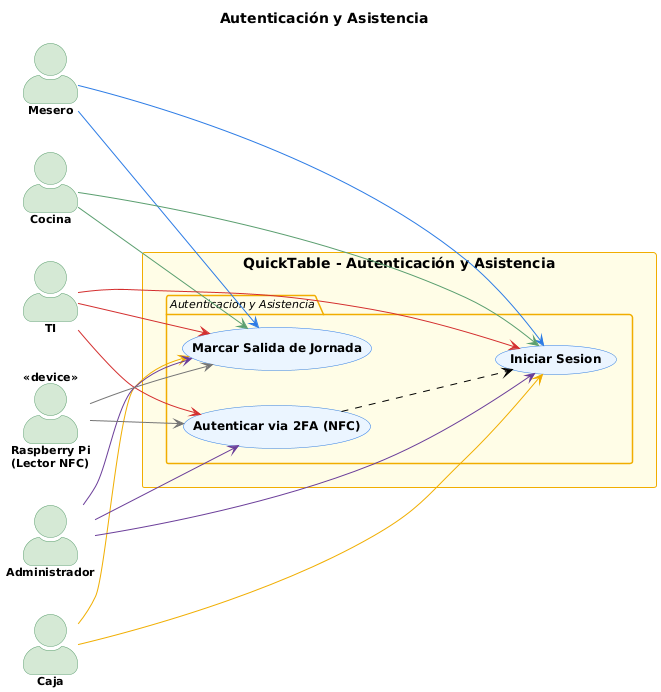
\includegraphics[width=0.8\textwidth]{imagenes/Autenticación y Asistencia.png}
	\caption{Casos de uso de autenticación y registro de asistencia (Realizado con PlantUML)}
	\label{fig:casos_uso_auth}
\end{figure}

La Figura~\ref{fig:casos_uso_auth} muestra los casos de uso relacionados con el inicio y cierre de jornada laboral, así como la autenticación mediante doble factor utilizando tarjetas NFC conectadas a una Raspberry Pi. En esta vista participan todos los roles del sistema, ya que cualquier empleado debe iniciar sesión, autenticarse y marcar la salida de su turno para que la aplicación pueda registrar las jornadas laborales y asociarlas con los pedidos realizados durante el día.

\begin{figure}[H]
	\centering
		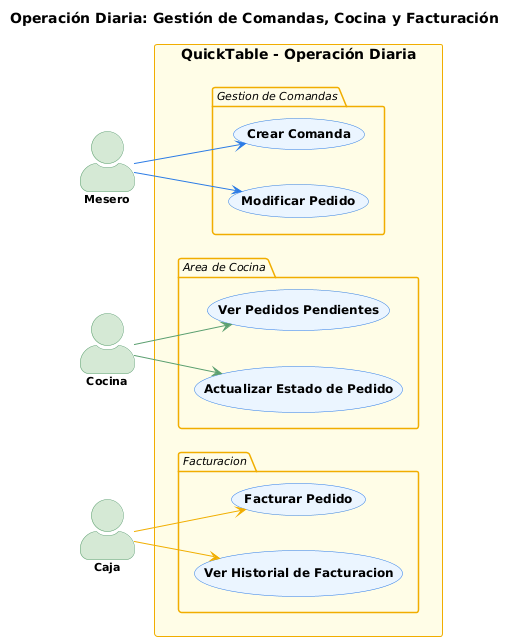
\includegraphics[width=0.75\textwidth]{imagenes/operacion diaria.png}
	\caption{Casos de uso de operación diaria: comandas, cocina y facturación (Realizado con PlantUML)}
	\label{fig:casos_uso_operacion}
\end{figure}

La Figura~\ref{fig:casos_uso_operacion} agrupa los casos de uso asociados a la operación diaria del restaurante: creación y edición de comandas por parte del mesero, gestión del estado de los pedidos en cocina y proceso de facturación en caja. Esta vista se centra en el flujo de una comanda desde que se registra en la mesa, pasa por la preparación en cocina y termina con la emisión de la factura y el cierre de la venta.

\begin{figure}[H]
	\centering
	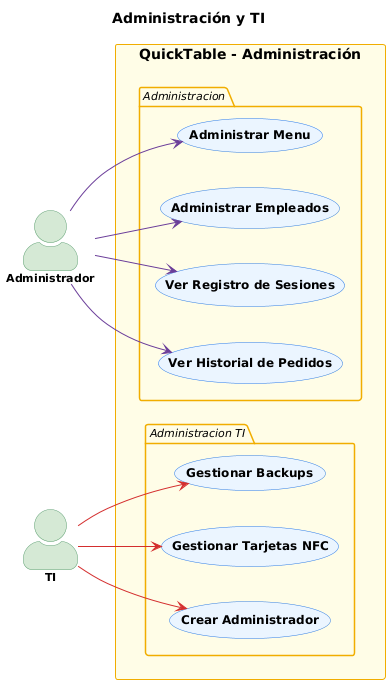
\includegraphics[width=0.6\textwidth]{imagenes/Administracion y ti.png}
	\caption{Casos de uso de administración del sistema y gestión TI (Realizado con PlantUML)}
	\label{fig:casos_uso_admin_ti}
\end{figure}

La Figura~\ref{fig:casos_uso_admin_ti} presenta los casos de uso exclusivos de los roles de Administrador y TI, incluyendo la gestión del menú, empleados, reportes e historial de pedidos, así como la administración de respaldos y de las tarjetas NFC. Estos casos de uso soportan las tareas de configuración, seguridad y mantenimiento del sistema, y están alineados con los módulos de administración y de gestión de tarjetas NFC implementados en la aplicación web.


\subsection{Requerimientos Funcionales (Criterios Given-When-Then)}

Para garantizar una evaluación objetiva durante la fase de pruebas, los requerimientos funcionales más críticos fueron redactados utilizando el formato \textit{Given-When-Then} (Dado-Cuando-Entonces), ampliamente utilizado en escenarios de \textit{Behavior-Driven Development} (BDD) y documentado en publicaciones recientes de IEEE sobre generación automática de casos de prueba a partir de escenarios BDD \cite{Zameni2023,ISO29148:2018}. En este enfoque, cada requerimiento se expresa como una tríada “Dado–Cuando–Entonces” que explicita la precondición, la acción del usuario o del sistema y el resultado esperado.

A continuación, se presentan los requerimientos funcionales principales agrupados por módulo operativo:



\begin{longtable}{|p{2.4cm}|p{4cm}|p{4cm}|p{4.5cm}|}
	\caption{Especificación de Requerimientos Funcionales (Módulos Operativos)} \label{tab:req_funcionales_operativos} \\
	\hline
	\textbf{ID / Módulo} & \textbf{Dado (Given)} & \textbf{Cuando (When)} & \textbf{Entonces (Then)} \\
	\hline
	\endfirsthead
	
	\hline
	\textbf{ID / Módulo} & \textbf{Dado (Given)} & \textbf{Cuando (When)} & \textbf{Entonces (Then)} \\
	\hline
	\endhead
	
	\hline
	\endfoot
	
	\hline
	\endlastfoot
	
	\textbf{RF-01} \newline Acceso al módulo de mesero
	&
	Existe una sesión válida y el usuario autenticado tiene el rol \texttt{Mesero}.
	&
	El usuario intenta ingresar al panel principal o al formulario de nuevo pedido.
	&
	El sistema permite el acceso a las vistas del módulo Mesero; si el rol no corresponde, redirige al \texttt{Index} correspondiente o no existe identificación válida en sesión, redirige al inicio de sesión.
	\\
	\hline
	
	\textbf{RF-02} \newline Creación de pedido
	&
	Un mesero autenticado se encuentra en la vista \texttt{NuevoPedido}, dispone de un número de mesa válido y selecciona al menos un ítem del menú.
	&
	El mesero confirma el pedido enviando la mesa, los ítems, sus cantidades y observaciones.
	&
	El sistema registra el pedido con sus detalles y cálculos financieros, y establece su estado inicial en \texttt{En Preparación}.
	\\
	\hline
	
	\textbf{RF-03} \newline Consulta y filtrado del menú
	&
	El mesero se encuentra creando o editando un pedido y el menú está disponible en la base de datos.
	&
	El usuario busca platos por nombre, filtra por categoría o ajusta cantidades desde la interfaz.
	&
	El sistema muestra los ítems del menú filtrados, permite aumentar o disminuir cantidades y conserva las observaciones digitadas para cada ítem seleccionado.
	\\
	\hline
	
	\textbf{RF-04} \newline Edición de pedido
	&
	Existe un pedido activo asociado al flujo del mesero y sus detalles están disponibles para modificación.
	&
	El mesero ingresa a \texttt{EditarPedido} y confirma cambios en cantidades, ítems u observaciones.
	&
	El sistema actualiza los detalles del pedido existente, recalcula los valores monetarios correspondientes y mantiene el pedido dentro del flujo operativo activo.
	\\
	\hline
	
	\textbf{RF-05} \newline Visualización de pedidos del mesero
	&
	El mesero ha iniciado sesión y existen pedidos activos registrados en el sistema.
	&
	El usuario consulta su panel de pedidos.
	&
	El sistema devuelve los pedidos asociados al mesero autenticado y permite además consultar pedidos de otros meseros mediante los endpoints dispuestos para esa visualización.
	\\
	\hline
	
	\textbf{RF-06} \newline Gestión de pedidos en cocina
	&
	Existen pedidos activos cuyo estado no ha finalizado el flujo de preparación y el usuario autenticado tiene rol \texttt{Cocina}.
	&
	Cocina consulta la vista de pedidos pendientes.
	&
	El sistema lista los pedidos con su número de mesa, identificador y detalles pendientes de preparación, mostrando solo las cantidades aún no preparadas y las observaciones registradas.
	\\
	\hline
	
	\textbf{RF-07} \newline Marcado de pedido listo
	&
	Un pedido activo se encuentra en estado \texttt{En Preparación} o \texttt{Editado} y está disponible en el módulo Cocina.
	&
	El usuario de cocina presiona la opción \texttt{Marcar como Listo}.
	&
	El sistema actualiza el pedido a estado \texttt{Listo}, registra la marca temporal correspondiente y deja el pedido disponible para seguimiento por parte del mesero y caja.
	\\
	\hline
	
	\textbf{RF-08} \newline Aceptación del pedido por el mesero
	&
	Existe un pedido previamente marcado como listo por cocina y visible para el mesero.
	&
	El mesero registra la aceptación del pedido.
	&
	El sistema almacena la fecha y hora de aceptación en el campo \texttt{MeseroAceptadoAt}, permitiendo medir tiempos operativos entre cocina y entrega.
	\\
	\hline
	
	\textbf{RF-09} \newline Consulta de pedidos activos en caja
	&
	El usuario autenticado tiene rol \texttt{Cajero} y existen pedidos activos en el sistema.
	&
	El cajero ingresa al módulo Caja y consulta los pedidos.
	&
	El sistema muestra cada pedido activo con mesa, mesero, estado, subtotal, IVA, total y detalle de productos, permitiendo distinguir visualmente si el pedido está listo o aún en preparación.
	\\
	\hline
	
	\textbf{RF-10} \newline Finalización y cobro del pedido
	&
	Existe un pedido activo seleccionado en caja y el cajero define propina y método de pago.
	&
	El cajero ejecuta la acción \texttt{FinalizarPedido}, indicando además efectivo recibido y cambio cuando aplica.
	&
	El sistema crea un registro en \texttt{HistorialPedido} con sus detalles, subtotal, IVA, total, propina, método de pago, efectivo recibido y cambio; posteriormente elimina el pedido de \texttt{PedidosActivos}.
	\\
	\hline
	
	\textbf{RF-11} \newline Generación de factura
	&
	Un pedido ya fue finalizado correctamente y existe su correspondiente registro en historial.
	&
	El sistema invoca la generación de la factura usando el identificador del pedido histórico.
	&
	El sistema construye la vista \texttt{Factura} con número de pedido, mesa, mesero, fecha, detalle de ítems, subtotal, IVA, propina, total final y método de pago.
	\\
	\hline
	
	\textbf{RF-12} \newline Consulta de historial de pedidos
	&
	Existen pedidos finalizados almacenados en \texttt{HistorialPedido} y el usuario tiene acceso al módulo Caja.
	&
	El cajero consulta el historial y aplica filtros por fecha, número de pedido o ID del mesero.
	&
	El sistema retorna los pedidos paginados del historial con su información general y detalle de productos, conservando los datos del cierre de venta para consulta posterior.
	\\
	\hline
	
\end{longtable}


\subsection{Requerimientos de Seguridad (2FA y Encriptación)}

Dado que uno de los pilares del proyecto es la seguridad y confidencialidad de la información, se establecieron requerimientos funcionales estrictos para el acceso administrativo y la protección de datos:

\begin{longtable}{|p{2.4cm}|p{4cm}|p{4cm}|p{4.5cm}|}
	\caption{Especificación de Requerimientos Funcionales de Seguridad}
	\label{tab:req_funcionales_seguridad} \\
	\hline
	\textbf{ID / Módulo} & \textbf{Dado (Given)} & \textbf{Cuando (When)} & \textbf{Entonces (Then)} \\
	\hline
	\endfirsthead
	
	\hline
	\textbf{ID / Módulo} & \textbf{Dado (Given)} & \textbf{Cuando (When)} & \textbf{Entonces (Then)} \\
	\hline
	\endhead
	
	\hline
	\endfoot
	
	\hline
	\endlastfoot
	
	\textbf{RS-01} \newline Provisión de tarjeta para administrador
	&
	Existe un administrador creado o en proceso de habilitación dentro del módulo de gestión de tarjetas.
	&
	Se solicita registrar o asociar una tarjeta NFC al flujo de acceso administrativo.
	&
	El sistema registra la tarjeta, protege el identificador correspondiente y deja disponible el factor físico necesario para el proceso de validación administrativa.
	\\
	\hline
	
	\textbf{RS-02} \newline Protección de contraseñas
	&
	Se crea un usuario o se actualiza una contraseña en el sistema.
	&
	La contraseña debe almacenarse para autenticaciones futuras.
	&
	El sistema protege la contraseña mediante hashing BCrypt y utiliza el mecanismo de verificación correspondiente cuando el usuario intenta autenticarse.
	\\
	\hline
	
	\textbf{RS-03} \newline Autenticación por credenciales
	&
	Existe un empleado registrado con nombre de usuario y contraseña almacenada.
	&
	El usuario ingresa sus credenciales en el formulario de inicio de sesión.
	&
	El sistema busca el empleado por nombre, valida la contraseña protegida y solo permite continuar el proceso de acceso cuando las credenciales son correctas.
	\\
	\hline
	
	\textbf{RS-04} \newline Doble factor exclusivo para administrador
	&
	Un usuario con rol de \texttt{administrador} ya superó la validación inicial de usuario y contraseña, y existe un proceso de segundo factor asociado a su autenticación.
	&
	El sistema recibe la confirmación del segundo factor mediante el flujo de \texttt{Confirmar2FA} y consulta su estado con \texttt{Check2FA}.
	&
	El sistema concede el acceso administrativo únicamente cuando el segundo factor ha sido confirmado correctamente; este control reforzado aplica al administrador.
	\\
	\hline
	
	\textbf{RS-05} \newline Validación de sesión para hardware
	&
	Existe un código de sesión generado para un flujo de validación con dispositivo o tarjeta NFC.
	&
	El cliente o dispositivo envía el código de sesión a los mecanismos de validación definidos para administrador o empleado.
	&
	El sistema verifica el formato y la vigencia del código, y autoriza la operación solo si la sesión correspondiente es válida.
	\\
	\hline
	
	\textbf{RS-06} \newline Control de acceso por rol
	&
	Existe una sesión iniciada o un usuario intenta acceder a un módulo protegido.
	&
	El usuario intenta ingresar a una vista o acción restringida a un rol específico.
	&
	El sistema valida el rol almacenado en sesión y permite el acceso únicamente al módulo autorizado; en caso contrario, redirige al inicio de sesión o rechaza la solicitud.
	\\
	\hline
	
	\textbf{RS-07} \newline Gestión segura de sesión
	&
	Un usuario autenticado inicia o mantiene una sesión activa en la aplicación.
	&
	El sistema crea, conserva o finaliza la sesión del usuario.
	&
	El sistema registra conexión y desconexión, configura la sesión mediante cookie \texttt{HttpOnly}, aplica expiración por inactividad y limpia procesos pendientes al cerrar sesión.
	\\
	\hline
	
\end{longtable}


\subsection{Requerimientos No Funcionales}

Además de las funcionalidades, el diseño del sistema debió contemplar restricciones técnicas que garantizaran su viabilidad operativa, seguridad, mantenibilidad y bajo costo de implementación, considerando las capacidades tecnológicas habituales de los restaurantes PYME.

\begin{itemize}
	\item \textbf{Multiplataforma:} La interfaz de usuario debe ser accesible y responsiva desde dispositivos móviles (smartphones y tablets) y computadores de escritorio mediante navegadores web modernos, evitando la necesidad de instalar aplicaciones nativas.
	
	\item \textbf{Despliegue Local (Intranet):} El sistema debe operar sobre una red local del establecimiento, sin depender de una conexión permanente a internet para ejecutar sus funciones principales.
	
	\item \textbf{Tiempos de Respuesta:} Las operaciones de consulta, registro y actualización de comandas deben ejecutarse con tiempos de respuesta suficientemente bajos para no afectar el flujo operativo del restaurante, idealmente en menos de 2 segundos por transacción.
	
	\item \textbf{Optimización de Recursos:} El backend y la base de datos deben poder ejecutarse sobre hardware de gama de entrada, con el fin de mantener bajos los costos de adopción para pequeñas y medianas empresas.
	
	\item \textbf{Seguridad de Sesión:} El sistema debe administrar sesiones de usuario con mecanismos que reduzcan accesos no autorizados, incluyendo expiración por inactividad y uso de cookies seguras de sesión.
	
	\item \textbf{Protección de Datos Sensibles:} La información sensible, como credenciales y datos asociados a mecanismos de autenticación, debe almacenarse utilizando técnicas de protección criptográfica apropiadas.
	
	\item \textbf{Respaldo y Recuperación:} El sistema debe permitir la generación y restauración de copias de seguridad para proteger la información operativa frente a fallos del sistema o pérdida de datos.
	
	\item \textbf{Mantenibilidad:} La solución debe conservar una estructura modular que facilite la corrección de errores, la evolución del sistema y la incorporación de nuevas funcionalidades sin afectar los componentes ya implementados.
	
	\item \textbf{Trazabilidad Operativa:} El sistema debe registrar eventos relevantes de acceso y cierre de sesión para facilitar el control administrativo y el seguimiento de la operación diaria.
\end{itemize}




%\subsection{Casos de Uso}
% Aquí puedes incluir un diagrama de casos de uso general y explicar los roles: Administrador, Mesero, Cocina, Caja y TI.
% Ejemplo de figura para el diagrama de casos de uso:
% \begin{figure}[H]
	%     \centering
	%     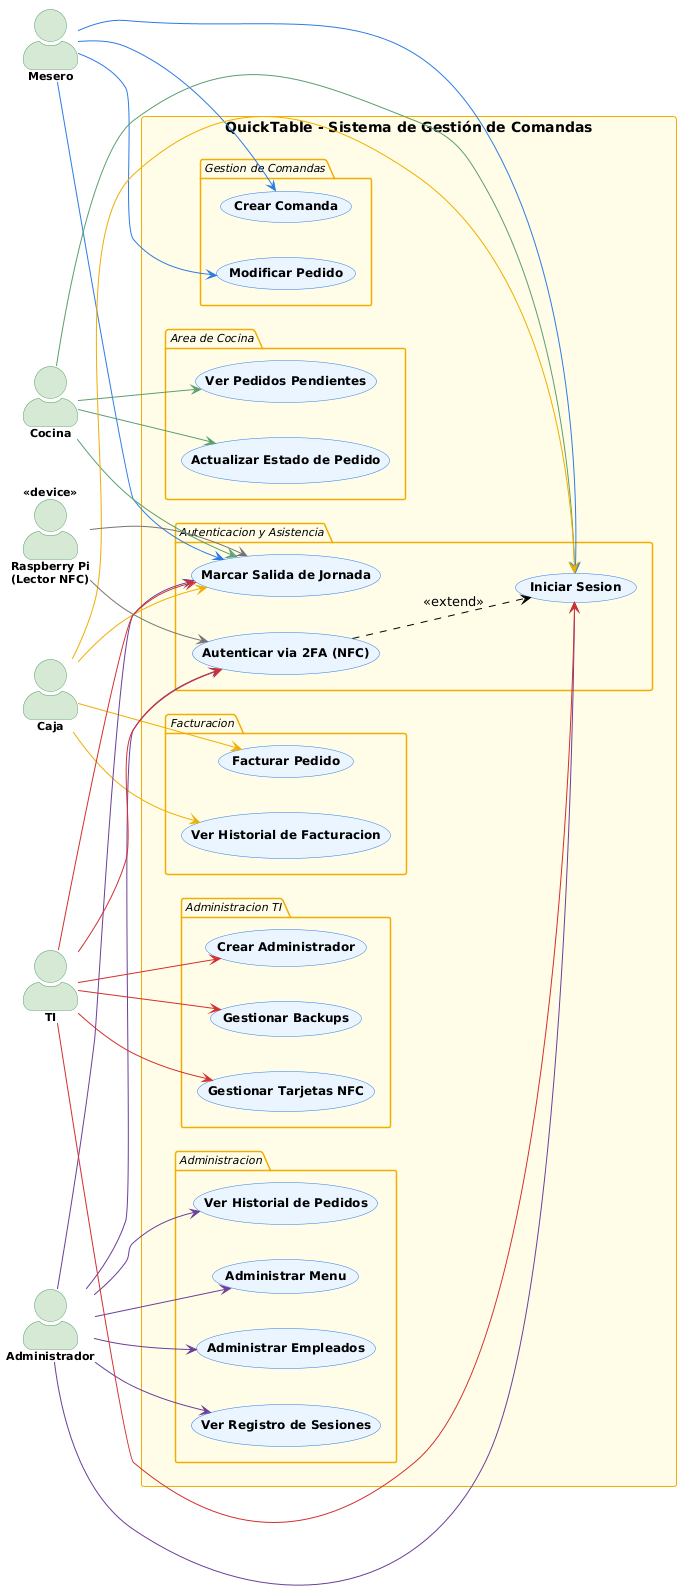
\includegraphics[width=0.8\textwidth]{casos_uso.png}
	%     \caption{Diagrama general de casos de uso del sistema}
	%     \label{fig:casos_uso}
	% \end{figure}

\subsection{Arquitectura General del Sistema}
Para el desarrollo de la aplicación se implementó una arquitectura cliente-servidor basada en el modelo de tres capas: Presentación, Lógica de Negocio y Datos. Esta estructura garantiza la separación de responsabilidades, facilitando la escalabilidad, el mantenimiento del código y la seguridad del sistema. El patrón arquitectónico principal utilizado fue el Modelo-Vista-Controlador (MVC), adaptado mediante la tecnología Razor Pages de .NET 8, la cual encapsula el modelo y el controlador en una clase unificada (\texttt{PageModel}) vinculada directamente a su respectiva vista, optimizando el flujo de trabajo en aplicaciones orientadas a páginas.

La arquitectura general se compone de los siguientes elementos:

\begin{itemize}
	\item \textbf{Capa de Presentación (Frontend):} Desarrollada utilizando HTML5, CSS3, JavaScript y el framework Bootstrap. La interfaz de usuario toma como base estructural la plantilla AdminLTE, la cual fue extendida y fuertemente personalizada para adaptar la apariencia a las necesidades visuales y operativas del sistema en dispositivos móviles y de escritorio.
	\item \textbf{Capa de Aplicación (Backend):} Construida con el framework .NET 8 en el lenguaje C\#. Es responsable de procesar las peticiones HTTP, ejecutar las reglas de negocio y gestionar la comunicación con el módulo de hardware RFID mediante Endpoints de API tipo REST.
	\item \textbf{Capa de Datos:} Implementada sobre el motor de base de datos relacional Microsoft SQL Server, utilizando el ORM Entity Framework 6 (EF6) para garantizar una comunicación segura y transaccional.
	\item \textbf{Módulo de Seguridad (Hardware):} Compuesto por una Raspberry Pi interactuando con un lector NFC RFID-RC522, el cual actúa como un cliente independiente para la validación física del administrador en el esquema de doble factor de autenticación (2FA).
\end{itemize}

% diagrama de bloques
\begin{figure}[H]
	\centering
	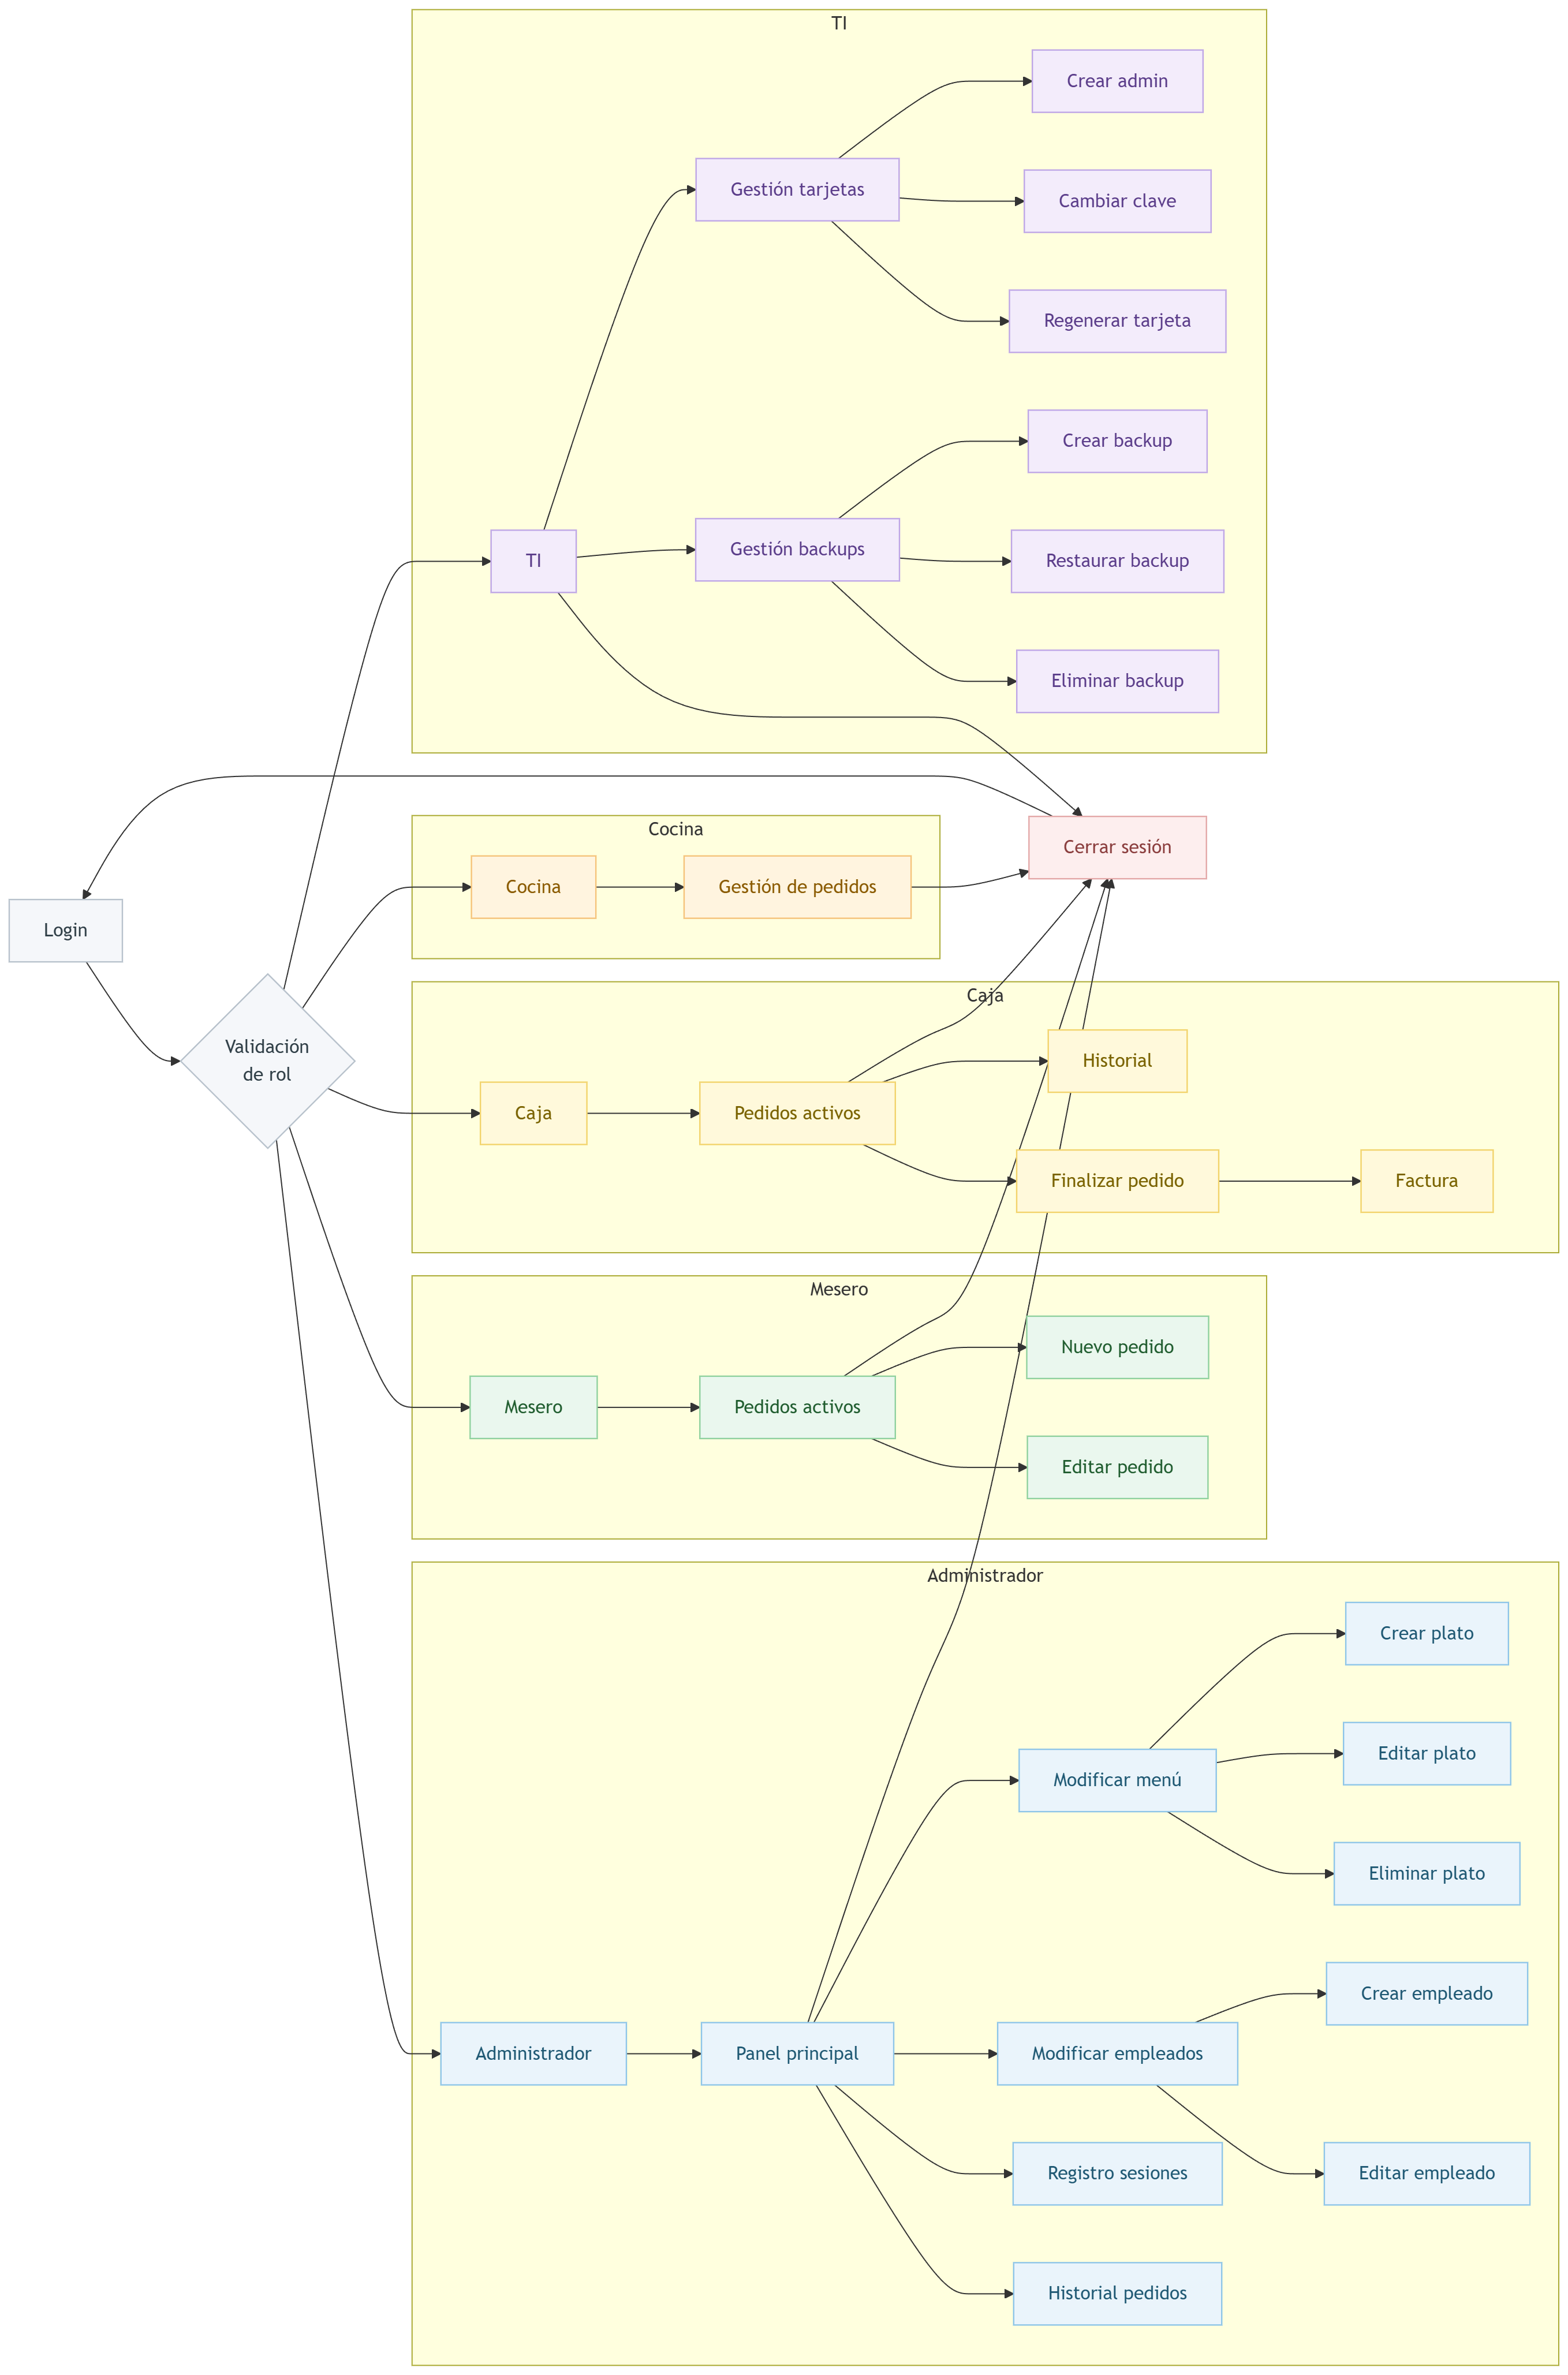
\includegraphics[width=0.9\textwidth]{imagenes/arquitectura_bloques.png}
	\caption{Diagrama de bloques de la arquitectura del sistema}
	\label{fig:arquitectura_bloques}
\end{figure}


\section{Diseño e Implementación de la Base de Datos}

El diseño de la base de datos se estructuró para soportar las operaciones críticas del restaurante de manera transaccional, garantizando la integridad referencial y minimizando la redundancia de datos. Se optó por el motor Microsoft SQL Server debido a su robustez, soporte nativo de encriptación y excelente integración con el ecosistema de desarrollo de Microsoft.

\subsection{Modelo Entidad-Relación}

El esquema de la base de datos consta de tablas interrelacionadas que representan las entidades fundamentales del negocio y los mecanismos de seguridad. Entre las entidades principales se encuentran:

\begin{itemize}
	\item \textbf{Empleados:} Almacena las credenciales protegidas (mediante hashing BCrypt) de los usuarios, sus datos personales, el UID asociado (si aplica) y el rol asignado dentro del sistema (Admin, Mesero, Cocina, Cajero).
	\item \textbf{MenuItems (Menú):} Contiene el catálogo de productos disponibles, sus descripciones, categorías y precios, permitiendo la construcción dinámica de los pedidos.
	\item \textbf{PedidosActivos e ItemDetalle:} Tablas transaccionales encargadas de almacenar el encabezado de la comanda en curso (fecha, mesero, mesa, totales y estado de preparación) y los ítems individuales con sus cantidades y observaciones, respectivamente.
	\item \textbf{HistorialPedidos e HistorialDetalle:} Entidades destinadas a la persistencia de las comandas ya facturadas y finalizadas, garantizando la inmutabilidad de los datos históricos de ventas y facturación.
	\item \textbf{TarjetasRC:} Tabla dedicada a la seguridad por hardware, que almacena el UID físico de las tarjetas NFC y gestiona la asignación activa a los usuarios administradores.
	\item \textbf{RegistroSesiones y Codigos2FA:} Entidades de auditoría y control de acceso. La primera registra las horas de conexión y desconexión de los empleados para el control de asistencia, mientras que la segunda gestiona de forma temporal los tokens para la autenticación de doble factor.
\end{itemize}

 \begin{figure}[H] 
	 	\centering
	 	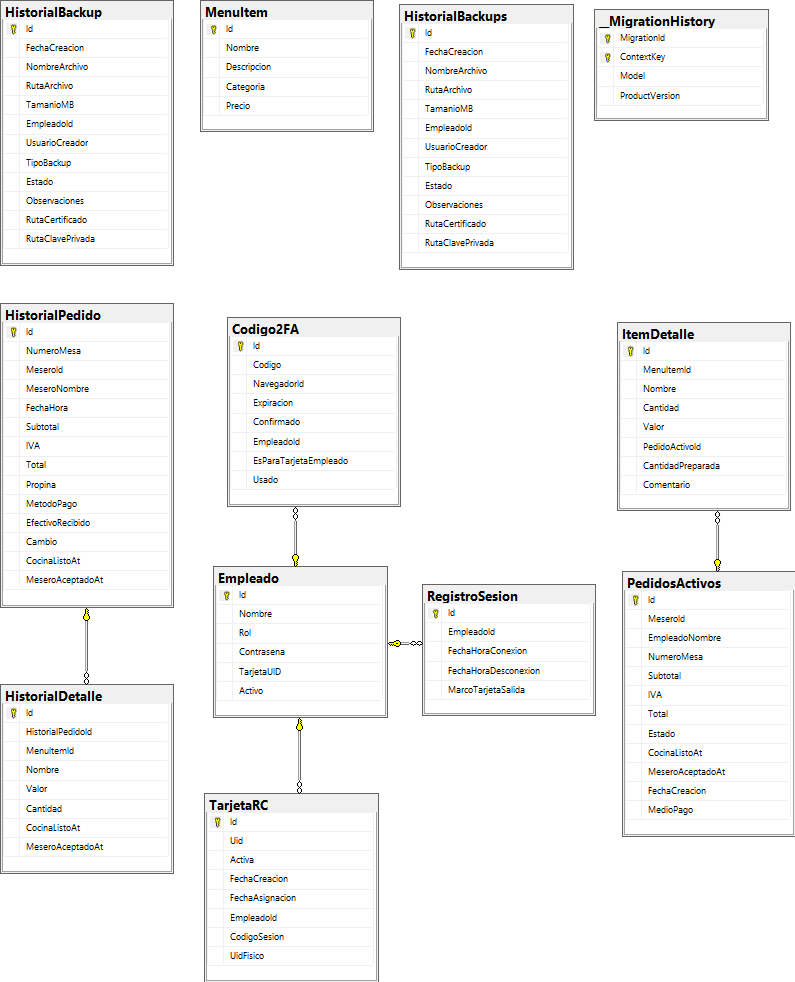
\includegraphics[width=0.95\textwidth]{imagenes/diagrama_mer.png}
	 	\caption{Modelo Entidad-Relación de la base de datos (Creado en SMSS 20)}
	 	\label{fig:diagrama_mer}
	 \end{figure}

Como se observa en la Figura \ref{fig:diagrama_mer}, el modelo de datos fue diseñado siguiendo un enfoque relacional normalizado que separa claramente la operación en tiempo real de la persistencia histórica. La entidad central del sistema es \textbf{Empleado}, la cual establece una relación de 'uno a muchos' tanto con los \textbf{PedidosActivos} como con el \textbf{RegistroSesion}, permitiendo la trazabilidad de qué usuario (Mesero) crea cada comanda y en qué horarios labora el personal. Asimismo, mantiene una relación opcional de 'uno a uno' con la tabla \textbf{TarjetaRC}, utilizada exclusivamente para vincular credenciales físicas NFC a los perfiles con rol de Administrador.

El flujo transaccional del restaurante se maneja a través de dos estructuras gemelas: una para la operación en curso y otra para el archivo histórico. Un \textbf{PedidoActivo} actúa como entidad cabecera que se relaciona de 'uno a muchos' con \textbf{ItemDetalle}, donde cada detalle hace referencia mediante llave foránea al producto específico en la tabla \textbf{MenuItem}. Una vez que el Cajero procesa el pago y finaliza la orden, la integridad de los datos se garantiza migrando la información hacia las entidades \textbf{HistorialPedido} e \textbf{HistorialDetalle}. Esta separación arquitectónica evita la sobrecarga de la tabla de pedidos activos, garantizando tiempos de respuesta rápidos (menores a 2 segundos) para el personal de Meseros y Cocina, mientras se conservan los datos inmutables de facturación para consultas administrativas.

\subsection{Implementación con Entity Framework 6}
La arquitectura de persistencia de datos del sistema fue implementada utilizando Entity Framework 6 (EF6) bajo el ecosistema de .NET 8. Se optó por EF6 debido a su alta madurez y estabilidad a nivel empresarial. Al contar con una extensa documentación y un motor de persistencia rigurosamente probado contra fallos transaccionales, se reduce la curva de aprendizaje para futuros mantenimientos, alineándose con el objetivo de ofrecer una solución escalable y de bajo costo para las PYMES.

Para gestionar la interacción con la base de datos, el sistema define un contexto principal denominado \texttt{SistemaQuickTableContext}, el cual hereda de la clase base \texttt{DbContext}. La persistencia se estructura bajo los siguientes principios:

\begin{itemize}
	\item \textbf{Mapeo Objeto-Relacional Consolidado:} Las tablas de SQL Server se representan directamente mediante entidades (clases) ubicadas en el directorio \texttt{Dominio} (ej. \texttt{PedidoActivo}, \texttt{ItemDetalle}). El contexto administra el estado de estas entidades a través de colecciones \texttt{DbSet<T>}, garantizando que las modificaciones en la lógica de negocio se traduzcan de manera íntegra a la base de datos.
	\item \textbf{Gestión Segura de Conexiones:} La cadena de conexión al motor SQL Server se inyecta dinámicamente desde el archivo de configuración \texttt{appsettings.json}. Esta separación aísla las credenciales de acceso del código fuente principal, cumpliendo con las buenas prácticas de seguridad informática.
	\item \textbf{Abstracción de Consultas con LINQ:} Las operaciones CRUD ejecutadas por los diferentes módulos no emplean sentencias SQL estáticas. En su lugar, se utiliza \textit{Language Integrated Query} (LINQ), lo cual mitiga por diseño las vulnerabilidades de inyección SQL y optimiza la legibilidad del código al expresar reglas de negocio en lenguaje nativo C\#.
\end{itemize}


\section{Implementación de la Solución Web}

El núcleo central del sistema fue desarrollado como una aplicación web robusta, diseñada para centralizar la comunicación entre las áreas del restaurante y eliminar las ineficiencias del papel. El desarrollo se fundamentó en el ecosistema de Microsoft, utilizando .NET 8 y el patrón arquitectónico MVC (Modelo-Vista-Controlador) adaptado mediante el enfoque de \textit{Razor Pages}.

\subsection{Interfaz de Usuario (Frontend y Personalización visual)}

Como se estableció en el diseño arquitectónico, la capa de presentación toma como base estructural el framework \textbf{AdminLTE} (soportado por Bootstrap). Sin embargo, su implementación no se limitó al uso genérico de la plantilla; esta fue sometida a una \textbf{reestructuración y personalización profunda mediante hojas de estilo propias (CSS)}. El objetivo de esta sobreescritura de estilos fue transformar un panel de control administrativo estándar en una interfaz operativa ágil, adaptada específicamente a las condiciones físicas del sector gastronómico.

Esta implementación personalizada aportó las siguientes características técnicas al proyecto:

\begin{itemize}
	\item \textbf{Diseño Responsivo y Optimización Táctil:} Si bien la estructura de grillas de Bootstrap garantiza la adaptabilidad a diferentes resoluciones, el CSS personalizado se enfocó en ampliar las áreas de interacción (botones, selectores de cantidad y tarjetas de menú). Esto es vital para facilitar la precisión táctil en los \textit{smartphones} de los meseros y evitar toques accidentales durante operaciones rápidas.
	\item \textbf{Minimalismo y Contraste Visual:} Se sobrescribieron los estilos predeterminados de AdminLTE para ocultar elementos modulares innecesarios (como menús laterales complejos) en las vistas operativas. Asimismo, se implementó una paleta de colores de alto contraste que permite a los cocineros y cajeros identificar visualmente y a distancia el estado de un pedido (por ejemplo, alertas visuales para comandas en espera prolongada o listas para entrega).
	\item \textbf{Interactividad Asíncrona:} Para complementar el diseño visual, se integró JavaScript (junto con librerías como jQuery y DataTables) en las vistas de Razor Pages. Esto permitió habilitar acciones dinámicas sin necesidad de recargar la página completa, optimizando tiempos muertos al momento de filtrar el menú o actualizar el estado de preparación de un plato.
\end{itemize}


\subsection{Lógica de Negocio y Módulos .NET 8 (Razor Pages)}
El backend de la aplicación gestiona la lógica de negocio a través del enfoque de Razor Pages, el cual agrupa los controladores y las vistas en un diseño orientado a páginas (\textit{Page-Focused}), resultando en un código más organizado y fácil de mantener que el MVC tradicional para este tipo de aplicaciones. 

El sistema fue segmentado en cinco módulos principales, protegidos por un sistema de autorización basado en reclamaciones (\textit{Claims}) que restringe el acceso según el rol del empleado autenticado:

\begin{itemize}
	\item \textbf{Módulo de Meseros:} Implementa el modelo \texttt{PageModel} para recibir peticiones HTTP POST con objetos JSON que contienen los arreglos de productos. El controlador procesa la lógica matemática de impuestos y subtotales en el servidor y ejecuta la persistencia inicial del registro en la tabla \texttt{PedidosActivos}.
	\item \textbf{Módulo de Cocina:} Funciona mediante consultas asíncronas periódicas (AJAX) que interrogan a la base de datos para extraer dinámicamente los registros con estado pendiente. A través de Endpoints específicos, permite la actualización de estados y marcas temporales sin necesidad de recargar el DOM completo.
	\item \textbf{Módulo de Caja:} Su controlador gestiona el ciclo de vida final del objeto pedido. Tras la confirmación del pago mediante peticiones asíncronas, el sistema ejecuta la lógica transaccional de migración de datos, trasladando la información desde las tablas operativas (\texttt{PedidosActivos}) hacia las entidades inmutables del esquema (\texttt{HistorialPedidos}).
	\item \textbf{Módulos de Administración y TI:} Exponen las interfaces de configuración del CRUD de inventarios y empleados, y gestionan los algoritmos criptográficos (hashing de credenciales). Además, orquestan la comunicación externa exponiendo los Endpoints REST de la API que interactúan con la Raspberry Pi para la verificación de tarjetas NFC.
\end{itemize}


% Descomentar y ajustar cuando tengas pantallazos del sistema
% \begin{figure}[H]
	%     \centering
	%     \includegraphics[width=0.85\textwidth]{imagenes/interfaz_mesero.png}
	%     \caption{Interfaz de usuario del módulo de mesero (diseño responsivo)}
	%     \label{fig:interfaz_mesero}
	% \end{figure}

\subsection{Análisis Visual de la Interfaz Implementada}

Para validar el cumplimiento de los requerimientos de usabilidad y la correcta aplicación de los estilos CSS personalizados sobre AdminLTE, se desarrollaron esquemas visuales comentados a partir de las interfaces finales del sistema. Estos diagramas evidencian las decisiones de diseño enfocadas en la operación rápida y la visualización en diferentes dispositivos (Figura \ref{fig:interfaz_mesero_anotada} y Figura \ref{fig:interfaz_cocina_anotada}).

En la vista destinada al personal de servicio (Meseros), se priorizó el diseño \textit{Mobile-First}, maximizando las áreas táctiles para la selección de platos y el ajuste de cantidades. Se implementaron tarjetas (\textit{cards}) individuales para cada ítem del menú, facilitando su lectura en pantallas reducidas.

\begin{figure}[H]
	\centering
	% Sugerencia: Una imagen de un celular mostrando la toma de pedidos con flechas apuntando a los botones grandes.
	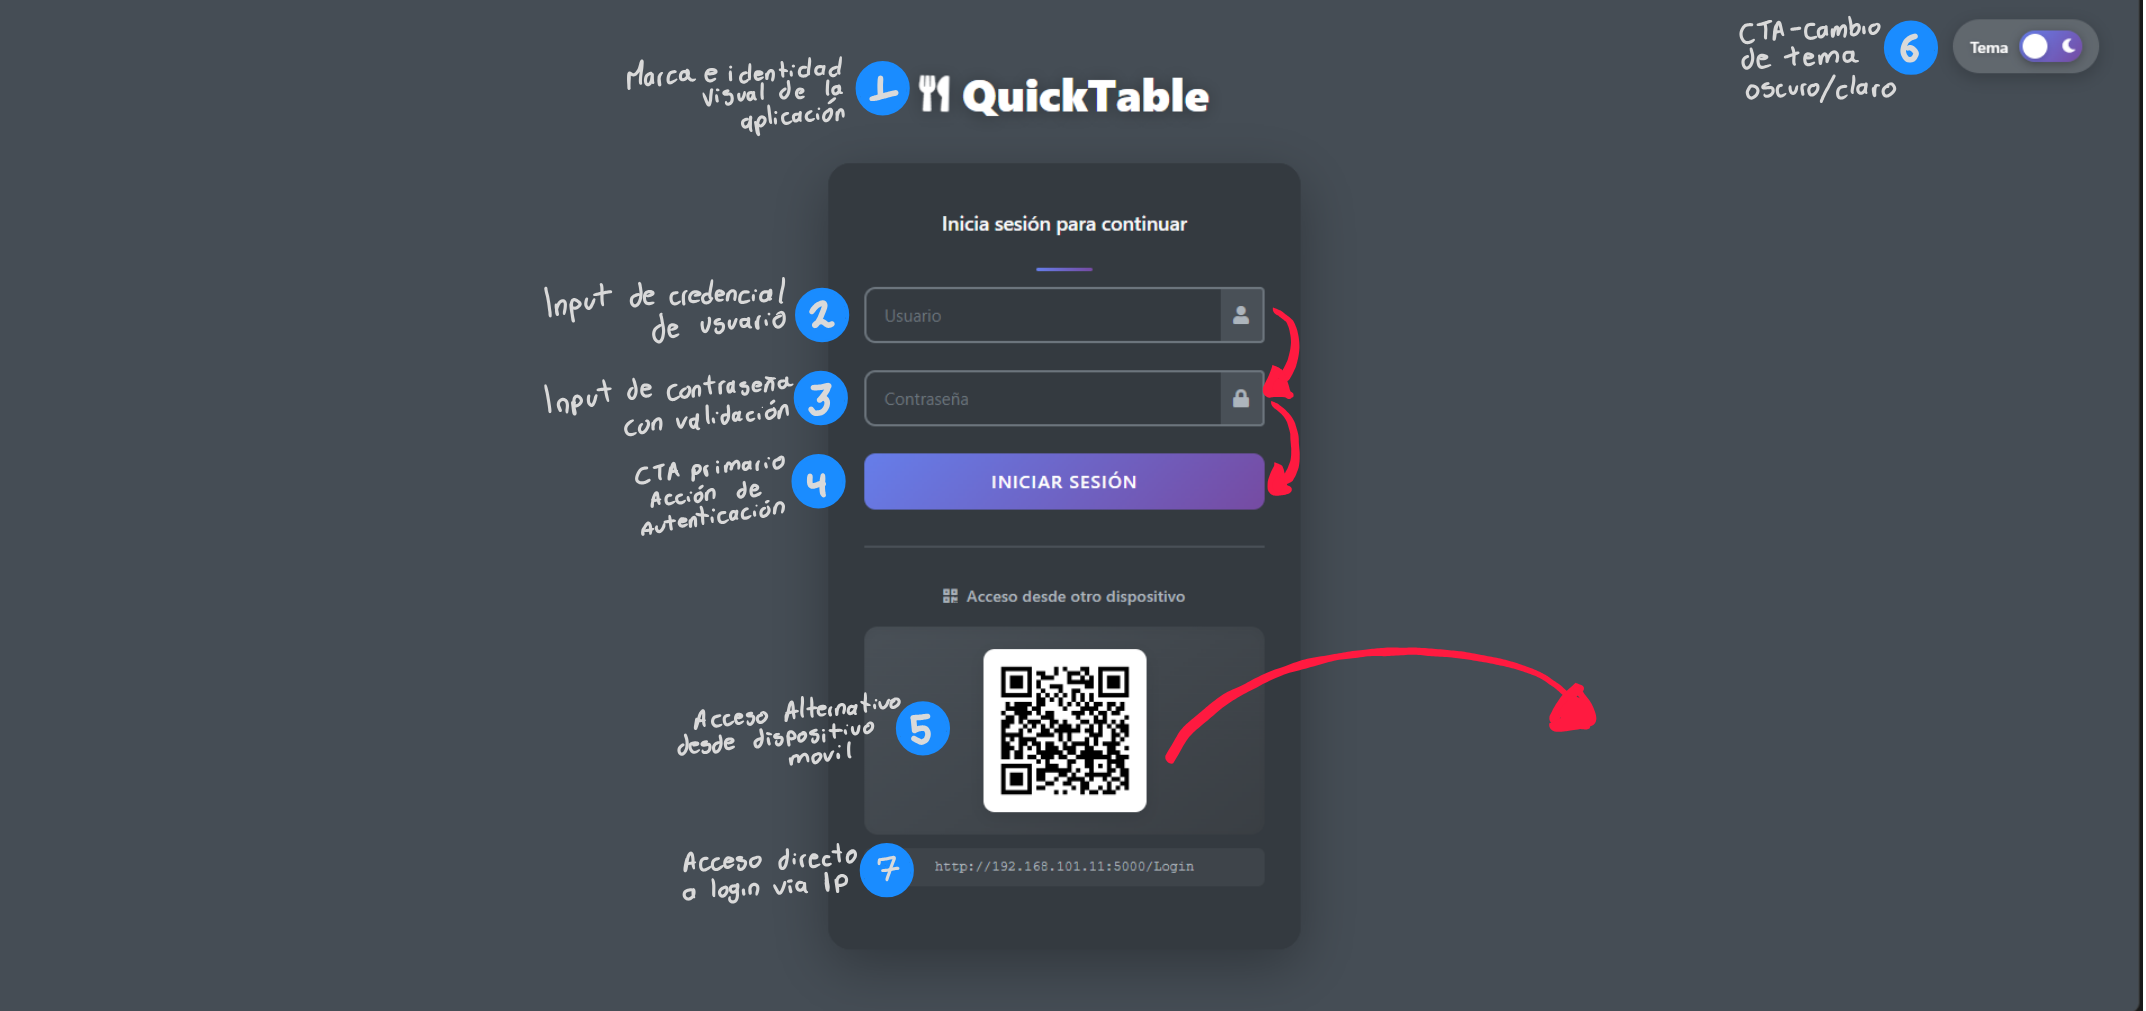
\includegraphics[width=0.85\textwidth]{imagenes/mockup_mesero.png} 
	\caption{CAMBIAR.}
	\label{fig:interfaz_mesero_anotada}
\end{figure}

Por otro lado, la vista del módulo de Cocina fue diseñada para su visualización en pantallas de formato horizontal (monitores o tablets en formato apaisado). Como se observa en la distribución de los componentes, la interfaz minimiza la interacción física requerida por parte del cocinero, mostrando la información estructurada por comandas entrantes y utilizando un código de colores de alto contraste para identificar el estado de preparación de los alimentos.

\begin{figure}[H]
	\centering
	% Sugerencia: Una imagen de la pantalla de cocina (monitor) con notas sobre los colores de estado y el botón "Marcar Listo".
	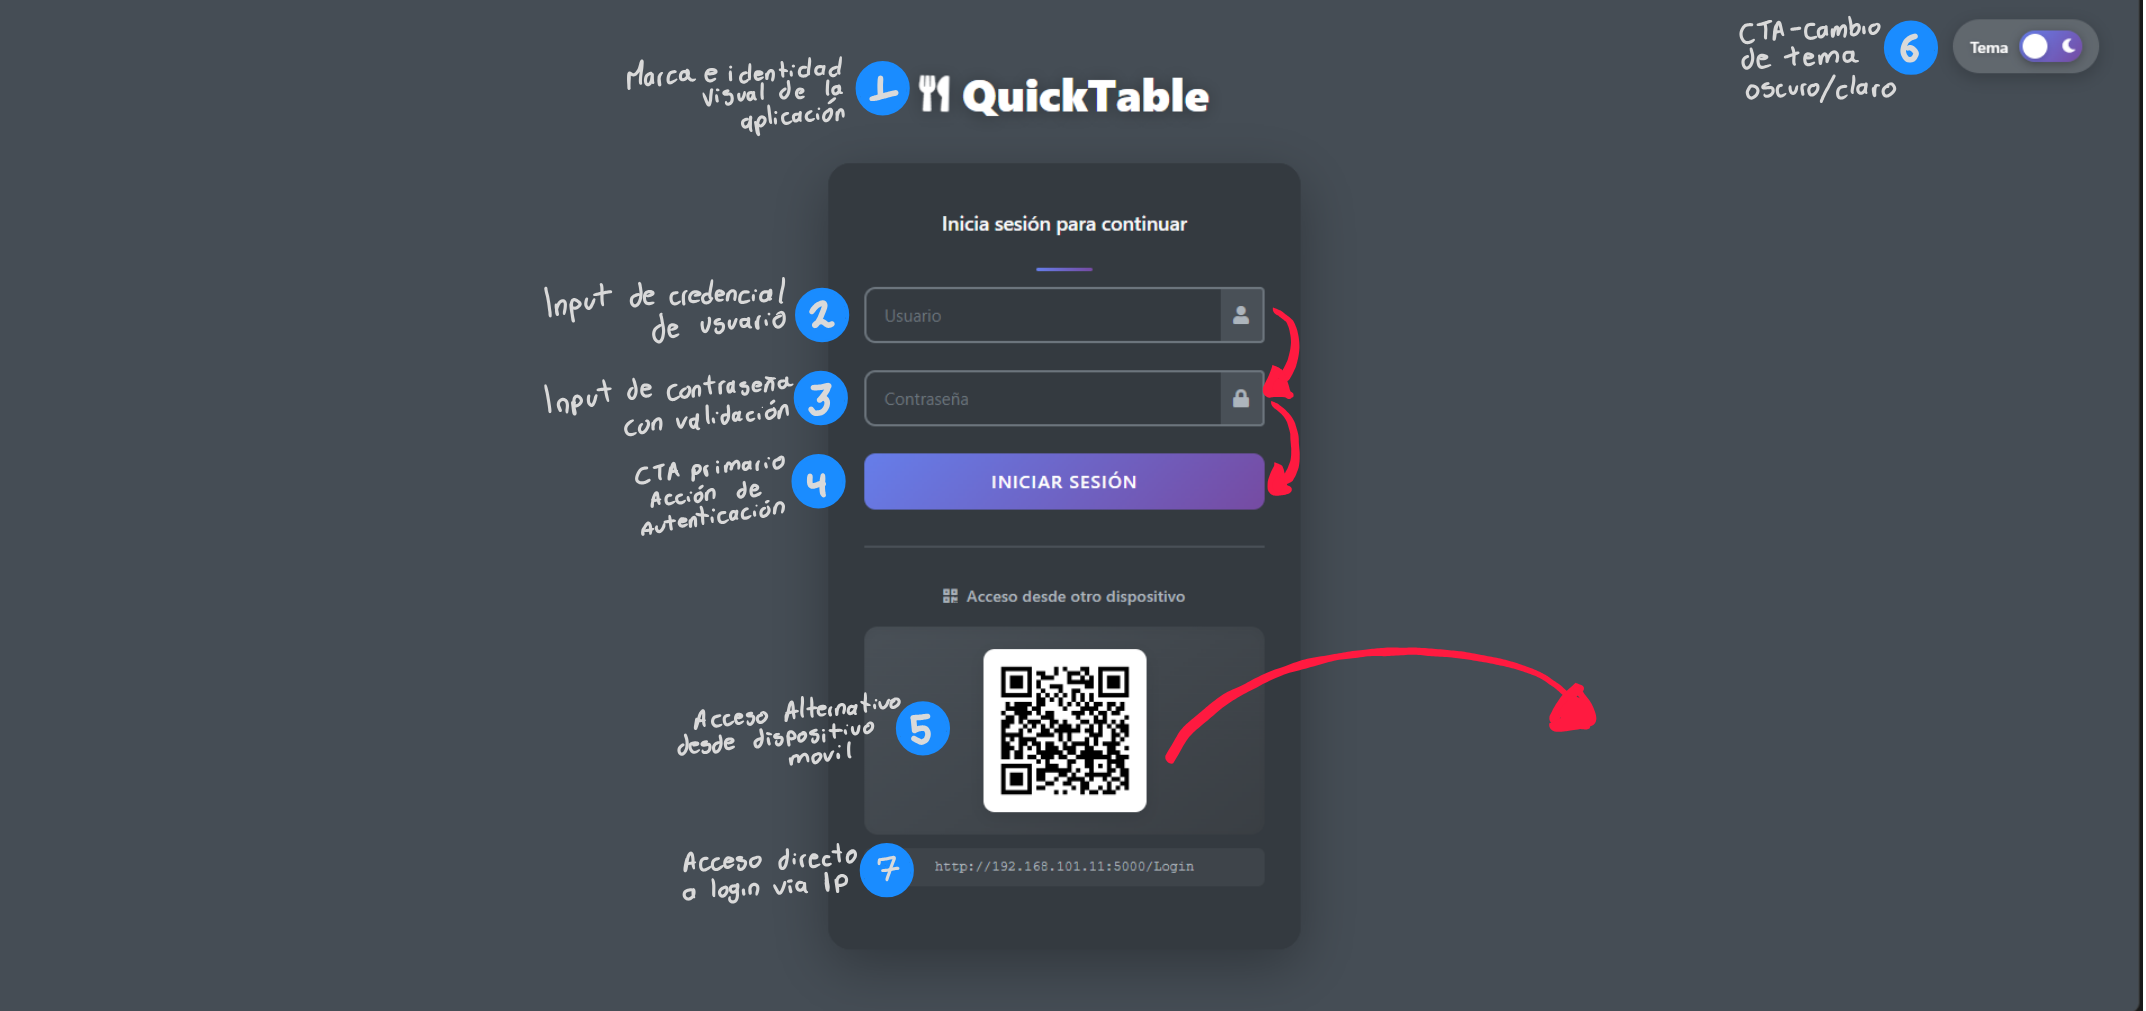
\includegraphics[width=0.9\textwidth]{imagenes/mockup_mesero.png} 
	\caption{CAMBIAR}
	\label{fig:interfaz_cocina_anotada}
\end{figure}





\section{Implementación del Módulo de Seguridad por Hardware (2FA Local)}

En el contexto del desarrollo de aplicaciones web contemporáneas, la implementación de mecanismos de Autenticación de Doble Factor (2FA) se ha estandarizado mediante el uso de servicios basados en la nube, tales como el envío de tokens por SMS, correos electrónicos o aplicaciones generadoras de códigos (ej. Microsoft Authenticator). Sin embargo, en el marco de este proyecto, dichos métodos presentan un obstáculo técnico restrictivo: \textbf{su dependencia de una conexión activa a Internet}.

Dado que uno de los requerimientos no funcionales prioritarios del sistema es garantizar su funcionamiento ininterrumpido sobre una red local (Intranet) con el fin de reducir los costos operativos mensuales para el establecimiento, se descartó la integración de sistemas 2FA en la nube. En su lugar, se diseñó e implementó un módulo de seguridad por hardware basado en tecnología NFC (\textit{Near Field Communication}). Este enfoque añade una capa de seguridad basada en un factor físico de posesión ('algo que el usuario tiene'), garantizando la presencia in situ del administrador al momento de autorizar accesos críticos, operando de manera 100\% \textit{offline} e integrándose de forma nativa con el servidor .NET 8.

\subsection{Arquitectura y Configuración del Hardware}

El dispositivo de validación física actúa como un cliente independiente dentro de la red local del restaurante. Su arquitectura de hardware se compone de dos elementos principales:

\begin{itemize}
	\item \textbf{Unidad de Procesamiento:} Se utilizó una placa \textit{Raspberry Pi 3 Model B v1.2}, la cual ofrece conectividad de red local (Wi-Fi/Ethernet) y los pines de propósito general (GPIO) necesarios para la interacción con periféricos externos.
	\item \textbf{Lector RFID/NFC:} Se integró el módulo \textit{RFID-RC522}, que opera a una frecuencia de 13.56 MHz. Este sensor fue seleccionado por su bajo costo, bajo consumo energético y alta fiabilidad en entornos comerciales.
\end{itemize}

La comunicación entre la Raspberry Pi y el lector RC522 se estableció mediante el protocolo de comunicación síncrona \textbf{SPI} (\textit{Serial Peripheral Interface}). Se configuraron los pines físicos correspondientes (MOSI, MISO, SCK, SDA y RST) para garantizar una transmisión de datos rápida y libre de interferencias al momento de leer el identificador único (UID) de las tarjetas asignadas a los administradores.

\subsection{Desarrollo del Cliente Python e Interfaz Gráfica (Tkinter)}
Para gobernar el comportamiento del hardware de validación física, se desarrolló un script en Python 3 que se ejecuta localmente en la Raspberry Pi. Este lenguaje fue seleccionado por su alta compatibilidad con el sistema operativo (Raspberry Pi OS) y la madurez de sus librerías para la manipulación de los puertos GPIO.

Para optimizar la interacción del usuario sin requerir periféricos externos como teclados o ratones, el dispositivo fue dotado de una Interfaz Gráfica de Usuario (GUI) orientada a pantallas táctiles, desarrollada con la librería estándar \texttt{Tkinter}. El diseño presenta un teclado numérico renderizado en pantalla (\textit{numpad}), permitiendo al administrador digitar un código de sesión dinámico temporal que vincula la lectura física de la tarjeta NFC con el intento de inicio de sesión en el navegador web.

El funcionamiento interno del programa se apoya en la integración concurrente de tres librerías fundamentales:
\begin{enumerate}
	\item \textbf{Tkinter (GUI):} Encargada de la construcción visual y de capturar las pulsaciones del usuario en la pantalla táctil mediante su bucle principal de eventos (\textit{mainloop}).
	\item \textbf{mfrc522 (Hardware):} Librería especializada que inicializa la comunicación por el bus SPI, activa el campo electromagnético del sensor RC522 y extrae el identificador único (UID) crudo de las tarjetas NFC.
	\item \textbf{Requests (Red):} Biblioteca HTTP de alto nivel utilizada para empaquetar el UID leído y el código de sesión en formato JSON, formulando una petición HTTP \texttt{POST} asíncrona hacia el Endpoint REST del servidor .NET 8 (ej. \texttt{/api/auth/validate-nfc}).
\end{enumerate}

Uno de los principales retos técnicos en este script fue evitar el bloqueo (\textit{freezing}) de la interfaz gráfica durante el proceso de lectura. Dado que la función de lectura de la librería \texttt{mfrc522} es bloqueante (espera indefinidamente hasta detectar una tarjeta), ejecutarla en el hilo principal detendría la pantalla. Para solucionar esto, se implementó un modelo de programación concurrente mediante \textit{Threading}. Al confirmar el código de sesión, la GUI delega la lectura NFC y la transmisión HTTP a un hilo secundario (\textit{Worker Thread}). Así, la interfaz sigue respondiendo y mostrando retroalimentación visual ("Esperando tarjeta...") hasta que el servidor retorna un código de estado HTTP (200 OK o 401 Unauthorized), concluyendo el ciclo de comunicación.


\subsection{Sincronización y Criptografía con el Backend (.NET 8)}

El éxito operativo de este módulo radica en su perfecta sincronización con la capa de aplicación web, diseñada bajo estrictos controles de seguridad perimetral. 

Cuando el UID de la tarjeta es recibido por el servidor a través del \textit{Endpoint} de la API, el sistema .NET 8 no lo procesa ni lo almacena en texto plano. El backend recupera el UID encriptado de la base de datos (protegido previamente mediante algoritmos de cifrado simétrico) asociado al perfil del administrador en cuestión. Si la validación criptográfica es exitosa y el código de sesión coincide con una solicitud web activa y no expirada, el servidor actualiza el estado de los reclamos (\textit{Claims}) de autenticación del usuario a 'Autorizado'.

De manera simultánea, la vista del navegador en la estación de trabajo realiza consultas asíncronas periódicas mediante JavaScript (método de \textit{polling}) para verificar su estado. Al detectar la autorización emitida por la Raspberry Pi, el sistema redirige automáticamente al administrador a su panel de control privado, completando el ciclo de validación sin necesidad de exponer credenciales o tokens a redes externas.


\subsection{Diagrama de Secuencia UML: Flujo de Autenticación 2FA}

Para ilustrar de manera formal la interacción entre los diferentes componentes de la arquitectura durante el proceso de autenticación más crítico del sistema (el doble factor mediante hardware), se desarrolló un Diagrama de Secuencia basado en el estándar UML (Lenguaje Unificado de Modelado). 

Como se detalló en los apartados anteriores, la validación no recae en un solo componente, sino que es el resultado de un flujo de comunicación asíncrona y orquestada entre el navegador del usuario (Frontend web), el servidor central (.NET 8), la base de datos (SQL Server) y el dispositivo físico (Raspberry Pi). 

En la Figura \ref{fig:uml_secuencia_2fa} se expone la cronología de los mensajes y peticiones que se ejecutan desde el momento en que el administrador ingresa sus credenciales primarias, la posterior generación del código de sesión dinámico, el proceso de espera mediante la técnica de \textit{polling} en JavaScript, la interrupción del hilo secundario en Python tras la lectura NFC, y finalmente, la resolución criptográfica de los datos (comparación de \textit{Hashes}) que autoriza la concesión del acceso.

\begin{figure}[H]
	\centering
	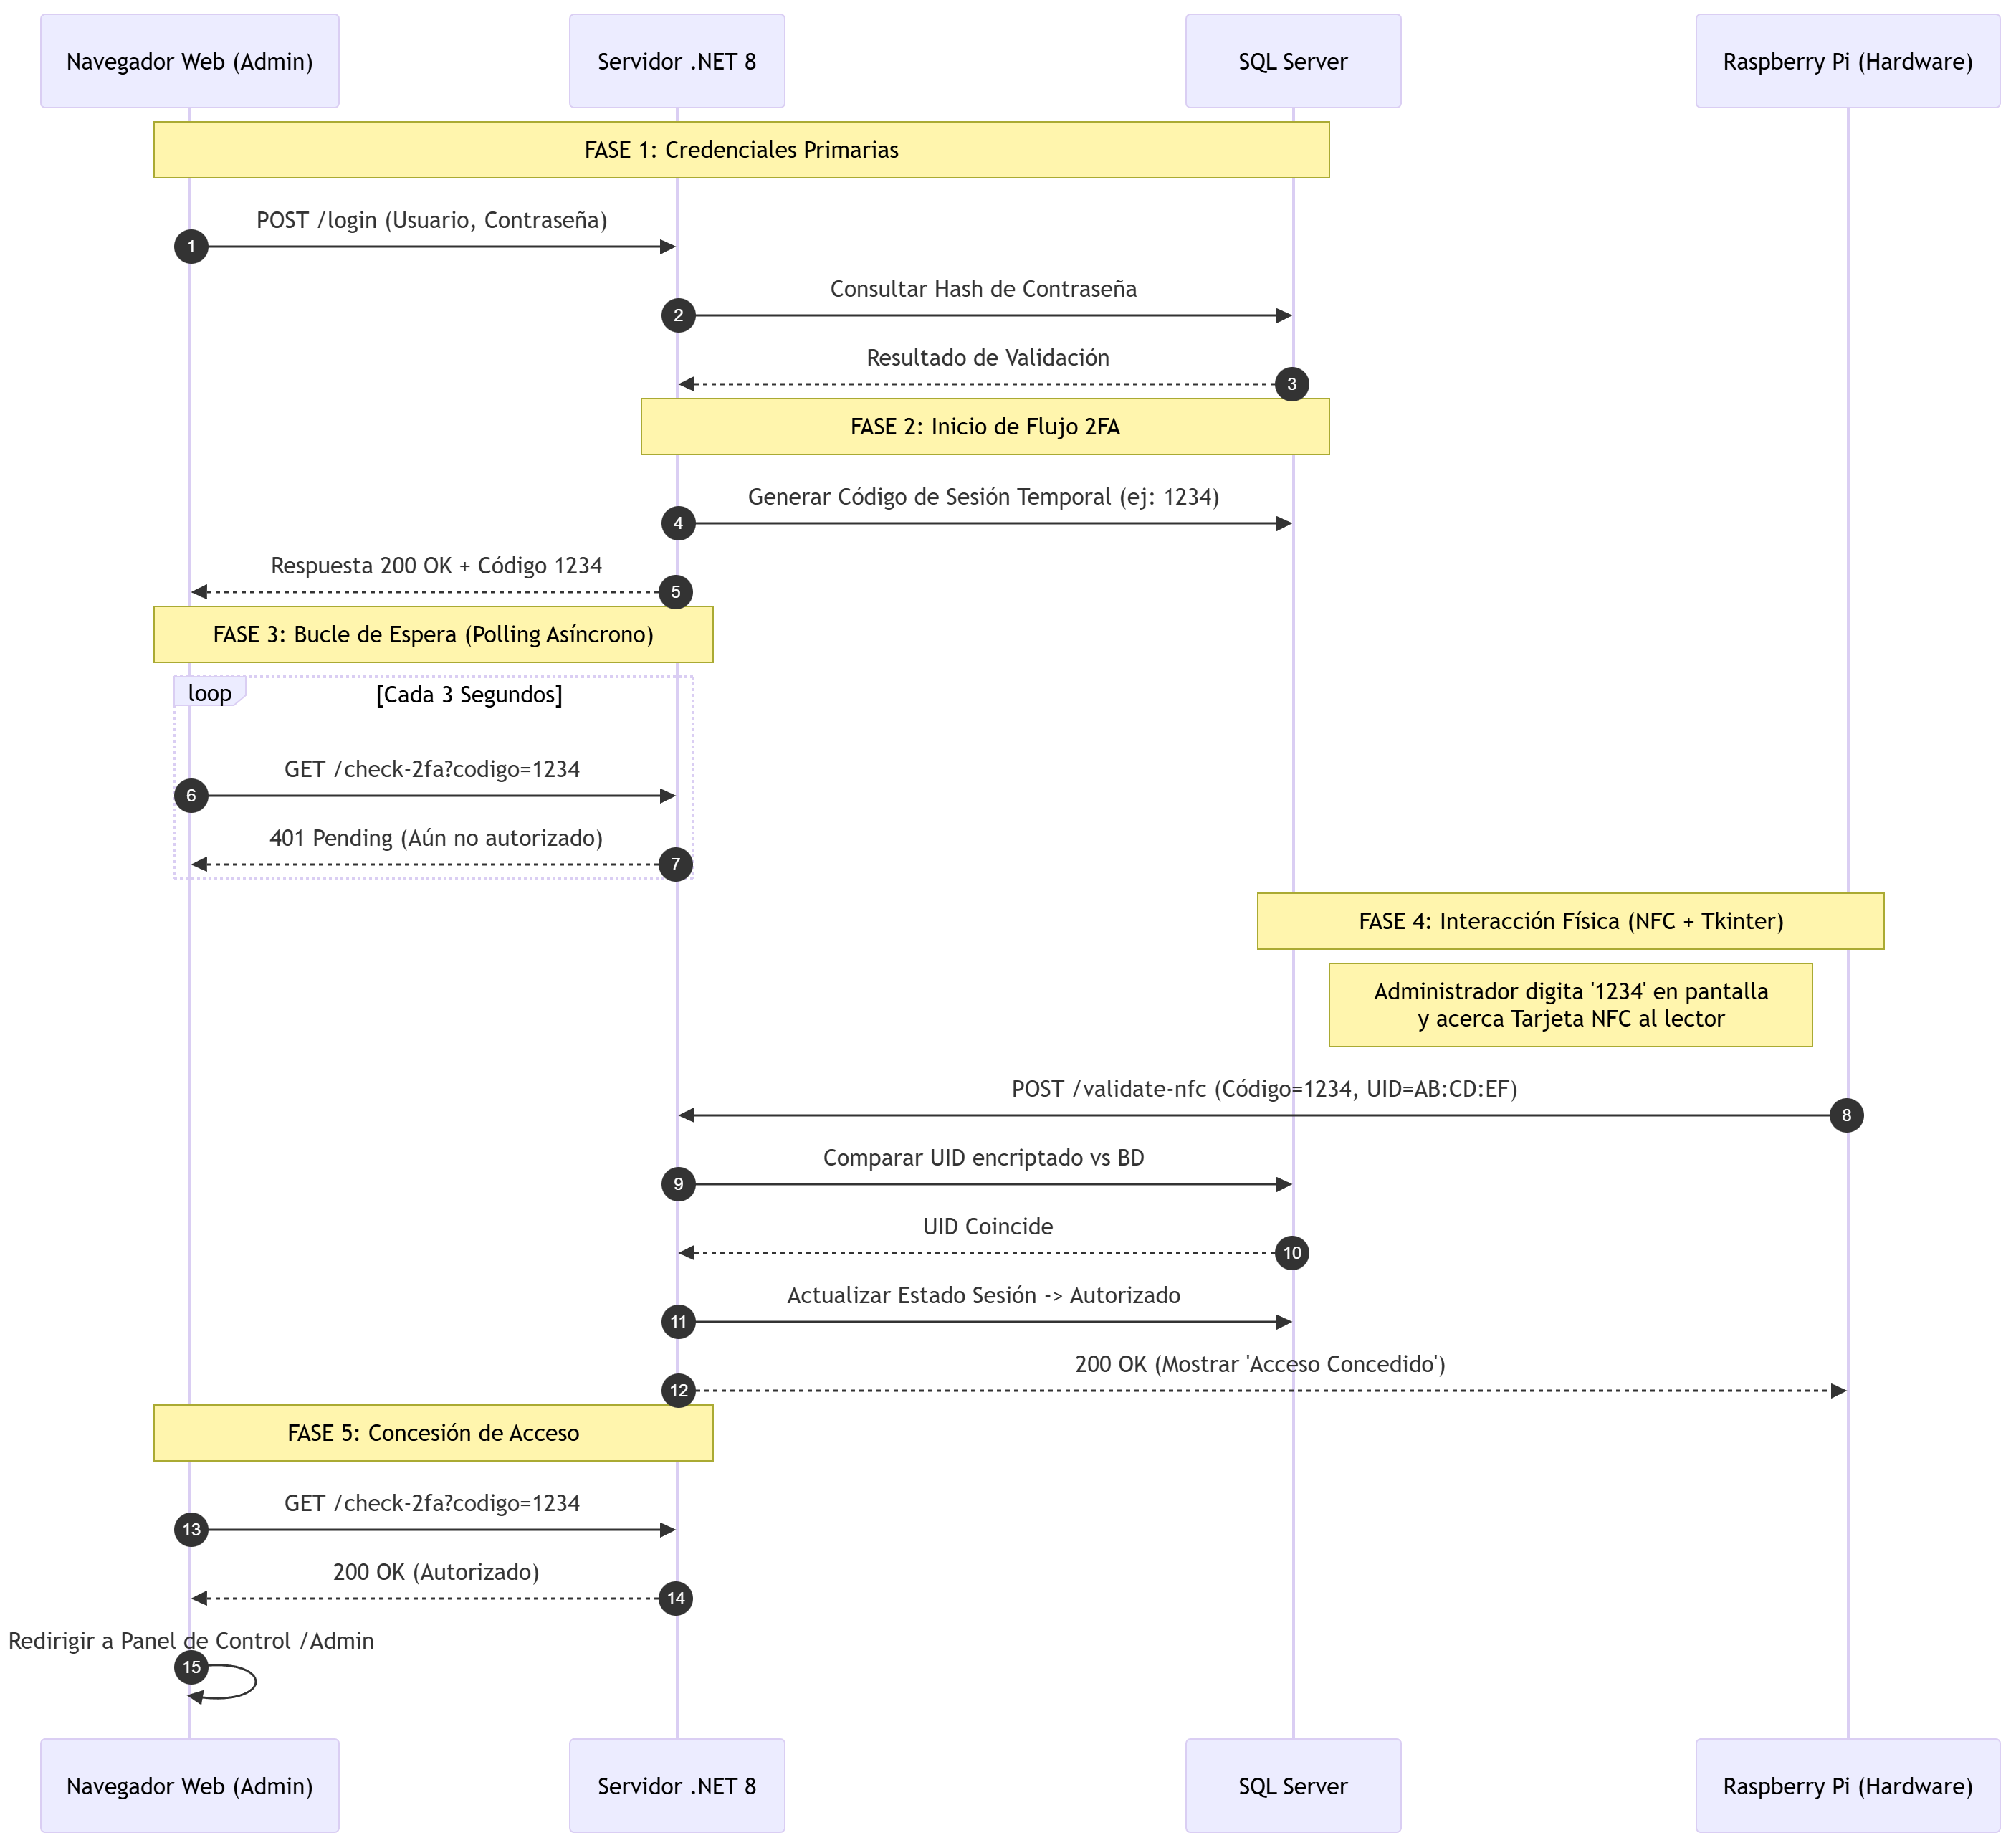
\includegraphics[width=0.98\textwidth]{imagenes/diagrama_secuencia_2fa.png} 
	\caption{Diagrama de Secuencia UML detallando el proceso de autenticación de doble factor y comunicación con la API (Creado en Mermaid.live).}
	\label{fig:uml_secuencia_2fa}
\end{figure}


\subsection{Diseño e Integración Física del Módulo (Impresión 3D)}

Para asegurar la durabilidad del módulo en entornos comerciales, se desarrolló una carcasa personalizada que integra la Raspberry Pi, la pantalla táctil y el lector NFC en una unidad compacta y ergonómica. El modelado 3D se basó en un levantamiento dimensional preciso de los componentes para garantizar un ensamblaje libre de tensiones mecánicas en los puertos y conexiones GPIO.

Una consideración técnica clave fue la ubicación del módulo RFID-RC522. El soporte interno fija el sensor de forma que su antena permanezca paralela a la cara interna del chasis. Dado que los polímeros de impresión no bloquean las señales de 13.56 MHz, la lectura de tarjetas es efectiva a través del material. Este diseño mantiene la electrónica sellada y protegida contra derrames de líquidos o suciedad, riesgos críticos en la operación de un restaurante.

La materialización se realizó mediante impresión 3D por deposición de hilo fundido (FDM). La Figura \ref{fig:carcasa} muestra el modelo digital diseñado y la Figura \ref{fig:carcasa_render} presenta el ensamblaje final, consolidando los componentes individuales en un dispositivo operativo tipo appliance.

% Opción A: Imágenes una debajo de la otra
\begin{figure}[H]
	\centering
	\includegraphics[width=0.8\textwidth]{imagenes/carcasa.png} 
	\caption{Modelado 3D de la carcasa protectora (Creado en Cinema 4D Trial Version)}
	\label{fig:carcasa}
\end{figure}

\begin{figure}[H]
	\centering
	\includegraphics[width=0.8\textwidth]{imagenes/carcasa_mult.png} 
	\caption{Modelado 3D de la carcasa protectora (Creado en Cinema 4D Trial Version)}
	\label{fig:carcasa_render}
\end{figure}

%%%%%%%%%%%

\section{Pruebas de Validación y Verificación}
En estricto cumplimiento con el diseño metodológico trazado en la fase de formulación del proyecto, la etapa de pruebas de validación y verificación se estructuró con el propósito de evaluar la funcionalidad, el rendimiento y la seguridad del sistema en un entorno que simulara fielmente las limitaciones tecnológicas reales de un restaurante PYME. 

Para abarcar integralmente el comportamiento del software, el plan de pruebas se dividió en cuatro frentes de evaluación: validación manual de usabilidad, pruebas unitarias de seguridad y lógica de negocio, pruebas automatizadas de estrés, y medición de latencia operativa.

\subsection{Infraestructura y Entorno de Laboratorio}
Para garantizar que el desempeño de la aplicación corresponda a la realidad económica de los establecimientos objetivo, la infraestructura del servidor principal —encargada de procesar la lógica de negocio en .NET 8 y gestionar la persistencia en la base de datos SQL Server— se desplegó de manera deliberada en un equipo con recursos heredados. Se utilizó un computador portátil DELL (año de fabricación 2008), equipado con un procesador Intel Core 2 Duo (T8000), 8 GB de memoria RAM DDR2 y un disco duro mecánico (HDD). Para maximizar la asignación de recursos hacia el sistema web, este equipo operó bajo el sistema operativo Windows 10 LTSC (Long-Term Servicing Channel).

La red de intranet fue gestionada mediante un router doméstico ZTE ZXV10 W300, operando estrictamente en modo local sin salida a internet. Para replicar la topología de red de un restaurante y evaluar el impacto de las conexiones mixtas, los clientes que simularon los módulos fijos (Cocina y Caja) fueron conectados mediante cableado a los puertos LAN. En contraste, el equipo encargado de simular al Mesero se enlazó exclusivamente a través de la interfaz inalámbrica en la banda Wi-Fi de 2.4 GHz. Esta distinción física resultó fundamental para introducir latencia real, susceptibilidad a interferencias y fluctuaciones de red, emulando el comportamiento de un dispositivo móvil operado en constante movimiento. Debido a requerimientos de compatibilidad del entorno de automatización, los clientes de prueba operaron bajo el sistema operativo Ubuntu.

\subsection{Verificación Manual de Funcionalidades}
Esta etapa consistió en una auditoría de completitud del software mediante pruebas manuales controladas. El propósito fue confirmar que la arquitectura final del sistema no omitiera ninguna de las herramientas operativas requeridas por los diferentes roles de usuario, garantizando la usabilidad de las interfaces gráficas.

Mediante una lista de verificación (\textit{Checklist}) trazada desde la matriz de requerimientos, se inspeccionaron los módulos de la plataforma:
\begin{itemize}
	\item \textbf{Módulo de Administrador:} Gestión de menú, reportes de ventas y administración de perfiles de empleados.
	\item \textbf{Módulo de Mesero:} Interfaz táctil para la toma ágil de pedidos, envío de comandas y visualización del estado de las mesas.
	\item \textbf{Módulo de Cocina:} Recepción en tiempo real de órdenes estructuradas y actualización del estado de preparación de los platos.
	\item \textbf{Módulo de Caja:} Acceso al resumen de cuentas por mesa, facturación y generación del cierre de servicio.
\end{itemize}

\subsection{Pruebas Unitarias y de Seguridad Lógica}
Para certificar la robustez interna de la aplicación, especialmente en el manejo de datos sensibles y control de accesos, se incorporó una batería de pruebas a nivel de código utilizando el marco de pruebas \textit{MSTest} para .NET 8. 

A diferencia de las pruebas de interfaz, estas evaluaciones se enfocaron en validar de forma aislada la lógica de negocio y los componentes de seguridad implementados en el \textit{backend}. Los escenarios evaluados incluyeron:
\begin{itemize}
	\item \textbf{Cifrado e Integridad:} Validación de los algoritmos de encriptación de credenciales en la base de datos, asegurando que no existan vulnerabilidades de almacenamiento en texto plano.
	\item \textbf{Control de Autorización:} Verificación de los filtros de sesión, garantizando que un usuario con un rol inferior (ej. Mesero) no pueda ejecutar métodos HTTP restringidos a roles superiores (ej. Administrador).
	\item \textbf{Autenticación de Doble Factor (2FA):} Pruebas de integración sobre los servicios que procesan los identificadores criptográficos generados por las tarjetas NFC, validando su correcta asociación con los usuarios registrados en SQL Server a través de Entity Framework 6.
\end{itemize}

\subsection{Pruebas Automatizadas de Concurrencia}
Para superar las limitaciones de una prueba manual esporádica y garantizar la estabilidad del sistema ante cargas de trabajo prolongadas, la validación operativa se llevó a cabo utilizando scripts automatizados desarrollados en \textit{Playwright} con Node.js. 

Se estructuró un entorno de estrés donde agentes virtuales autónomos interactuaron de manera simultánea durante una jornada operativa simulada de 9 horas ininterrumpidas. El agente \textit{Mesero} generó ráfagas constantes de pedidos, mientras que los agentes de \textit{Cocina} y \textit{Caja} interceptaron y despacharon estas solicitudes. Los resultados de esta ejecución masiva fueron recolectados en registros tabulares (archivos CSV) para documentar la tasa de éxito transaccional. Este enfoque validó la capacidad de Entity Framework 6 para procesar múltiples peticiones simultáneas sin generar interbloqueos (\textit{deadlocks}) ni corrupción de información referencial.

\subsection{Evaluación del Tiempo de Respuesta Operativa}
En estricta correspondencia con el objetivo de erradicar los retrasos del modelo manual de toma de pedidos, se ejecutó la medición empírica de la latencia del sistema. El registro de tiempos se focalizó en las operaciones transaccionales más demandantes utilizando herramientas de diagnóstico (\textit{DevTools - Network}) y cronometría física:
\begin{itemize}
	\item El tiempo neto desde que el Mesero confirma una comanda hasta que es persistida en la base de datos y renderizada en la pantalla de Cocina.
	\item La latencia en la resolución de consultas financieras y de inventario complejas.
	\item El tiempo de procesamiento del hardware 2FA, abarcando desde el contacto de la tarjeta física con el lector RFID-RC522 en la Raspberry Pi, hasta que el cliente Python valida el identificador con la API .NET y el sistema web autoriza el inicio de sesión.
\end{itemize}

El criterio de aceptación ineludible dicta que, incluso operando sobre el hardware heredado evaluado, el tiempo de respuesta total para cualquiera de estas operaciones críticas no debe exceder el umbral máximo de \textbf{2.0 segundos}.

\newpage
\chapter{RESULTADOS}
%%%%%%%%%%%%%%%%%%%%%%%%%%%%%%%%%%
\section{Resultados de la Verificación Manual de Funcionalidades}

Para garantizar el correcto funcionamiento del sistema y su alineación con los requerimientos establecidos en la fase de diseño, se ejecutó un proceso de validación operativa integral. Esta etapa consistió en un recorrido sistemático a través de las interfaces gráficas correspondientes a cada uno de los roles del restaurante, simulando escenarios reales de operación diaria. El objetivo principal fue comprobar la disponibilidad y estabilidad de las herramientas de gestión asignadas a los perfiles de administrador, mesero, cocina y caja, asegurando que el flujo de la información se mantuviera continuo desde la toma del pedido hasta su facturación final.

Durante las pruebas, se comprobó que el módulo del administrador permite la correcta creación y modificación del catálogo de productos, así como la gestión de usuarios del sistema. Por su parte, la interfaz destinada al personal de servicio demostró una adecuada respuesta táctil en dispositivos móviles, facilitando la selección ágil de los platos y el envío inmediato de la comanda hacia el área de preparación. En el módulo de cocina, se validó la actualización de los pedidos entrantes mediante la visualización horizontal planificada, lo cual permitió a los operarios modificar el estado de los alimentos a preparados de manera dinámica. Finalmente, en el perfil de caja, se verificó la recepción oportuna de las órdenes listas y la correcta liquidación de las mesas, confirmando la persistencia de los datos en el historial transaccional.

Los resultados de esta auditoría funcional evidenciaron el cumplimiento de los flujos operativos básicos planeados para la aplicación. A continuación, la Tabla \ref{tab:verificacion_manual} consolida los escenarios evaluados y el estado final de aprobación para cada rol operativo del sistema.

\begin{table}[H]
	\centering
	\caption{Resultados de la verificación manual de funcionalidades operativas por rol.}
	\label{tab:verificacion_manual}
	\small
	% Usamos tabularx para ajuste automático. 'l' para el rol, 'X' para la descripción (ajustable) y 'c' para el resultado.
	\begin{tabularx}{\textwidth}{l X c}
		\toprule
		\textbf{Rol Operativo} & \textbf{Funcionalidad Evaluada} & \textbf{Resultado} \\
		\midrule
		Administrador & Creación y edición de productos en el menú, visualización de inventario y registro de nuevos empleados. & Cumple \\
		\midrule
		Mesero & Ingreso al sistema, selección de mesa activa, registro de productos mediante interfaz táctil y envío de comanda. & Cumple \\
		\midrule
		Cocina & Recepción visual de la comanda en pantalla horizontal, identificación por colores y actualización de estado a listo. & Cumple \\
		\midrule
		Caja & Visualización de comandas terminadas, generación del total de la factura y cierre transaccional de la mesa. & Cumple \\
		\bottomrule
	\end{tabularx}
\end{table}

Como evidencia visual del flujo de comunicación descrito, se capturó de forma simultánea el momento clave de la interacción entre las áreas operativas. La Figura \ref{fig:flujo_mesero_cocina} expone en paralelo la vista del mesero al momento de crear una orden y el panel de control del área de preparación al recibirla. Esta representación conjunta evidencia la correcta adaptación de la interfaz móvil a pantallas reducidas para agilizar el registro por parte del personal de servicio, mientras ilustra la recepción inmediata de la comanda en la cocina, corroborando la sincronización del sistema y el contraste visual diseñado para facilitar la lectura a distancia.

\begin{figure}[htpb]
	\centering
	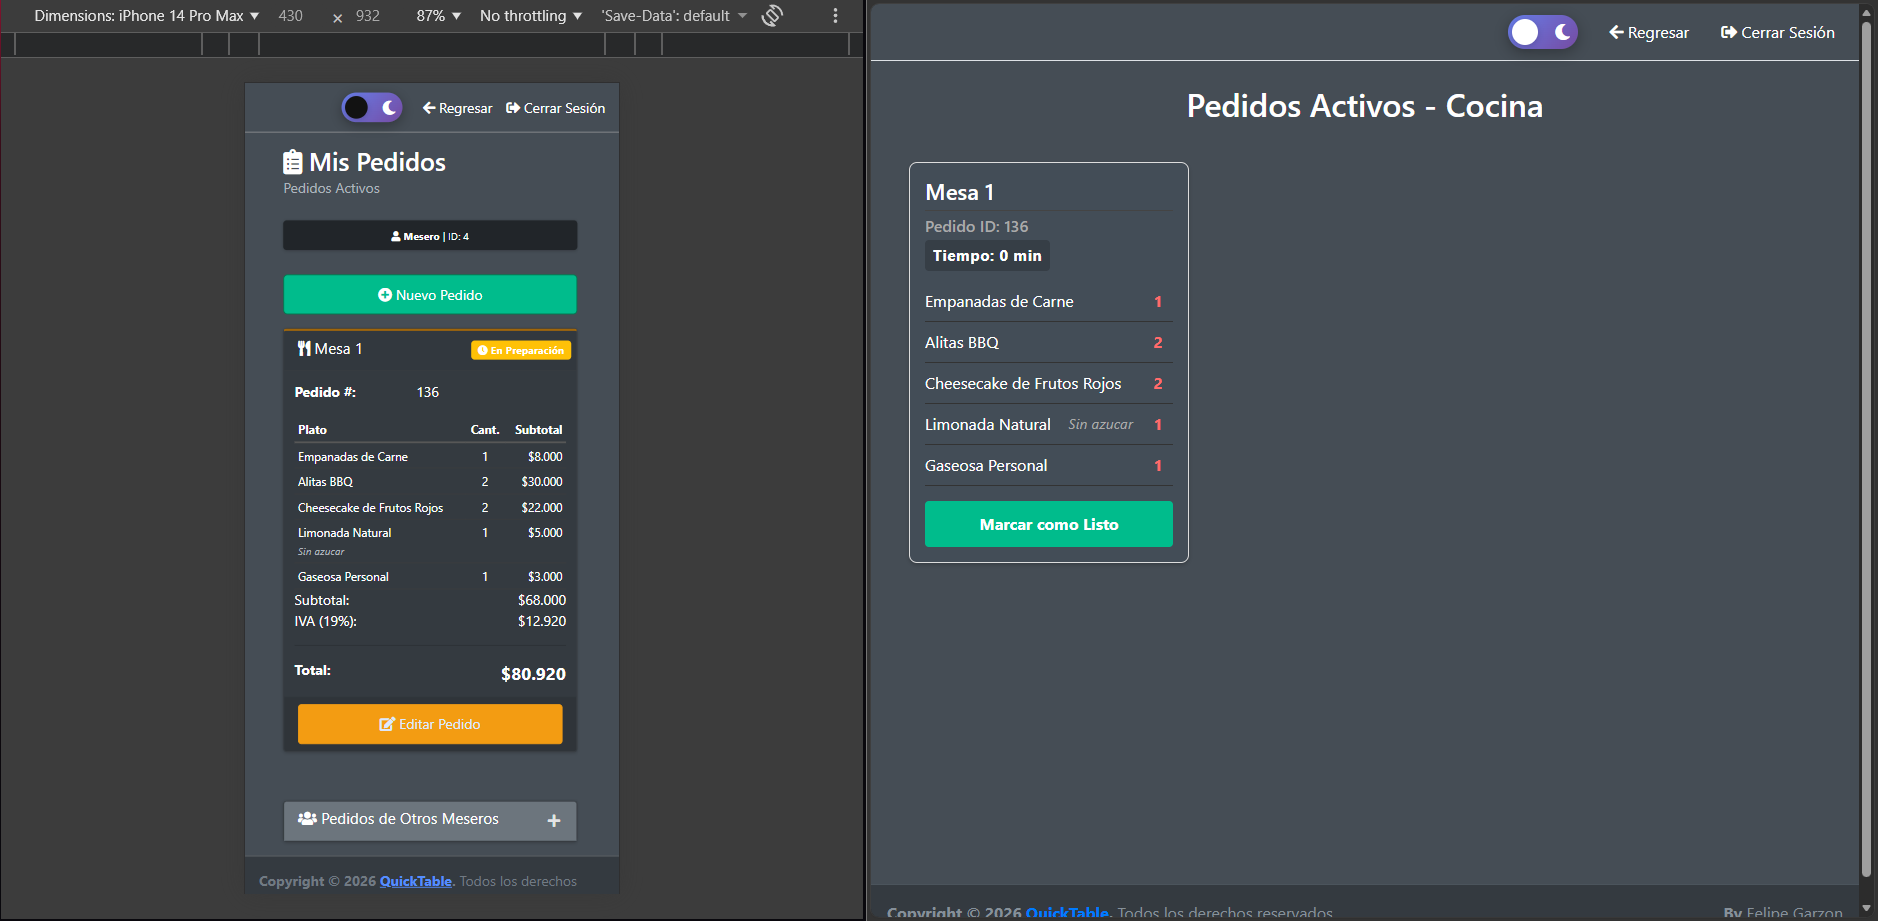
\includegraphics[width=0.95\textwidth]{Verificación Manual de Funcionalidades.png}
	\caption{Vista en paralelo de la interfaz de mesero durante la creación de la comanda y su recepción inmediata en el panel de control de cocina.}
	\label{fig:flujo_mesero_cocina}
\end{figure}
%%%%%%%%%%%%%%%%%%%%%%%%%%%

\section{ Resultados de las Pruebas Unitarias}

Las pruebas unitarias se ejecutaron sobre los servicios \texttt{PasswordService} y
\texttt{CryptoService}, los cuales concentran la lógica de protección de credenciales
y el cifrado de identificadores NFC en el sistema. Para \texttt{PasswordService}, los
casos de prueba cubrieron la generación del hash de contraseña mediante BCrypt con
factor de trabajo 12, la verificación de una contraseña válida contra su hash almacenado
y la verificación de una contraseña inválida, incluyendo el comportamiento del servicio
ante entradas vacías o nulas. Para \texttt{CryptoService}, los casos cubrieron el
cifrado de un UID de tarjeta mediante AES, la recuperación del valor original a través
del descifrado y la respuesta del servicio ante una cadena de entrada no válida.

\begin{table}[H]
	\centering
	\caption{Casos de prueba ejecutados con MSTest}
	\label{tab:mstest}
	\small
	\begin{tabular}{l l c}
		\toprule
		\textbf{Servicio} & \textbf{Caso de prueba} & \textbf{Resultado} \\
		\midrule
		PasswordService & HashPassword genera hash no vacío & Passed \\
		PasswordService & VerifyPassword con contraseña válida & Passed \\
		PasswordService & VerifyPassword con contraseña inválida & Passed \\
		\midrule
		CryptoService & EncriptarUID produce cadena cifrada & Passed \\
		CryptoService & DesencriptarUID recupera el valor original & Passed \\
		\bottomrule
	\end{tabular}
\end{table}

La Figura \ref{fig:mstest1} presenta la primera ejecución del conjunto de pruebas,
donde se registró la resolución de cada caso junto con el tiempo de ejecución por
prueba. La Figura \ref{fig:mstest2} corresponde a la segunda ejecución del mismo
conjunto, realizada para verificar la repetibilidad de los resultados.

\begin{figure}[H]
	\centering
	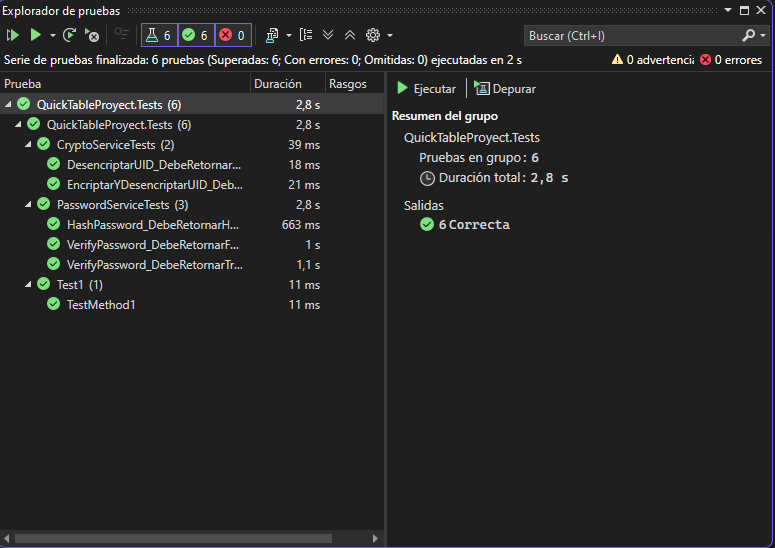
\includegraphics[width=0.85\textwidth]{ResultadoMSTest.png}
	\caption{Primera ejecución del conjunto de pruebas unitarias MSTest}
	\label{fig:mstest1}
\end{figure}

\begin{figure}[H]
	\centering
	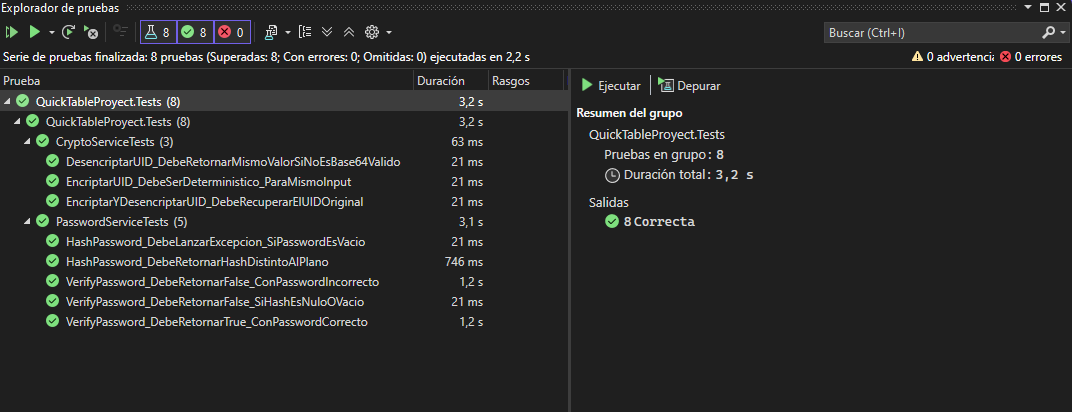
\includegraphics[width=0.85\textwidth]{ResultadoMSTestV2.png}
	\caption{Segunda ejecución del conjunto de pruebas unitarias MSTest}
	\label{fig:mstest2}
\end{figure}

En ambas ejecuciones, los 7 casos registraron estado \texttt{Passed}. El comportamiento
de \texttt{VerifyPassword} ante entradas vacías retorna \texttt{false} sin lanzar
excepción, resultado del bloque de validación previo al llamado de BCrypt. De igual
forma, \texttt{DesencriptarUID} retorna el valor de entrada sin modificación cuando la
cadena recibida no corresponde a un Base64 válido, comportamiento definido por el bloque
\texttt{catch} del método, el cual devuelve el parámetro \texttt{uidEncriptado}
directamente.


%%%%%%%%%%%%%%%%%%%%%%%%%%%%%%%
\section{Resultados de las Pruebas de API con Postman}

Con el fin de complementar la validación funcional del sistema, se realizaron pruebas directas sobre los puntos de acceso HTTP expuestos por el backend, empleando la herramienta Postman como cliente de solicitudes. Esta fase permitió verificar de forma aislada la coherencia semántica de las respuestas JSON retornadas por los controladores, sin intermediación de la interfaz gráfica, cubriendo los servicios de gestión de copias de seguridad y control de asistencia del personal.


\subsection{Creación de Copia de Seguridad}

La solicitud dirigida al endpoint de creación de respaldos generó una respuesta satisfactoria 
del servidor. El controlador procesó la petición, ejecutó el procedimiento de volcado de la 
base de datos sobre el almacenamiento local del servidor y retornó un objeto JSON con los 
metadatos técnicos del archivo generado, confirmando la integridad de la operación.


\begin{table}[H]
	\centering
	\caption{Metadatos retornados por el endpoint de creación de respaldo.}
	\label{tab:postman_crear_backup}
	\small
	% Usamos tabular con un ancho de columna manual para la derecha
	\begin{tabular}{l p{7cm}}
		\toprule
		\textbf{Campo} & \textbf{Valor obtenido} \\ 
		\midrule
		\texttt{success}       & \texttt{true} \\
		\texttt{message}       & Backup creado exitosamente \\
		\texttt{nombreArchivo} & \texttt{QuickTableDB\_20260413\_103531.bak} \\
		\texttt{tamanioMB}     & 6,12 MB \\
		\texttt{backupId}      & 1001 \\
		\bottomrule
	\end{tabular}
\end{table}


\begin{figure}[H]
	\centering
	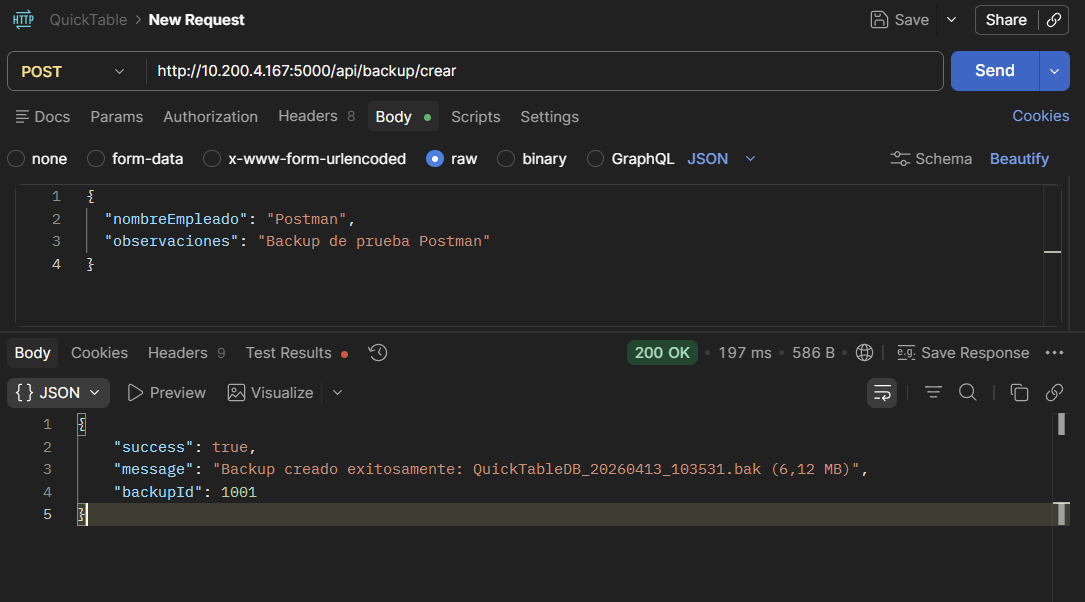
\includegraphics[width=0.8\textwidth]{CrearBackup.png}
	\caption{Respuesta del servidor ante la solicitud de creación de archivo de respaldo, 
		visualizada en Postman.}
	\label{fig:postman_crear_backup}
\end{figure}

\subsection{Consulta de Espacio de Almacenamiento Disponible}

Se ejecutó una petición \texttt{GET} para determinar la capacidad de almacenamiento libre 
en el servidor anfitrión. La API retornó un único campo numérico entero expresado en 
megabytes (MB), confirmando la disponibilidad del servicio de monitoreo del sistema de 
archivos. El valor obtenido, \texttt{28444 MB} equivalentes a aproximadamente 24 GB, 
verifica que el servidor dispone de capacidad suficiente para operaciones continuadas de 
respaldo durante el ciclo de vida del sistema.

\begin{figure}[H]
	\centering
	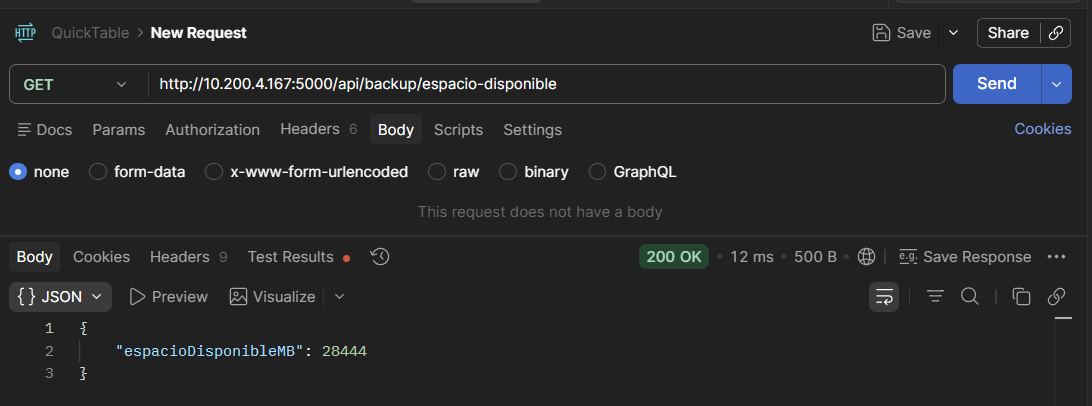
\includegraphics[width=0.8\textwidth]{Espacio Disponible.png}
	\caption{Métrica de almacenamiento disponible retornada por el endpoint.}
	\label{fig:postman_espacio}
\end{figure}

\subsection{Listado del Historial de Respaldos}

Se validó la recuperación del registro histórico de copias de seguridad almacenadas en el 
sistema. La respuesta consistió en un arreglo de objetos JSON donde cada elemento describe 
un respaldo individual con sus atributos operativos y de seguridad. El análisis de la 
respuesta permitió verificar los siguientes aspectos del sistema de persistencia:

\begin{enumerate}
	\item \textbf{Trazabilidad operativa:} Cada registro incluye la marca temporal de 
	creación, el nombre del archivo \texttt{.bak}, su ruta física en el servidor y el 
	usuario creador, permitiendo auditar el historial de operaciones de mantenimiento.
	\item \textbf{Seguridad criptográfica:} La respuesta expone las rutas de los 
	certificados de cifrado (\texttt{.cer}) y las claves privadas (\texttt{.pvk}) 
	asociadas a cada respaldo, evidenciando la integración del módulo de 
	Cifrado Transparente de Datos (TDE) con el proceso de respaldo.
	\item \textbf{Consistencia de registros:} Los tres respaldos listados presentaron 
	estado \texttt{Exitoso} y un tamaño consistente entre 5{,}18 MB y 5{,}24 MB, 
	lo que confirma la estabilidad del procedimiento de volcado entre sesiones 
	de ejecución independientes.
\end{enumerate}

\begin{figure}[H]
	\centering
	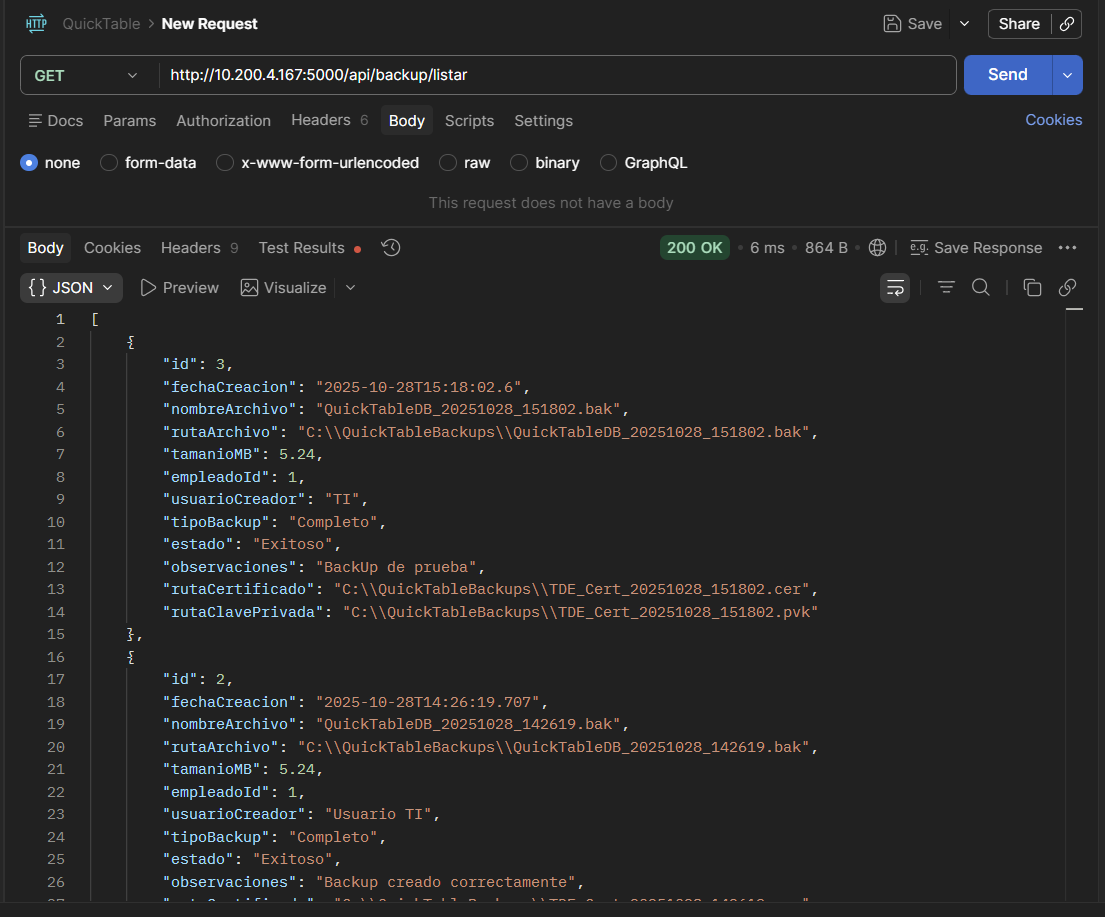
\includegraphics[width=0.8\textwidth]{Backup listar.png}
	\caption{Arreglo JSON retornado por el endpoint de listado, evidenciando el historial 
		de respaldos con sus metadatos de seguridad asociados.}
	\label{fig:postman_listar_backup}
\end{figure}

\subsection{Registro de Salida de Personal mediante Tarjeta NFC}

Se evaluó el endpoint de cierre de jornada laboral, el cual forma parte del subsistema de 
control de asistencia integrado con el módulo de hardware NFC. Para esta prueba, el 
identificador único (UID) de la tarjeta del empleado fue codificado en Base64 y transmitido 
al servidor mediante una solicitud \texttt{POST}, replicando el comportamiento del cliente 
Python ejecutado en la Raspberry Pi. El sistema localizó el registro de sesión activo 
correspondiente al día en curso, ejecutó el cálculo automático del tiempo laborado a partir 
de la marca temporal de ingreso previamente almacenada y retornó la confirmación estructurada 
de la operación, como se detalla en la Tabla~\ref{tab:postman_salida}.

\begin{table}[H]
	\centering
	\caption{Campos retornados por el endpoint de registro de salida de personal.}
	\label{tab:postman_salida}
	\small
	% Definimos dos columnas fijas para que no se estiren al infinito
	\begin{tabular}{l p{8cm}}
		\toprule
		\textbf{Campo} & \textbf{Valor registrado} \\ 
		\midrule
		\texttt{success}         & \texttt{true} \\
		\texttt{message}         & Salida registrada correctamente \\
		\texttt{nombre}          & cocina \\
		\texttt{rol}             & Cocina \\
		\texttt{horaIngreso}     & 08:23 \\
		\texttt{horaSalida}      & 10:03 \\
		\texttt{tiempoTrabajado} & 1h 40m \\
		\bottomrule
	\end{tabular}
\end{table}


\begin{figure}[H]
	\centering
	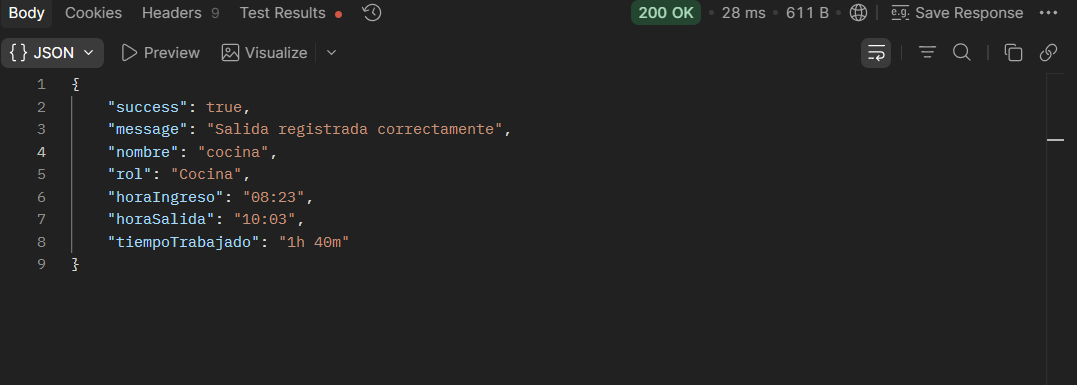
\includegraphics[width=0.8\textwidth]{Marcar SAlida.png}
	\caption{Respuesta del endpoint \texttt{/api/asistencia/marcar-salida} tras el cierre 
		exitoso de la jornada laboral del personal de cocina.}
	\label{fig:postman_salida}
\end{figure}



%%%%%%%%%%%%%%%%%%%%%%%%%%%%%%%%



\section{Resultados de la Evaluación del Tiempo de Respuesta Operativa}
Para esta fase se definieron dos condiciones de evaluación sobre el mismo aplicativo: una con acceso a internet y otra sin acceso a internet. 
En este apartado se presentan los resultados correspondientes a la condición con acceso a internet, dejando constancia de que existe una medición equivalente para la condición sin conectividad externa. 

\subsubsection{Condición con acceso a Internet}

La medición con acceso a internet se realizó sobre las vistas de Login, Mesero, Cocina, Caja y Administrador, empleando herramientas del navegador y reportes Lighthouse exportados en formato HTML.
Las variables registradas incluyen número de peticiones, peso transferido, tiempo hasta el primer byte, eventos de carga del documento y métricas visuales de Lighthouse.

\begin{table}[H]
	\centering
	\caption{Métricas registradas en la condición con acceso a internet.}
	\label{tab:devtools_con_internet}
	\small
	\begin{tabularx}{\textwidth}{l *{9}{>{\centering\arraybackslash}X}}
		\toprule
		\textbf{Vista} & \textbf{Pet.} & \textbf{Peso} & \textbf{TTFB} & \textbf{DCL} & \textbf{Load} & \textbf{FCP} & \textbf{LCP} & \textbf{CLS} & \textbf{Score} \\
		\midrule
		Login   & 14 & 12.1k & 9ms  & 214ms & 219ms & 0.7s  & 0.8s  & 0.06  & 99 \\
		Mesero  & 15 & 11.0k & 11ms & 212ms & 216ms & 3.2s  & 3.3s  & 0.016 & 86 \\
		Cocina  & 30 & 27.2k & 177ms& 563ms & 573ms & 0.6s  & 0.6s  & 0.087 & 98 \\
		Caja    & 21 & 19.8k & 14ms & 382ms & 389ms & 0.6s  & 0.7s  & 0.178 & 92 \\
		Admin   & 14 & 9.9k  & 9.9ms& 240ms & 245ms & 0.58s & 0.62s & 0     & 100 \\
		\bottomrule
	\end{tabularx}
	\begin{flushleft}
		\footnotesize
		\textbf{Pet.}: Peticiones; \textbf{DCL}: DOMContentLoaded; \textbf{FCP}: First Contentful Paint; \textbf{LCP}: Largest Contentful Paint; \textbf{CLS}: Cumulative Layout Shift.
	\end{flushleft}
\end{table}


La Tabla \ref{tab:devtools_con_internet} muestra que la vista de Login registró 14 peticiones, 12.1 kB transferidos y un evento \textit{Load} de 219 ms. 
La vista de Mesero registró 15 peticiones, 11.0 kB transferidos y un evento \textit{Load} de 216 ms. 
La vista de Cocina concentró el mayor número de solicitudes dentro de esta condición, con 30 peticiones y 27.2 kB transferidos.
Caja registró 21 peticiones y 19.8 kB transferidos, mientras que la vista de Administrador presentó 14 peticiones y 9.92 kB transferidos. 

El \textit{Time to First Byte} (TTFB), o tiempo hasta el primer byte, presentó diferencias entre las vistas evaluadas. 
Login, Mesero, Caja y Administrador registraron valores de 9 ms, 11 ms, 14 ms y 9.92 ms, respectivamente.
La vista de Cocina registró un TTFB de 177 ms, valor superior al resto de módulos analizados en esta condición.

En las métricas visuales, el \textit{First Contentful Paint} (FCP), o tiempo hasta la primera aparición visual de contenido, y el \textit{Largest Contentful Paint} (LCP), o tiempo hasta que se renderiza el elemento de mayor tamaño visible, se mantuvieron por debajo de un segundo en Login, Cocina, Caja y Administrador. 
Login presentó un FCP de 0.7 s y un LCP de 0.8 s. 
Cocina registró 0.6 s tanto en FCP como en LCP, mientras que Caja presentó 0.6 s y 0.7 s, respectivamente.
Administrador registró 0.582 s para FCP y 0.622 s para LCP.

La excepción en este conjunto fue la vista de Mesero, donde el FCP fue de 3.2 s y el LCP de 3.3 s. 
En este caso, la auditoría se ejecutó con \textit{form factor} móvil, perfil \textit{Slow 4G throttling}, latencia simulada de 150 ms, \textit{CPU slowdown multiplier} de 4 y agente emulado \textit{Moto G Power}. 
Estas condiciones se aplicaron para simular el uso del sistema desde un teléfono inteligente y no desde un equipo de escritorio. 

\begin{figure}[H]
	\centering
	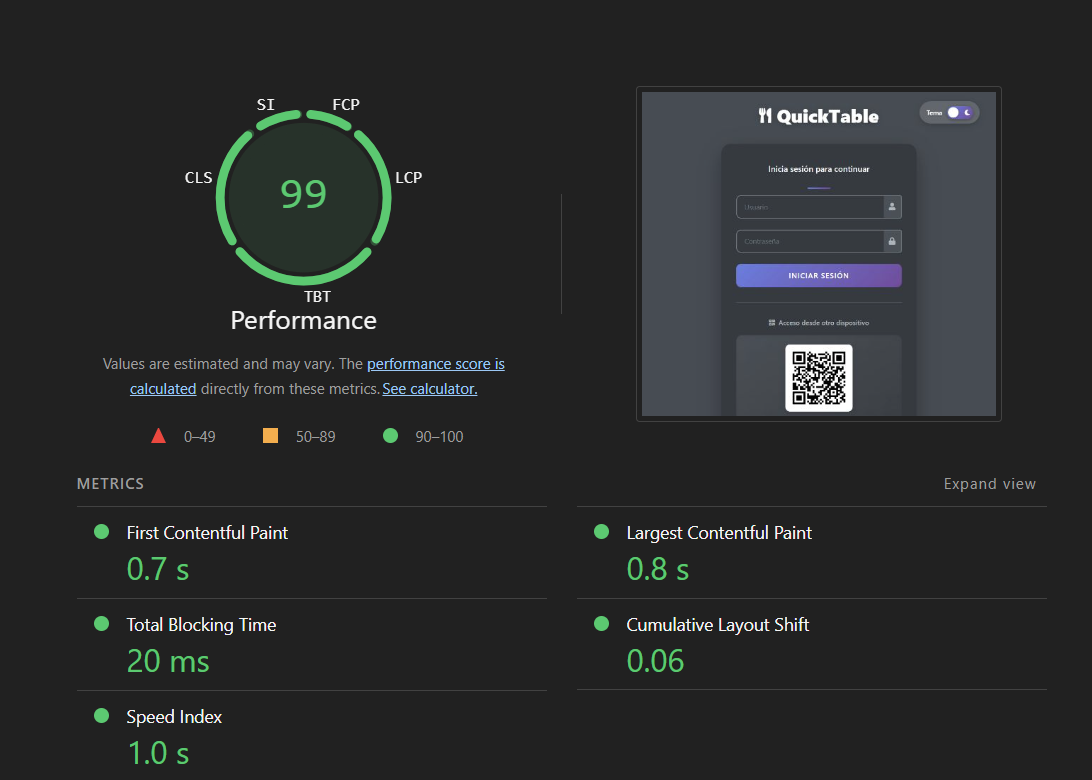
\includegraphics[width=0.8\textwidth]{login_lighthouse_resultado.png}
	\caption{Pantallazo del resultado Lighthouse para la vista de Login.}
	\label{fig:login_lighthouse_resultado}
\end{figure}

La evidencia visual de Login debe corresponder al pantallazo del resultado general del reporte HTML de Lighthouse, donde se observe el puntaje global y las métricas principales de la auditoría. 
Esta figura permite relacionar los valores reportados para FCP, LCP y estabilidad visual con la evidencia exportada por la herramienta. 

En las vistas de Cocina y Caja se identificó una diferencia entre el tiempo de carga inicial y la duración total observada en la actividad de red. 
En Cocina, la cadena de dependencias de red incluye solicitudes periódicas hacia el recurso \texttt{CocinaObtenerPedidosCocina}, lo que extiende la actividad observada más allá de la carga inicial de la interfaz.
En Caja ocurre un comportamiento equivalente con solicitudes hacia \texttt{CajaObtenerPedidosActivos}. 
Por esta razón, para interpretar la carga inicial de estas vistas resulta más representativo emplear los eventos \textit{Load} de 573 ms en Cocina y 389 ms en Caja. 

\begin{figure}[H]
	\centering
	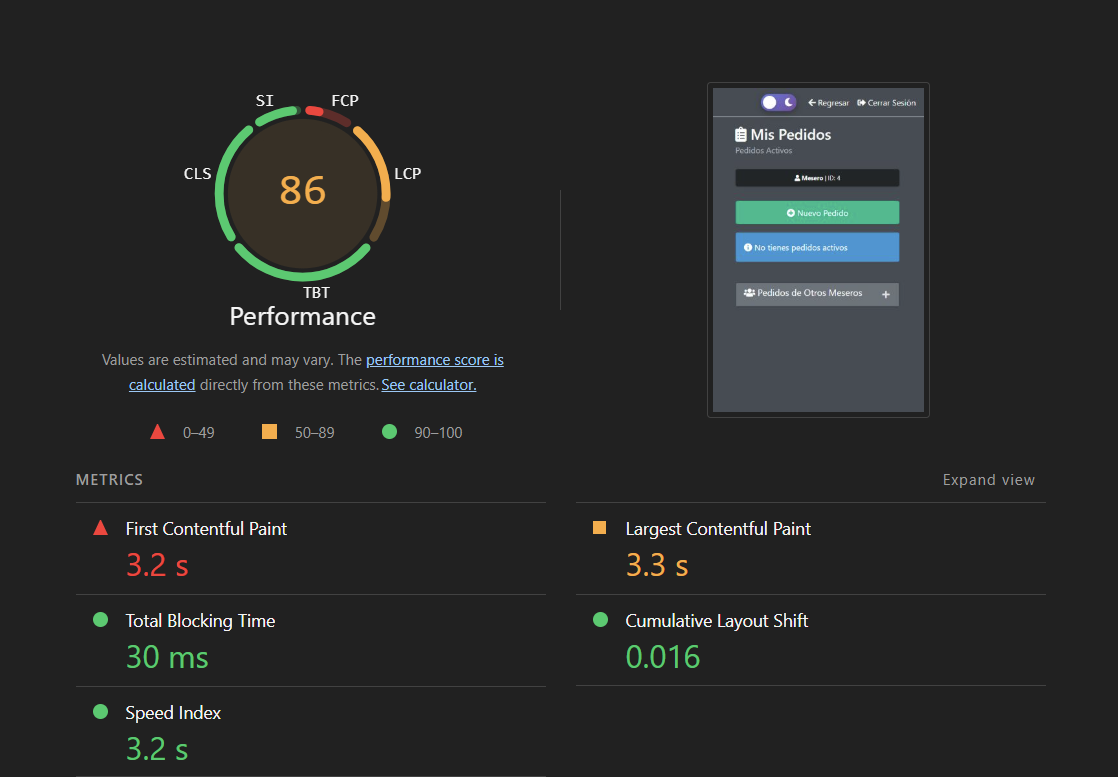
\includegraphics[width=0.8\textwidth, height=8.7cm]{mesero_lighthouse_resultado.png}
	\caption{Pantallazo del resultado Lighthouse para la vista de Mesero.}
	\label{fig:mesero_lighthouse_resultado}
\end{figure}

La evidencia visual de Mesero debe mostrar el resumen del reporte HTML de Lighthouse, junto con el contexto de auditoría móvil aplicado en la prueba. 
En este caso es pertinente que el pantallazo permita observar que la auditoría fue ejecutada para entorno móvil y con restricciones simuladas de red y procesamiento. 

\begin{figure}[H]
	\centering
	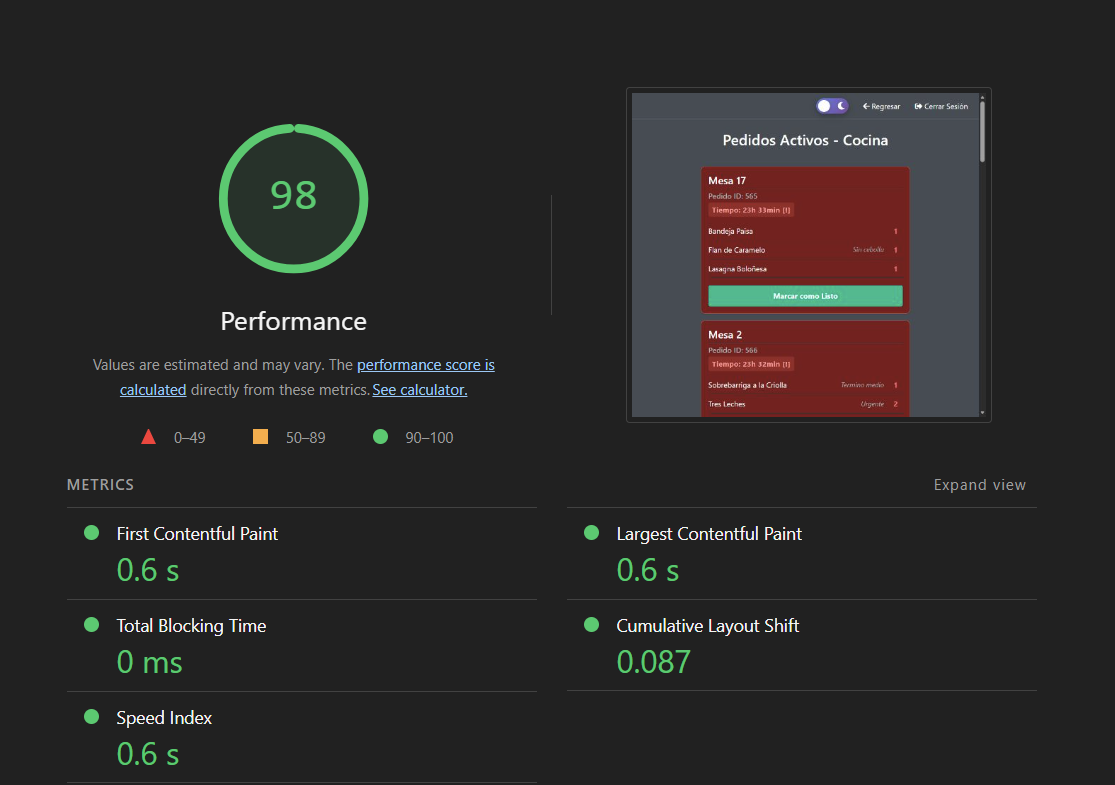
\includegraphics[width=0.8\textwidth, height=8.7cm]{cocina_lighthouse_resultado.png}
	\caption{Pantallazo del resultado Lighthouse para la vista de Cocina.}
	\label{fig:cocina_lighthouse_resultado}
\end{figure}

En Cocina, el reporte HTML también evidencia la presencia de solicitudes recurrentes en la red, asociadas a la consulta continua de pedidos activos.
Por ello, el pantallazo más útil para esta vista es el del resultado general de Lighthouse o, de forma complementaria, la sección de cadena de dependencias de red.

El \textit{Cumulative Layout Shift} (CLS), o desplazamiento acumulado del diseño, presentó su valor más alto en la vista de Caja con 0.178.
En el mismo reporte se identificó que el principal desplazamiento estuvo asociado al \textit{footer}, a la barra de navegación y a la carga de la fuente \texttt{fa-solid-900.woff2}.
En Login el CLS fue de 0.06, en Mesero de 0.016, en Cocina de 0.087 y en Administrador de 0.

\begin{figure}[H]
	\centering
	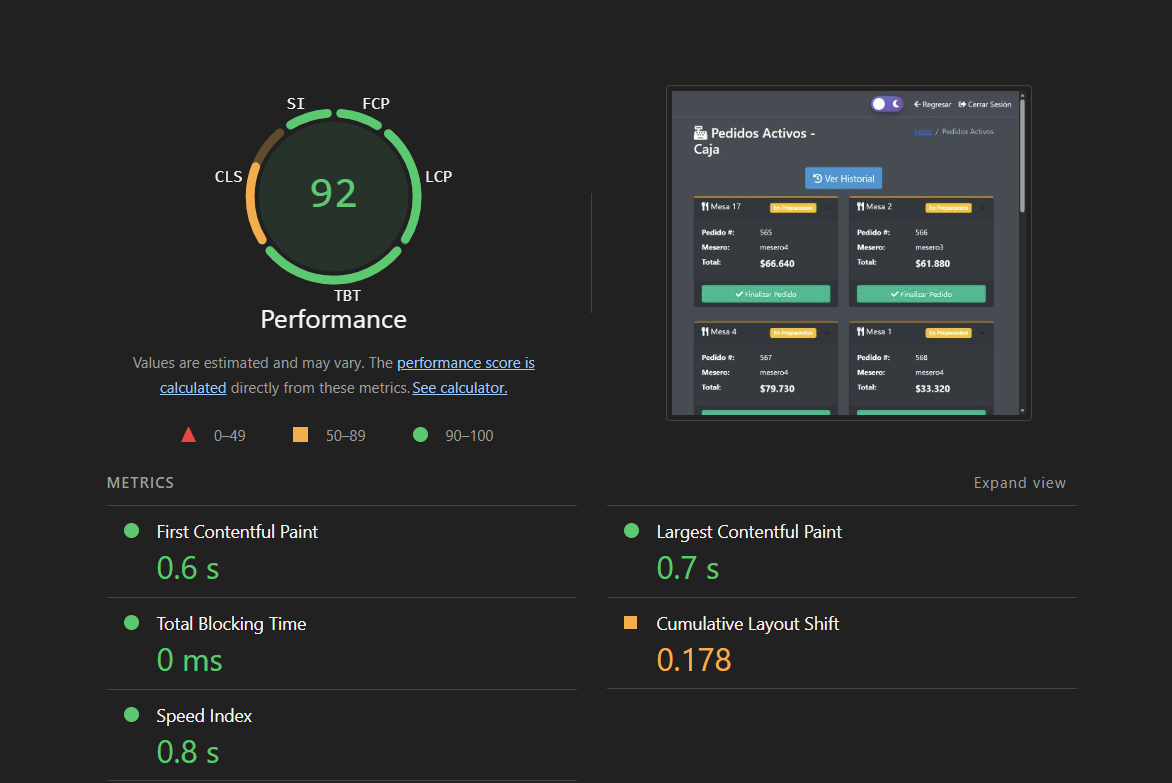
\includegraphics[width=0.8\textwidth]{caja_lighthouse_resultado.png}
	\caption{Pantallazo del resultado Lighthouse para la vista de Caja.}
	\label{fig:caja_lighthouse_resultado}
\end{figure}

En la vista de Caja resulta especialmente útil incluir un pantallazo del apartado de \textit{Layout shift culprits}, ya que allí se identifica el origen principal del desplazamiento visual observado durante la carga.
Esta evidencia complementa el valor de CLS reportado en la tabla y permite asociarlo con elementos concretos de la interfaz.

\begin{figure}[H]
	\centering
	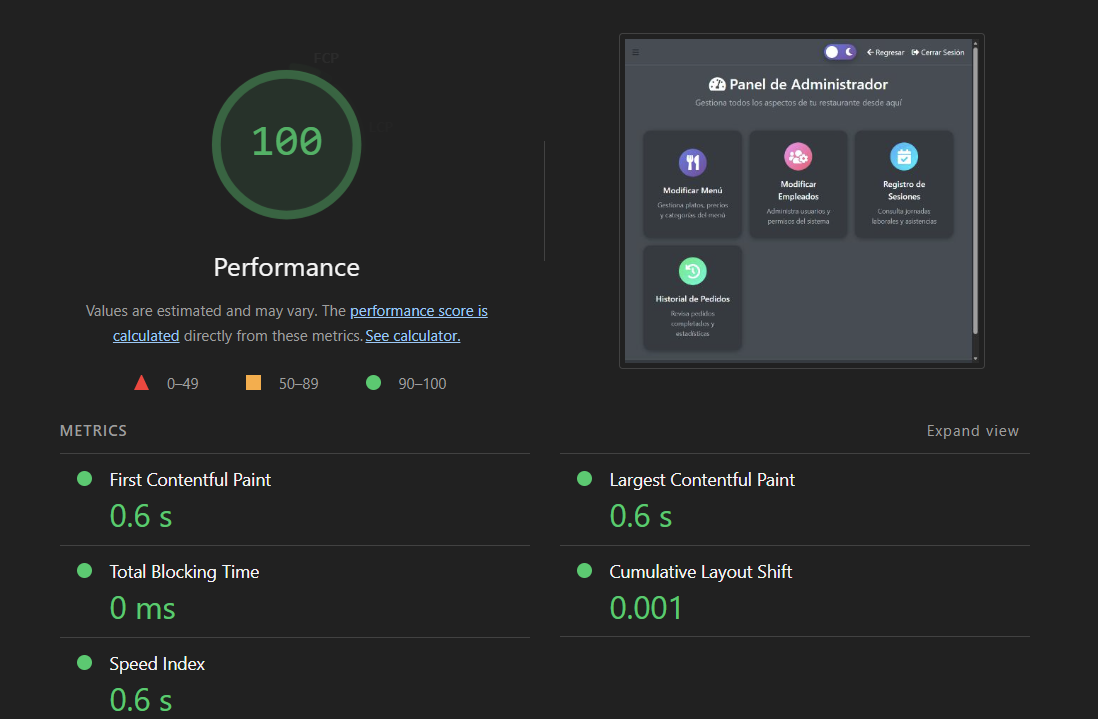
\includegraphics[width=0.8\textwidth,height=8cm]{admin_lighthouse_resultado.png}
	\caption{Pantallazo del resultado Lighthouse para la vista de Administrador.}
	\label{fig:admin_lighthouse_resultado}
\end{figure}

La vista de Administrador obtuvo un puntaje de 100, con FCP de 0.582 s, LCP de 0.622 s y CLS igual a 0. 
Por ello, el pantallazo del resultado general de Lighthouse es suficiente como evidencia principal para esta vista. 

%En conjunto, los reportes HTML de Lighthouse permiten documentar de forma homogénea los resultados obtenidos en cada módulo, ya que conservan tanto las métricas cuantitativas como las observaciones técnicas de cada auditoría.


\subsubsection{Condición sin acceso a Internet}

La medición sin acceso a internet se realizó sobre las mismas vistas, empleando herramientas del navegador y reportes Lighthouse exportados en formato HTML. 
Las variables registradas incluyen número de peticiones, peso transferido, tiempo hasta el primer byte, eventos de carga del documento y métricas visuales de Lighthouse. 

\begin{table}[H]
	\centering
	\caption{Métricas registradas en la condición sin acceso a internet.}
	\label{tab:devtools_sin_internet}
	\small
	\setlength{\tabcolsep}{2pt} % Ajuste fino para evitar desbordamiento
	% Definimos que todas las columnas numéricas sean X y centradas
	\begin{tabularx}{\textwidth}{l *{9}{>{\centering\arraybackslash}X}}
		\toprule
		\textbf{Vista} & \textbf{Pet.} & \textbf{Peso} & \textbf{TTFB} & \textbf{DCL} & \textbf{Load} & \textbf{FCP} & \textbf{LCP} & \textbf{CLS} & \textbf{Score} \\
		\midrule
		Login   & 15 & 477.1k & 13.9ms & 583ms & 587ms & 0.62s & 0.71s & 0     & 99 \\
		Mesero  & 16 & 12.9k  & 14.1ms & 104ms & 230ms & 1.79s & 1.87s & 0.007 & 87 \\
		Cocina  & 44 & 43.5k  & 8.3ms  & 306ms & 315ms & 0.58s & 0.66s & 0.006 & 99 \\
		Caja    & 14 & 9.2k   & 8.6ms  & 228ms & 236ms & 0.46s & 0.58s & 0     & 100 \\
		Admin   & 14 & 9.2k   & 9.9ms  & 240ms & 245ms & 0.58s & 0.62s & 0     & 99 \\
		\bottomrule
	\end{tabularx}
	\begin{flushleft}
		\footnotesize
		\textbf{Pet.}: Peticiones; \textbf{DCL}: DOMContentLoaded; \textbf{FCP}: First Contentful Paint; \textbf{LCP}: Largest Contentful Paint; \textbf{CLS}: Cumulative Layout Shift.
	\end{flushleft}
\end{table}

La Tabla \ref{tab:devtools_sin_internet} muestra que la vista de Login registró 15 peticiones, 477.12 KB transferidos y un evento \textit{Load} de 587 ms. 
La vista de Mesero registró 16 peticiones, 12.96 KB transferidos y un evento \textit{Load} de 230 ms. 
La vista de Cocina concentró el mayor número de solicitudes en esta condición, con 44 peticiones y 43.51 KB transferidos. 
Caja y la vista de Administrador registraron 14 peticiones cada una, con 9.29 KB transferidos en ambos casos. 

El \textit{Time to First Byte} (TTFB), o tiempo hasta el primer byte, se mantuvo bajo en todas las vistas evaluadas. 
Login, Mesero, Cocina, Caja y Administrador registraron valores de 13.97 ms, 14.19 ms, 8.31 ms, 8.61 ms y 9.92 ms, respectivamente. 

En las métricas visuales, el \textit{First Contentful Paint} (FCP), o tiempo hasta la primera aparición visual de contenido, y el \textit{Largest Contentful Paint} (LCP), o tiempo hasta que se renderiza el elemento de mayor tamaño visible, se mantuvieron por debajo de un segundo en Login, Cocina, Caja y Administrador. 
Login presentó un FCP de 0.620 s y un LCP de 0.710 s. 
Cocina registró 0.586 s y 0.666 s, mientras que Caja presentó 0.468 s y 0.588 s, respectivamente. 
Administrador registró 0.582 s para FCP y 0.622 s para LCP. 

La excepción en este conjunto fue la vista de Mesero, donde el FCP fue de 1.795 s y el LCP de 1.871 s. 
Aun así, el puntaje Lighthouse se mantuvo en 87 y el evento \textit{Load} fue de 230 ms. 

\begin{figure}[H]
	\centering
	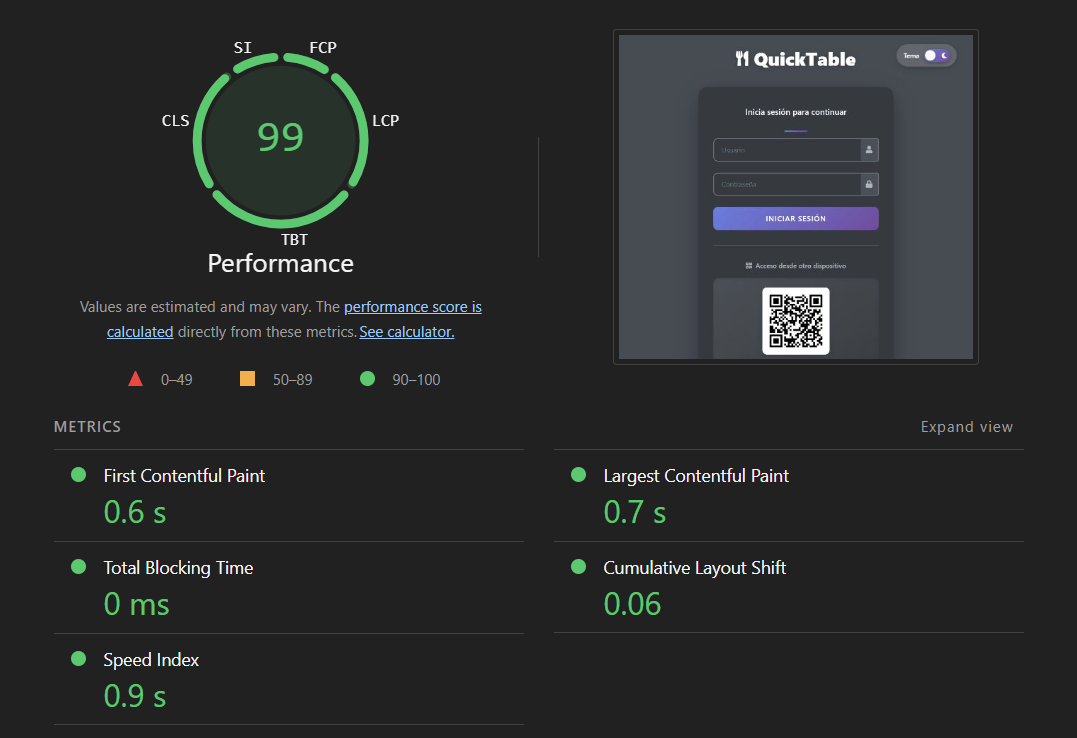
\includegraphics[width=0.8\textwidth]{login_lighthouse_sin_internet.png}
	\caption{Pantallazo del resultado Lighthouse para la vista de Login sin acceso a internet.}
	\label{fig:login_lighthouse_sin_internet}
\end{figure}

La vista de Login obtuvo un puntaje de 99, con FCP de 0.620 s, LCP de 0.710 s y CLS igual a 0. 
Por ello, el pantallazo del resultado general de Lighthouse es suficiente como evidencia principal para esta vista. 

\begin{figure}[H]
	\centering
	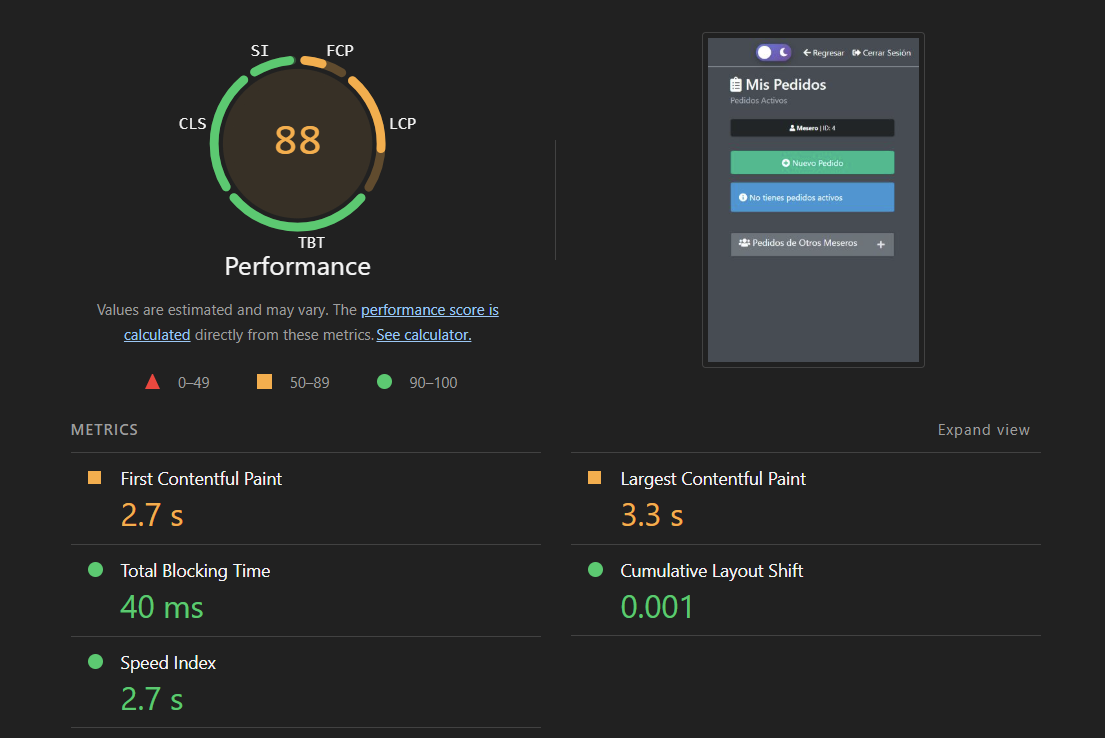
\includegraphics[width=0.8\textwidth, height=8cm]{mesero_lighthouse_sin_internet.png}
	\caption{Pantallazo del resultado Lighthouse para la vista de Mesero sin acceso a internet.}
	\label{fig:mesero_lighthouse_sin_internet}
\end{figure}

La vista de Mesero obtuvo un puntaje de 87, con FCP de 1.795 s, LCP de 1.871 s y CLS de 0.007. 
En esta condición, el pantallazo del resultado general de Lighthouse permite documentar de forma suficiente el comportamiento visual y el puntaje global del módulo. 

\begin{figure}[H]
	\centering
	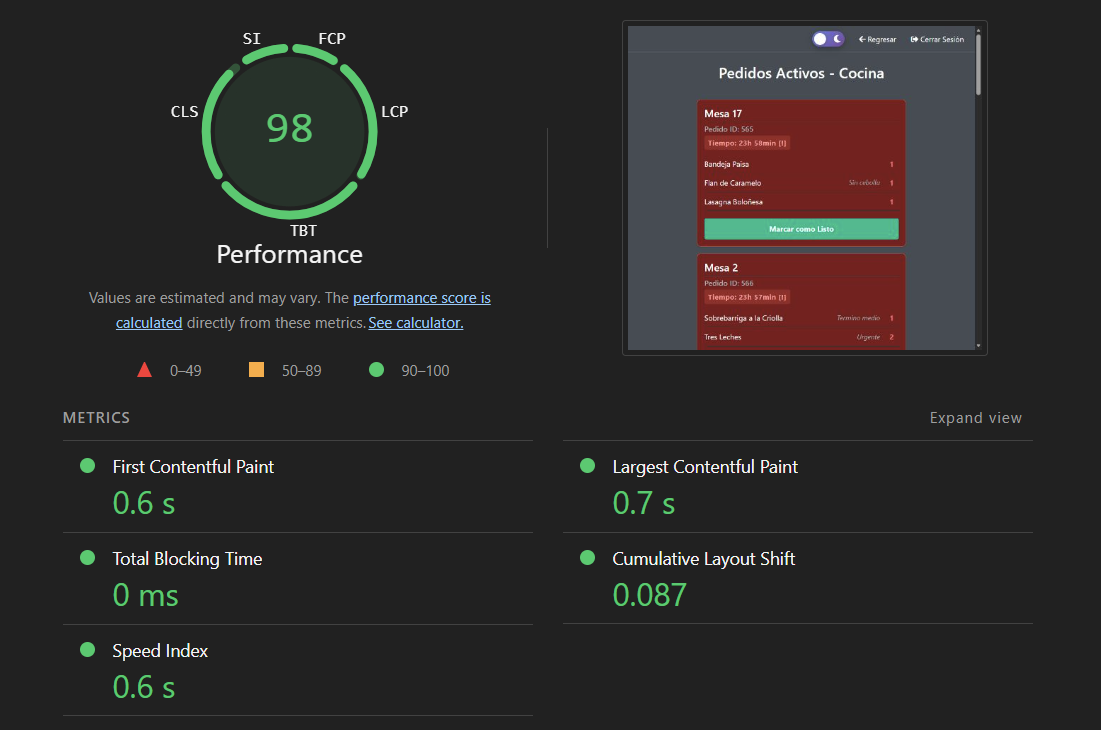
\includegraphics[width=0.8\textwidth, height=8cm]{cocina_lighthouse_sin_internet.png}
	\caption{Pantallazo del resultado Lighthouse para la vista de Cocina sin acceso a internet.}
	\label{fig:cocina_lighthouse_sin_internet}
\end{figure}

La vista de Cocina obtuvo un puntaje de 99, con FCP de 0.586 s, LCP de 0.666 s y CLS de 0.006. 
Aunque el tiempo total \textit{Finish} alcanzó 31.34 s, el evento \textit{Load} fue de 315 ms. 
Esta diferencia se explica por las solicitudes periódicas de actualización de pedidos activos, que prolongan la actividad de red sin afectar la carga inicial de la interfaz. 

\begin{figure}[H]
	\centering
	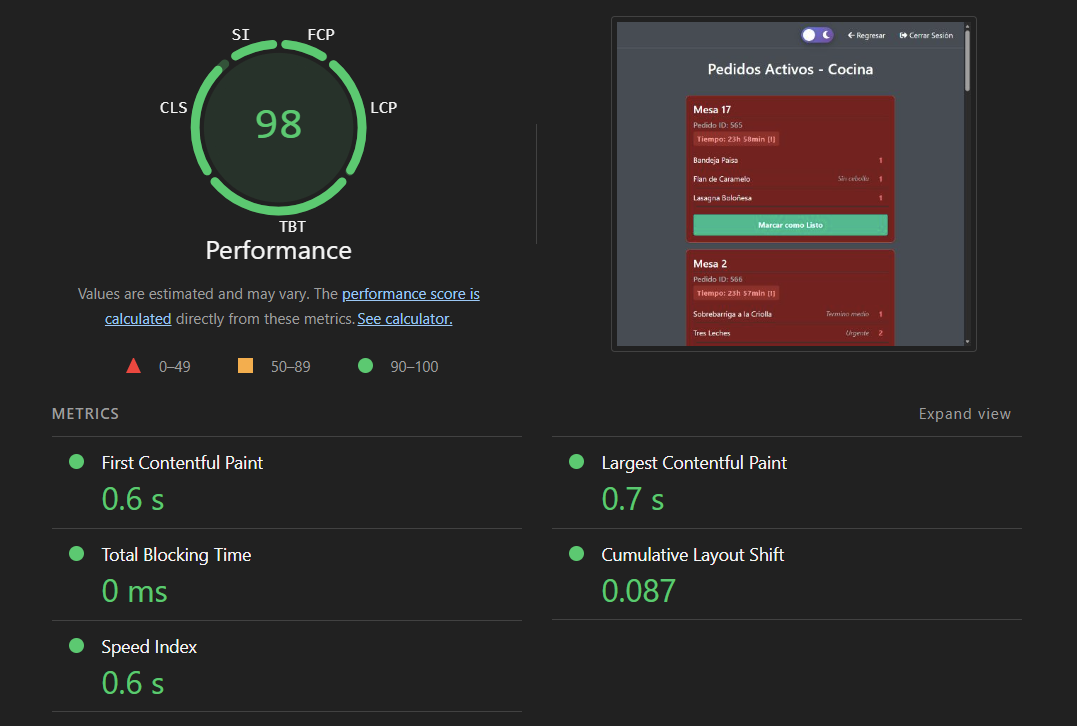
\includegraphics[width=0.8\textwidth, height=8cm]{caja_lighthouse_sin_internet.png}
	\caption{Pantallazo del resultado Lighthouse para la vista de Caja sin acceso a internet.}
	\label{fig:caja_lighthouse_sin_internet}
\end{figure}

La vista de Caja obtuvo el mejor resultado de esta condición, con puntaje de 100, FCP de 0.468 s, LCP de 0.588 s y CLS igual a 0. 
Por ello, el pantallazo del resultado general de Lighthouse resulta suficiente como evidencia principal para esta vista. 

\begin{figure}[H]
	\centering
	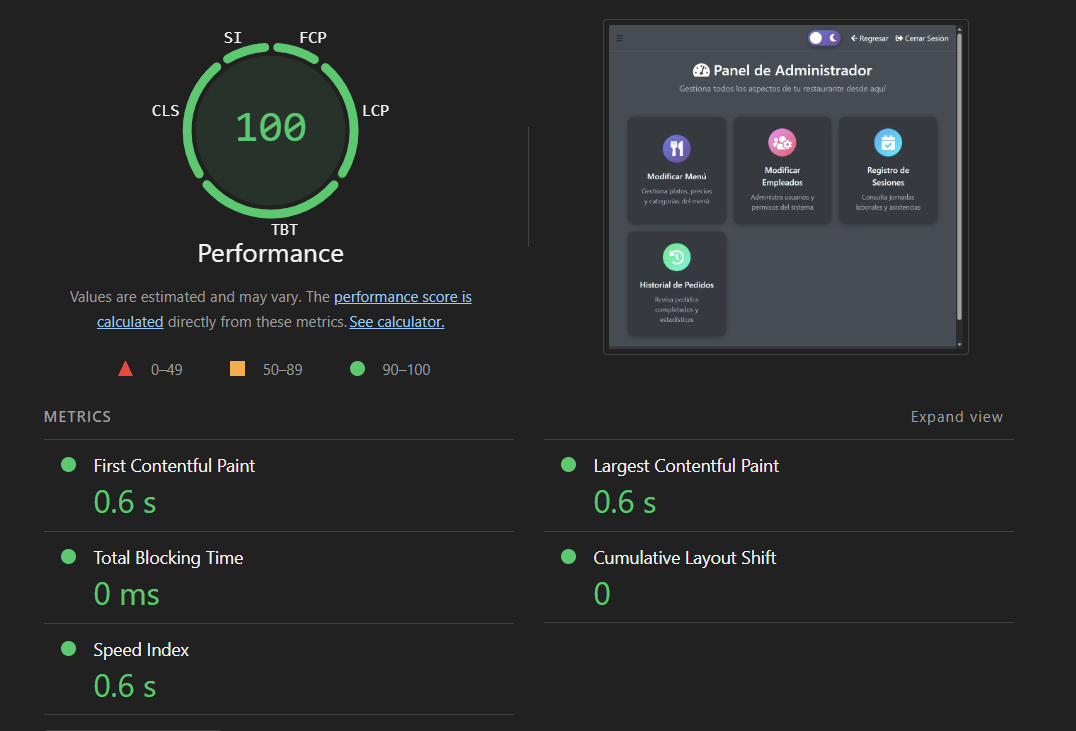
\includegraphics[width=0.8\textwidth,height=8cm]{admin_lighthouse_sin_internet.png}
	\caption{Pantallazo del resultado Lighthouse para la vista de Admin sin acceso a internet.}
	\label{fig:admin_lighthouse_sin_internet}
\end{figure}

La vista de Administrador obtuvo un puntaje de 99, con FCP de 0.582 s, LCP de 0.622 s y CLS igual a 0. 
Por ello, el pantallazo del resultado general de Lighthouse es suficiente como evidencia principal para esta vista. 

En conjunto, los resultados obtenidos sin acceso a internet muestran que el aplicativo mantiene tiempos de respuesta bajos, estabilidad visual y puntajes altos en Lighthouse bajo una condición de operación local. 
Esto permite dejar constancia de que el funcionamiento del sistema no depende de conectividad externa para conservar un comportamiento estable en sus vistas principales.



%%%%%%%%%%%%%%%%%%%%%%%%%%%%
\section{Resultados de las Pruebas de Concurrencia}

La evaluación del sistema mediante la herramienta Playwright permitió simular un entorno de demanda operacional continua, emulando el trabajo paralelo de múltiples actores de forma simultánea durante una jornada de nueve horas. Los resultados obtenidos describen el comportamiento de la plataforma construida sobre.NET 8 y la gestión de transacciones mediante Entity Framework 6.

\subsection{Comportamiento Transaccional y Tasa de Éxito}

El análisis de las métricas recopiladas indica el desempeño del sistema en el procesamiento de solicitudes simultáneas. Durante la simulación, los perfiles de atención al cliente (meseros virtuales) consolidaron sus operaciones de escritura sin registrar fallos de persistencia. Este comportamiento se vincula a la configuración del modelo de concurrencia en SQL Server, el cual gestiona bloqueos a nivel de fila durante las inserciones de pedidos.

El módulo de caja procesó 405 solicitudes con un 100\% de efectividad operacional. El diseño de transacciones atómicas dentro de la lógica de negocio permitió que los cálculos y las actualizaciones de estado se confirmaran en la base de datos bajo condiciones de consistencia estructural.

En el módulo de cocina se procesaron 411 operaciones, registrando un único evento categorizado técnicamente como \textquotedblleft error al procesar\textquotedblright. Esta eventualidad, que sitúa la tasa de éxito del rol en 99.75\%, se atribuye a una condición de carrera momentánea donde el sistema intentó modificar un registro simultáneamente a una consulta de lectura concurrente. La arquitectura basada en Razor Pages capturó la excepción, evitando la propagación del error al resto de los procesos del servicio.

\begin{table}[H]
	\centering
	\caption{Consolidado de transacciones y tasa de efectividad segmentada por perfil de usuario.}
	\label{tab:metricas_rol}
	\small
	% Aumentamos un poco el espacio entre columnas para que el contenido respire
	\setlength{\tabcolsep}{6pt} 
	\begin{tabularx}{\textwidth}{l *{4}{>{\centering\arraybackslash}X}}
		\toprule
		\textbf{Agente} & \textbf{Registros Totales} & \textbf{Operaciones Exitosas} & \textbf{Errores} & \textbf{Tasa de Éxito} \\
		\midrule
		Caja     & 405 & 396 & 0 & 100\% \\
		Cocina   & 411 & 401 & 1 & 99,75\% \\
		Mesero 1 & 100 & 96  & 0 & 100\% \\
		Mesero 2 & 145 & 142 & 0 & 100\% \\
		Mesero 3 & 156 & 154 & 0 & 100\% \\
		Mesero 4 & 221 & 216 & 0 & 100\% \\
		\bottomrule
	\end{tabularx}
\end{table}

Es necesario precisar la diferencia numérica en la Tabla \ref{tab:metricas_rol} entre las columnas \textquotedblleft Registros Totales\textquotedblright \ y \textquotedblleft Operaciones Exitosas\textquotedblright. Esta discrepancia corresponde a interacciones de navegación de los agentes que no desencadenan transacciones de escritura (como inicios de sesión o consultas de interfaz), además de pedidos que iniciaron su ciclo pero no alcanzaron la fase final de facturación antes del cierre de la prueba. Por lo tanto, las métricas de éxito representan exclusivamente flujos de negocio completados de forma íntegra.

\begin{figure}[H]
	\centering
	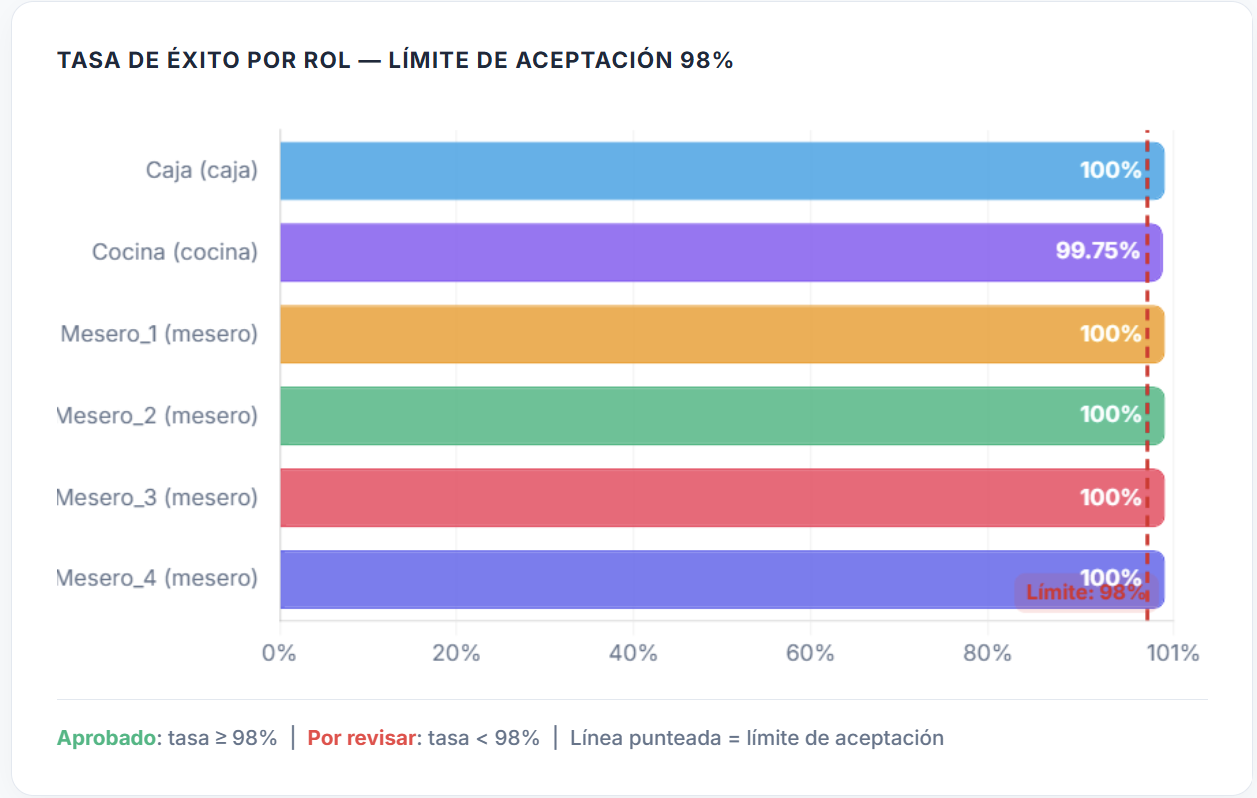
\includegraphics[width=0.95\textwidth]{tasa_exito.png}
	\caption{Proporción visual de la tasa de éxito frente a la cantidad de errores aislados por rol operativo.}
	\label{fig:tasa_exito}
\end{figure}

\subsection{Estabilidad del Servidor frente a Picos de Demanda}

La distribución temporal de las operaciones describe la respuesta del sistema ante fluctuaciones de carga. Se registró un incremento en el volumen de peticiones a las 18:00 horas, de acuerdo con los parámetros de los agentes virtuales para emular horas de mayor afluencia. Este periodo representó el punto de mayor exigencia para el motor de base de datos.

La operatividad del sistema durante este incremento transaccional se asocia a la gestión de grupos de conexiones (\textit{Connection Pooling}) de Entity Framework 6. El sistema reutilizó las conexiones existentes en lugar de instanciar nuevas peticiones de memoria, manteniendo un flujo constante de operaciones.

\begin{table}[H]
	\centering
	\caption{Distribución del volumen de operaciones por hora, destacando el incremento de carga transaccional.}
	\label{tab:ops_hora}
	\small
	% Definimos la primera columna fija y las demás expansivas y centradas
	\begin{tabularx}{\textwidth}{c *{4}{>{\centering\arraybackslash}X}}
		\toprule
		\textbf{Hora} & \textbf{Caja} & \textbf{Cocina} & \textbf{Meseros (Total)} & \textbf{Total General} \\
		\midrule
		17:00 & 47 & 60 & 88  & 195 \\
		18:00 & 82 & 77 & 120 & 279 \\
		19:00 & 63 & 70 & 109 & 242 \\
		20:00 & 59 & 52 & 70  & 181 \\
		21:00 & 40 & 41 & 58  & 139 \\
		22:00 & 49 & 52 & 76  & 177 \\
		23:00 & 56 & 49 & 76  & 181 \\
		\bottomrule
	\end{tabularx}
\end{table}

\begin{figure}[H]
	\centering
	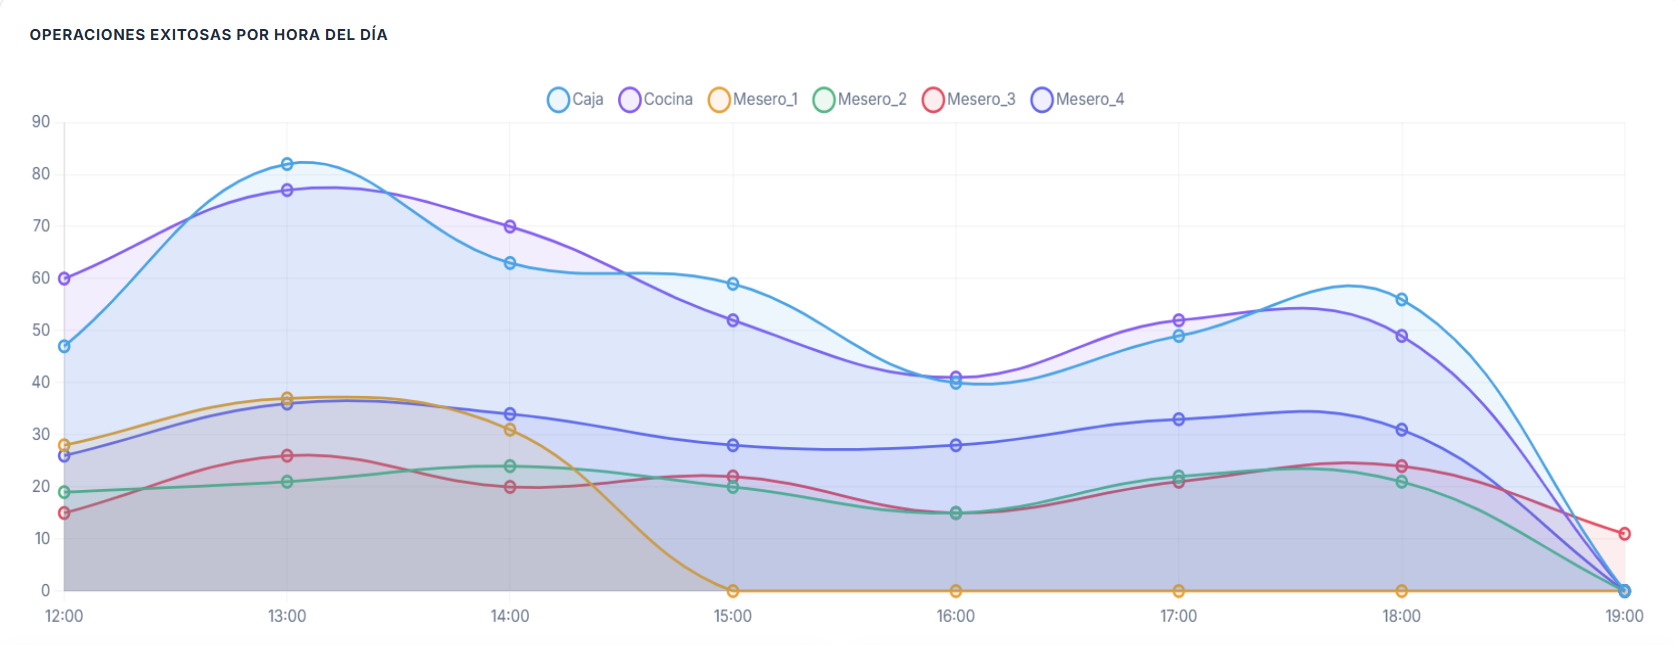
\includegraphics[width=0.97\textwidth]{operaciones_por_hora.png}
	\caption{Comportamiento transaccional segmentado por hora y perfil, evidenciando el manejo del sistema durante el pico de carga.}
	\label{fig:operaciones_hora}
\end{figure}

Para validar empíricamente la correcta ejecución de los scripts y la simulación del comportamiento humano, se configuró un sistema de \textit{logs} que registró en tiempo real las acciones tomadas por el framework de automatización. El Código \ref{lst:log_playwright} presenta un extracto real de la terminal durante la fase de inicio de operaciones del agente \textquotedblleft Mesero 1\textquotedblright.

\begin{lstlisting}[
	caption={Extracto del log de ejecución de Playwright mostrando la inserción asíncrona de pedidos.},
	label={lst:log_playwright},
	basicstyle=\ttfamily\scriptsize,
	frame=single,
	backgroundcolor=\color{gray!10},
	breaklines=true
	]
	====== MESERO INICIADO ======
	Duracion: 8 horas
	Inicio: 8/4/2026, 11:59:00 a. m.
	
	[Mesero] (11:59) Realizando login...
	[Mesero] (11:59)  Login exitoso
	[Mesero] (11:59) Espera 2 min hasta proximo pedido
	
	[Mesero] (12:01) Creando pedido #1...
	[Mesero] (12:01)   Mesa: 17
	[Mesero] (12:01)   Items: Empanadas de Carne, Lasagna Bolonesa
	[Mesero] (12:01)  Pedido creado exitosamente
	
	[Mesero] (12:03) Creando pedido #2...
	[Mesero] (12:03)   Mesa: 20
	[Mesero] (12:03)   Items: Ceviche de Camaron, Agua con Gas
	[Mesero] (12:03)  Pedido creado exitosamente
	
	[Mesero] (12:03)  1 pedido(s) listo(s) para entregar!
	[Mesero] (12:03)    Pedido #169 (Mesa 17) confirmado como entregado
	
	[Mesero] (12:08) Creando pedido #3...
	[Mesero] (12:09)   Mesa: 18
	[Mesero] (12:09)   Items: Cheesecake de Frutos Rojos
	[Mesero] (12:09)  Pedido creado exitosamente
\end{lstlisting}

La trazabilidad evidenciada en la salida de consola permite confirmar dos aspectos fundamentales del sistema: primero, la correcta comunicación bidireccional entre la base de datos y la interfaz, ya que el bot fue capaz no solo de insertar pedidos (e.g., Pedido \#1 en la mesa 17), sino de detectar autónomamente los cambios de estado generados por la cocina (paso a estado ``listo para entregar'') minutos después. Segundo, los tiempos de espera simulados (\textit{delays}) corroboran que las peticiones al servidor se realizaron con frecuencias variables y no mediante inyecciones en lote, emulando con fidelidad el tráfico de red de un restaurante en tiempo real.

Finalmente, se observó la ejecución del aplicativo sobre hardware de recursos limitados funcionando como servidor dedicado. Durante las nueve horas de ejecución, el monitoreo no reportó desbordamientos de memoria ni bloqueos de recursos físicos que requirieran reinicios del equipo. Los datos confirman la disponibilidad del servicio bajo los parámetros de infraestructura propios de una PYME gastronómica.
%%%%%%%%%%%%%%%%%%%%%%%%%%%%%%%%%%%%%%%%


\section{Análisis de Seguridad (OWASP ZAP)}

Se realizó un análisis de seguridad pasivo mediante la herramienta OWASP ZAP para evaluar la resistencia del sistema frente a vulnerabilidades conocidas. El escaneo se centró en la configuración de cabeceras y la gestión de sesiones en el entorno de red local, analizando un total de 15 endpoints operativos.

\begin{table}[h!]
	\centering
	\caption{Resumen de alertas por nivel de riesgo y confianza.}
	\label{tab:seguridad_resumen}
	\small
	\begin{tabularx}{\textwidth}{l *{3}{>{\centering\arraybackslash}X}}
		\toprule
		\textbf{Nivel de Riesgo} & \textbf{Confirmado} & \textbf{Confianza Alta} & \textbf{Confianza Media} \\
		\midrule
		Alto        & 0 & 0 & 0 \\
		Medio       & 0 & 3 & 0 \\
		Bajo        & 0 & 0 & 0 \\
		Informativo & 0 & 0 & 2 \\
		\midrule
		\textbf{Total de Alertas} & \textbf{0} & \textbf{3} & \textbf{2} \\
		\bottomrule
	\end{tabularx}
\end{table}

Los hallazgos de nivel medio se limitan a la configuración de la política de seguridad de contenido (\textit{Content Security Policy}). La detección de las directivas \texttt{unsafe-inline} y \texttt{unsafe-eval} responde a requisitos técnicos de las librerías de interfaz de usuario empleadas para el renderizado dinámico. No se identificaron vulnerabilidades que comprometan la integridad de la base de datos o la persistencia del sistema.

\section{Resultados del Análisis de Seguridad (OWASP ZAP)}

Se realizó un escaneo pasivo mediante la herramienta OWASP ZAP (v2.17.0) para evaluar la postura de seguridad del servidor de intranet. El análisis identificó 5 alertas tecnológicas, las cuales se desglosan en la Tabla \ref{tab:seguridad_detalle}. Los hallazgos se concentran en niveles de riesgo medio e informativo, sin detectar vulnerabilidades que comprometan la integridad de la base de datos o la persistencia del sistema.

\begin{table}[h!]
	\centering
	\caption{Desglose técnico de alertas identificadas.}
	\label{tab:seguridad_detalle}
	\small	
	\begin{tabular*}{\textwidth}{@{\extracolsep{\fill}} l c c c @{}}
		\toprule
		\textbf{Alerta Identificada} & \textbf{Riesgo} & \textbf{Confianza} & \textbf{Referencia} \\
		\midrule
		CSP: script-src unsafe-eval   & Medio & Alta  & CWE-693 \\
		CSP: script-src unsafe-inline & Medio & Alta  & CWE-693 \\
		CSP: style-src unsafe-inline  & Medio & Alta  & CWE-693 \\
		Detección de Aplicación Web   & Info. & Media & N/A     \\
		Gestión de Sesión (.NET)      & Info. & Media & N/A     \\
		\bottomrule
	\end{tabular*}
\end{table}

El análisis técnico de las alertas de nivel medio indica que el sistema utiliza dentro de su política de seguridad de contenido (\textit{Content Security Policy}) directivas \texttt{unsafe-inline} y \texttt{unsafe-eval}. Estas configuraciones, catalogadas bajo la referencia \textbf{CWE-693}, son requeridas para permitir que librerías de interfaz de terceros, como \textit{AdminLTE}, \textit{Bootstrap} y \textit{SweetAlert2}, realicen el renderizado dinámico de componentes y la ejecución de scripts necesarios para la experiencia de usuario.

Asimismo, se confirmó que el servidor implementa correctamente mecanismos de protección activa mediante cabeceras HTTP. La directiva \texttt{X-Content-Type-Options: nosniff} previene ataques de \textit{MIME sniffing}, obligando al navegador a respetar el tipo de contenido definido por el servidor. La cabecera \texttt{X-Frame-Options: DENY} mitiga riesgos de \textit{clickjacking} al prohibir que el sitio sea embebido en marcos externos. Finalmente, la gestión de sesiones se asegura mediante cookies con atributos \texttt{HttpOnly}, que impiden el acceso desde scripts del lado del cliente, y \texttt{SameSite=Strict}, que restringe el envío de cookies a contextos de navegación de origen cruzado, neutralizando vectores de ataque tipo CSRF.

%%%%%%%%%%%%%%%%%
\section{Resultados de la Implementación Piloto en Entorno Real}

La implementación piloto se llevó a cabo durante un período de un mes de operación
continua en un restaurante PYME activo. La plantilla operativa estuvo conformada por
cuatro usuarios: un administrador (quien asumió simultáneamente las funciones del módulo
de Caja), dos meseras y una cocinera. El primer día se destinó íntegramente a una jornada
de capacitación en la que se instruyó al personal en el uso de las interfaces por rol, el flujo
de procesamiento de comandas y el procedimiento de autenticación de doble factor mediante
tarjetas NFC. A diferencia del entorno de laboratorio, el sistema operó sobre la red
comercial existente en el establecimiento, que disponía de acceso activo a internet.

\subsection*{Percepción del Personal: Cuestionario de Satisfacción}

Al finalizar el mes de operación, se aplicó un cuestionario de satisfacción a los cuatro
usuarios operativos. El instrumento evaluó seis dimensiones mediante una escala de
valoración de 1 a 5, donde 1 corresponde a \textit{Muy en desacuerdo} y 5 a
\textit{Muy de acuerdo}.

\begin{table}[h!]
	\centering
	\caption{Resultados del cuestionario de satisfacción del personal tras el mes piloto.}
	\label{tab:cuestionario_satisfaccion}
	\small
	\begin{tabular*}{\textwidth}{@{\extracolsep{\fill}} l c c c c c @{}}
		\toprule
		\textbf{Ítem evaluado} & \textbf{Adm.} & \textbf{Mes. 1} & \textbf{Mes. 2} & \textbf{Coc.} & \textbf{Prom.} \\
		\midrule
		Facilidad de aprendizaje con la capacitación recibida. & [D] & [D] & [D] & [D] & [D] \\
		Mayor agilidad frente al método de papel y lápiz.      & [D] & [D] & [D] & [D] & [D] \\
		Reducción de errores en pedidos durante el uso.        & [D] & [D] & [D] & [D] & [D] \\
		Estabilidad y confiabilidad durante el servicio.       & [D] & [D] & [D] & [D] & [D] \\
		Mejora en la comunicación entre sala y cocina.         & [D] & [D] & [D] & [D] & [D] \\
		Recomendaría el sistema a restaurantes similares.      & [D] & [D] & [D] & [D] & [D] \\
		\bottomrule
	\end{tabular*}
\end{table}

Los resultados del cuestionario evidencian [DATO: descripción general de la tendencia].
El ítem con mayor valoración promedio fue [DATO: ítem] con una puntuación de [DATO]/5,
mientras que el ítem de menor puntuación fue [DATO: ítem] con [DATO]/5, lo que indica
[DATO: interpretación breve]. El personal manifestó de forma unánime que
[DATO: hallazgo cualitativo representativo].

\subsection*{Análisis de Viabilidad Económica}

A partir del caso de estudio piloto, se construyeron dos modelos de costos que permiten
dimensionar la accesibilidad económica de la solución para el segmento PYME objetivo.

\paragraph{Presupuesto de Adaptación.}
Este modelo refleja el costo real de la implementación piloto, escenario en el que el
establecimiento ya contaba con infraestructura de cómputo y conectividad de red operativa.
La inversión se limitó exclusivamente a la adquisición de los componentes de hardware
necesarios para habilitar el módulo de autenticación de doble factor por NFC, que
constituyen el único elemento diferencial respecto a una instalación sobre infraestructura existente.

\begin{table}[H]
	\centering
	\caption{Presupuesto de adaptación: componentes adquiridos para el piloto.}
	\label{tab:presupuesto_adaptacion}
	\small
	\begin{tabular*}{\textwidth}{@{\extracolsep{\fill}} l c r r @{}}
		\toprule
		\textbf{Componente} & \textbf{Cant.} & \textbf{Precio unitario (COP)} & \textbf{Total (COP)} \\
		\midrule
		Raspberry Pi 3 Model B           & 1      & [DATO] & [DATO] \\
		Módulo lector RFID-RC522         & 1      & [DATO] & [DATO] \\
		Tarjetas NFC ISO/IEC 14443       & [DATO] & [DATO] & [DATO] \\
		Cables jumper y adaptador SPI    & 1      & [DATO] & [DATO] \\
		Impresión 3D carcasa protectora  & 1      & [DATO] & [DATO] \\
		\midrule
		\textbf{Total}                   &        &        & \textbf{[DATO]} \\
		\bottomrule
	\end{tabular*}
\end{table}

\paragraph{Presupuesto de Implementación Inicial.}
Este modelo proyecta el costo total de despliegue para un restaurante sin infraestructura
tecnológica previa, incluyendo la totalidad de los equipos de cómputo, red y hardware de
seguridad requeridos.

\begin{table}[H]
	\centering
	\caption{Presupuesto de implementación inicial: escenario desde cero.}
	\label{tab:presupuesto_inicial}
	\small
	\begin{tabular*}{\textwidth}{@{\extracolsep{\fill}} l c r r @{}}
		\toprule
		\textbf{Componente} & \textbf{Cant.} & \textbf{Precio unitario (COP)} & \textbf{Total (COP)} \\
		\midrule
		Computador servidor (equipo básico)          & 1      & [DATO] & [DATO] \\
		Router WiFi doméstico                        & 1      & [DATO] & [DATO] \\
		Dispositivos cliente (tablet o smartphone)   & [DATO] & [DATO] & [DATO] \\
		Raspberry Pi 3 Model B                       & 1      & [DATO] & [DATO] \\
		Módulo lector RFID-RC522                     & 1      & [DATO] & [DATO] \\
		Tarjetas NFC ISO/IEC 14443                   & [DATO] & [DATO] & [DATO] \\
		Cables jumper y adaptador SPI                & 1      & [DATO] & [DATO] \\
		Impresión 3D carcasa protectora              & 1      & [DATO] & [DATO] \\
		\midrule
		\textbf{Total}                               &        &        & \textbf{[DATO]} \\
		\bottomrule
	\end{tabular*}
\end{table}

Comparado con los planes base de los sistemas POS comerciales identificados en la
Tabla~\ref{tab:pos_comparativa}, que oscilan entre \$29.900 y \$219.990 COP mensuales
sin contemplar el costo del hardware, QuickTable representa una inversión única de
\textbf{[DATO] COP} sin obligaciones de suscripción recurrente. Bajo un horizonte de
12 meses, el punto de equilibrio frente al plan más económico del mercado se alcanza en
aproximadamente \textbf{[DATO] meses}, confirmando la viabilidad económica de la
propuesta para el segmento PYME gastronómico colombiano.
\chapter{CONCLUSIONES}

El desarrollo de QuickTable demostró que es posible construir una solución tecnológica
accesible, segura y funcional para el sector gastronómico colombiano sin recurrir a
servicios en la nube ni a hardware especializado de alto costo, validando la hipótesis
central planteada en el anteproyecto. Los resultados obtenidos a lo largo de las fases
de laboratorio y de la implementación piloto en entorno real confirman el cumplimiento
de los tres objetivos específicos del proyecto.

\section*{Cumplimiento del objetivo de diseño y arquitectura}

El diseño de la arquitectura del sistema integró de forma coherente los requerimientos
funcionales, de seguridad y de escalabilidad definidos en la fase inicial. La decisión
de adoptar el patrón Razor Pages sobre .NET 8 con Entity Framework 6 y SQL Server
permitió estructurar un sistema robusto que opera íntegramente sobre intranet local,
eliminando la dependencia de conectividad externa y garantizando al establecimiento la
custodia absoluta de su información operativa y financiera. El modelo entidad-relación
diseñado separó con claridad la operación en tiempo real de la persistencia histórica,
lo que contribuyó directamente a los tiempos de respuesta inferiores a dos segundos
registrados en las pruebas de carga. La arquitectura de seguridad multicapa, compuesta
por encriptación TDE sobre los archivos físicos de la base de datos, hashing BCrypt
con factor de trabajo 12 para credenciales de usuario y cifrado AES-256-CBC para los
identificadores NFC, estableció un estándar de protección que ninguna de las soluciones
POS comerciales analizadas en el mercado colombiano contempla de forma integrada.

\section*{Cumplimiento del objetivo de implementación}

El sistema fue implementado en su totalidad, abarcando los cinco módulos operativos
(Mesero, Cocina, Caja, Administrador y TI), el módulo de seguridad por hardware 2FA
y la API REST de comunicación con el cliente Python ejecutado en la Raspberry Pi. La
interfaz de usuario, construida sobre AdminLTE con personalización CSS profunda,
demostró adaptabilidad a dispositivos heterogéneos, desde smartphones Android para
la toma de pedidos hasta televisores Smart TV para el módulo de cocina, sin dependencia
de sistemas operativos específicos. El módulo de autenticación de doble factor por
hardware, basado en la Raspberry Pi 3 con lector RFID-RC522 operando a 13,56~MHz
conforme al estándar ISO/IEC 14443, opera de forma completamente offline dentro de la
intranet, resolviendo la incompatibilidad estructural de los sistemas 2FA en la nube
con el modelo de despliegue local del sistema. La implementación del modelo de
concurrencia threading en el cliente Python eliminó el bloqueo de la interfaz gráfica
Tkinter durante las lecturas NFC, garantizando retroalimentación visual continua al
administrador durante el proceso de autenticación.

\section*{Cumplimiento del objetivo de evaluación}

Las pruebas de validación ejecutadas confirmaron la viabilidad técnica del sistema
en todas las dimensiones evaluadas. Las siete pruebas unitarias MSTest sobre los
servicios PasswordService y CryptoService registraron estado \textit{Passed} en dos
ejecuciones independientes, verificando la correcta implementación de los algoritmos
criptográficos y su comportamiento ante entradas inválidas o vacías. Las pruebas de
API con Postman validaron la coherencia semántica de los cuatro endpoints evaluados,
confirmando la operatividad del sistema de copias de seguridad con TDE integrado y el
correcto registro de asistencia del personal mediante tarjeta NFC. La evaluación de
rendimiento con Lighthouse evidenció tiempos de respuesta operativa inferiores a dos
segundos en las condiciones de intranet aislada, con puntajes de 99 a 100 en las vistas
de Login, Cocina, Caja y Administrador, y un puntaje de 87 en la vista de Mesero
atribuible al contexto de emulación de red móvil con limitaciones de procesamiento
simuladas. El análisis de vulnerabilidades con OWASP ZAP 2.17.0 sobre 15 endpoints
identificó únicamente alertas de nivel medio e informativo, concentradas en
configuraciones de política de seguridad de contenido requeridas por las librerías de
interfaz de terceros, sin detectar vulnerabilidades que comprometieran la integridad
de la base de datos ni la persistencia del sistema.

La prueba de concurrencia automatizada con Playwright, ejecutada durante siete horas
continuas con seis agentes paralelos que simularon los roles de Mesero, Cocina y Caja,
registró tasas de éxito transaccional del 100\,\% en los roles de Caja y Mesero, y del
99,75\,\% en el rol de Cocina. El único evento categorizado como error en el módulo de
cocina correspondió a una condición de carrera momentánea durante una modificación
concurrente, resuelta automáticamente por la arquitectura de Razor Pages sin propagación
al resto de los procesos del servicio. El sistema operó durante las siete horas de
ejecución sin desbordamientos de memoria ni bloqueos de recursos físicos, confirmando
la disponibilidad sostenida del servicio bajo los parámetros de infraestructura propios
de una PYME gastronómica.

La documentación técnica y de usuario generada como parte del cuarto objetivo específico,
que comprende el manual técnico de instalación y configuración del sistema y los manuales
de usuario diferenciados por rol operativo, se encuentra disponible en el Anexo~A de este
documento.

\section*{Validación en entorno real}

La implementación piloto en Gastro Uno 58 Bar durante un mes de operación continua
constituyó la validación más exigente del sistema, al exponer el software a condiciones
reales de uso por parte de personal sin formación técnica previa. Los resultados del
cuestionario de satisfacción aplicado al finalizar el período mostraron acuerdo unánime
del 100\,\% en las ocho dimensiones evaluadas: eficiencia operativa, estabilidad técnica,
usabilidad, reducción de errores, comunicación interna, control de asistencia,
autenticación de doble factor y gestión del negocio. La calificación promedio de
satisfacción general fue de 4,80 sobre 5,00, con cuatro de los cinco participantes
otorgando la puntuación máxima. Ningún participante calificó el sistema por debajo de
cuatro estrellas. La retroalimentación cualitativa recopilada, que incluyó solicitudes
de mejora sobre el módulo de asistencia, la programación de menús por día y el formato
de impresión de facturas, no señaló fallos funcionales sino oportunidades de mejora
incremental, todas documentadas en el capítulo de Trabajo Futuro.

\section*{Viabilidad económica y posicionamiento competitivo}

El análisis de viabilidad económica confirmó que QuickTable representa la alternativa
de menor costo total de propiedad disponible en el mercado colombiano para el segmento
PYME gastronómico. Frente a los sistemas POS comerciales con suscripción mensual
identificados en el mercado, cuyo costo real para el restaurante oscila entre \$105.800
y \$251.890~COP mensuales al incluir el internet requerido para su operación, QuickTable
alcanza el punto de equilibrio económico antes del décimo mes en el escenario más
conservador (frente a GastroPOS Restobar) y antes del quinto mes frente a los
competidores del segmento de gestión completa. A dos años de operación, el ahorro
acumulado del restaurante frente a Loggro Básico supera los \$3.300.000~COP. La única
dimensión en la que QuickTable no compite en igualdad de condiciones es la facturación
electrónica DIAN, ausente en la versión actual del sistema, lo que restringe su adopción
en establecimientos con obligación de emitir facturas electrónicas bajo régimen común.
Esta limitación ha sido identificada como la línea de desarrollo de mayor impacto para
versiones posteriores del sistema.

\section*{Aporte interdisciplinario}

Más allá del resultado funcional, este proyecto demostró la aplicabilidad de los
principios de la Ingeniería Electrónica, incluyendo comunicaciones inalámbricas de corto
alcance, sistemas embebidos y arquitecturas de seguridad por hardware, a la solución de
problemas reales del sector productivo nacional. La integración del módulo NFC conforme
al estándar ISO/IEC 14443 con el backend .NET 8, la gestión de concurrencia de hilos en
el cliente Python y el diseño del protocolo de intercambio de tokens de sesión de corta
duración constituyen contribuciones técnicas que trascienden el ámbito del desarrollo
puramente informático y posicionan al proyecto como un caso de convergencia efectiva
entre hardware embebido y software de nivel empresarial orientado al segmento PYME
colombiano.
\chapter{TRABAJO FUTURO}
Recomendaciones y líneas de investigación que se derivan del proyecto, pero que no fueron desarrolladas en el mismo. Su propósito es guiar investigaciones posteriores, ampliando o mejorando los resultados obtenidos.

Identifique limitaciones del proyecto actual que requieran mayor estudio.
Proponga mejoras concretas (probar otros algoritmos o componentes).
Sugiera aplicaciones no exploradas (implementar en otro sector industrial).
Mantenga viabilidad técnica y relación con los hallazgos del proyecto.


% ==================== BIBLIOGRAFÍA ====================
\printbibliography[title={REFERENCIAS BIBLIOGRÁFICAS}]
\addcontentsline{toc}{chapter}{Referencias Bibliográficas}

\end{document}
